\documentclass[a4paper]{book}
\usepackage{makeidx}
\usepackage{graphicx}
\usepackage{multicol}
\usepackage{float}
\usepackage{listings}
\usepackage{color}
\usepackage{ifthen}
\usepackage[table]{xcolor}
\usepackage{textcomp}
\usepackage{alltt}
\usepackage{ifpdf}
\ifpdf
\usepackage[pdftex,
            pagebackref=true,
            colorlinks=true,
            linkcolor=blue,
            unicode
           ]{hyperref}
\else
\usepackage[ps2pdf,
            pagebackref=true,
            colorlinks=true,
            linkcolor=blue,
            unicode
           ]{hyperref}
\usepackage{pspicture}
\fi
\usepackage[utf8]{inputenc}
\usepackage{mathptmx}
\usepackage[scaled=.90]{helvet}
\usepackage{courier}
\usepackage{sectsty}
\usepackage[titles]{tocloft}
\usepackage{doxygen}
\lstset{language=C++,inputencoding=utf8,basicstyle=\footnotesize,breaklines=true,breakatwhitespace=true,tabsize=8,numbers=left }
\makeindex
\setcounter{tocdepth}{3}
\renewcommand{\footrulewidth}{0.4pt}
\renewcommand{\familydefault}{\sfdefault}
\begin{document}
\hypersetup{pageanchor=false}
\begin{titlepage}
\vspace*{7cm}
\begin{center}
{\Large AMORE++ \\[1ex]\large pre-\/alpha (active development aiming to release a beta version this summer (2011) ) }\\
\vspace*{1cm}
{\large Generated by Doxygen 1.7.4}\\
\vspace*{0.5cm}
{\small Sat Jul 16 2011 10:53:54}\\
\end{center}
\end{titlepage}
\clearemptydoublepage
\pagenumbering{roman}
\tableofcontents
\clearemptydoublepage
\pagenumbering{arabic}
\hypersetup{pageanchor=true}
\chapter{The AMORE++ package}
\label{index}\hypertarget{index}{}\hypertarget{main_intro_sec}{}\section{Introduction}\label{main_intro_sec}
Here you will find the documentation of the C++ component of the AMORE++ R package.

The AMORE++ package is a new version of the publicly available AMORE package for neural network training and simulation under R\hypertarget{main_motiv_sec}{}\section{Motivation}\label{main_motiv_sec}
Since the release of the previous version of the AMORE many things have changed in the R programming world.

The advent of the Reference Classes and of packages like Rcpp, inline and RUnit compel us to write a better version of the package in order to provide a more useful framework for neural network training and simulation.\hypertarget{main_RoadMap}{}\section{Road Map}\label{main_RoadMap}
This project is currently very active and the development team intends to provide a beta version as soon as this summer (2011) 
\chapter{Class Index}
\section{Class Hierarchy}
This inheritance list is sorted roughly, but not completely, alphabetically:\begin{DoxyCompactList}
\item \contentsline{section}{ActivationFunction}{\pageref{class_activation_function}}{}
\begin{DoxyCompactList}
\item \contentsline{section}{ArcTan}{\pageref{class_arc_tan}}{}
\item \contentsline{section}{Cosine}{\pageref{class_cosine}}{}
\item \contentsline{section}{Elliot}{\pageref{class_elliot}}{}
\item \contentsline{section}{Exponential}{\pageref{class_exponential}}{}
\item \contentsline{section}{Gauss}{\pageref{class_gauss}}{}
\item \contentsline{section}{Identity}{\pageref{class_identity}}{}
\item \contentsline{section}{Logistic}{\pageref{class_logistic}}{}
\item \contentsline{section}{RadialBasis}{\pageref{class_radial_basis}}{}
\item \contentsline{section}{Reciprocal}{\pageref{class_reciprocal}}{}
\item \contentsline{section}{Sine}{\pageref{class_sine}}{}
\item \contentsline{section}{Square}{\pageref{class_square}}{}
\item \contentsline{section}{Tanh}{\pageref{class_tanh}}{}
\item \contentsline{section}{Threshold}{\pageref{class_threshold}}{}
\end{DoxyCompactList}
\item \contentsline{section}{Con}{\pageref{class_con}}{}
\item \contentsline{section}{Container$<$ T $>$}{\pageref{class_container}}{}
\begin{DoxyCompactList}
\item \contentsline{section}{SimpleContainer$<$ T $>$}{\pageref{class_simple_container}}{}
\end{DoxyCompactList}
\item \contentsline{section}{Iterator$<$ T $>$}{\pageref{class_iterator}}{}
\begin{DoxyCompactList}
\item \contentsline{section}{SimpleContainerIterator$<$ T $>$}{\pageref{class_simple_container_iterator}}{}
\end{DoxyCompactList}
\item \contentsline{section}{NeuralCreator}{\pageref{class_neural_creator}}{}
\begin{DoxyCompactList}
\item \contentsline{section}{SimpleNeuralCreator}{\pageref{class_simple_neural_creator}}{}
\end{DoxyCompactList}
\item \contentsline{section}{NeuralFactory}{\pageref{class_neural_factory}}{}
\begin{DoxyCompactList}
\item \contentsline{section}{MLPfactory}{\pageref{class_m_l_pfactory}}{}
\item \contentsline{section}{RBFfactory}{\pageref{class_r_b_ffactory}}{}
\end{DoxyCompactList}
\item \contentsline{section}{Neuron}{\pageref{class_neuron}}{}
\begin{DoxyCompactList}
\item \contentsline{section}{SimpleNeuron}{\pageref{class_simple_neuron}}{}
\end{DoxyCompactList}
\item \contentsline{section}{PredictBehavior}{\pageref{class_predict_behavior}}{}
\begin{DoxyCompactList}
\item \contentsline{section}{MLPbehavior}{\pageref{class_m_l_pbehavior}}{}
\item \contentsline{section}{RBFbehavior}{\pageref{class_r_b_fbehavior}}{}
\end{DoxyCompactList}
\item \contentsline{section}{TrainingBehavior}{\pageref{class_training_behavior}}{}
\begin{DoxyCompactList}
\item \contentsline{section}{AdaptBehavior}{\pageref{class_adapt_behavior}}{}
\begin{DoxyCompactList}
\item \contentsline{section}{ADAPTgd}{\pageref{class_a_d_a_p_tgd}}{}
\item \contentsline{section}{ADAPTgdwm}{\pageref{class_a_d_a_p_tgdwm}}{}
\end{DoxyCompactList}
\item \contentsline{section}{BatchBehavior}{\pageref{class_batch_behavior}}{}
\begin{DoxyCompactList}
\item \contentsline{section}{BATCHgd}{\pageref{class_b_a_t_c_hgd}}{}
\item \contentsline{section}{BATCHgdwm}{\pageref{class_b_a_t_c_hgdwm}}{}
\end{DoxyCompactList}
\end{DoxyCompactList}
\end{DoxyCompactList}

\chapter{Class Index}
\section{Class List}
Here are the classes, structs, unions and interfaces with brief descriptions:\begin{DoxyCompactList}
\item\contentsline{section}{\hyperlink{class_con}{Con} }{\pageref{class_con}}{}
\item\contentsline{section}{\hyperlink{class_neuron}{Neuron} }{\pageref{class_neuron}}{}
\end{DoxyCompactList}

\chapter{File Index}
\section{File List}
Here is a list of all files with brief descriptions:\begin{DoxyCompactList}
\item\contentsline{section}{pkg/AMORE/src/\hyperlink{_a_m_o_r_e_8h}{AMORE.h} }{\pageref{_a_m_o_r_e_8h}}{}
\item\contentsline{section}{pkg/AMORE/src/\hyperlink{_con_8cpp}{Con.cpp} }{\pageref{_con_8cpp}}{}
\item\contentsline{section}{pkg/AMORE/src/\hyperlink{_con_8h}{Con.h} }{\pageref{_con_8h}}{}
\item\contentsline{section}{pkg/AMORE/src/\hyperlink{_neuron_8cpp}{Neuron.cpp} }{\pageref{_neuron_8cpp}}{}
\item\contentsline{section}{pkg/AMORE/src/\hyperlink{_neuron_8h}{Neuron.h} }{\pageref{_neuron_8h}}{}
\end{DoxyCompactList}

\chapter{Class Documentation}
\hypertarget{class_adapt_behavior}{
\section{AdaptBehavior Class Reference}
\label{class_adapt_behavior}\index{AdaptBehavior@{AdaptBehavior}}
}


class \hyperlink{class_adapt_behavior}{AdaptBehavior} -\/  




{\ttfamily \#include $<$AdaptBehavior.h$>$}



Inheritance diagram for AdaptBehavior:
\nopagebreak
\begin{figure}[H]
\begin{center}
\leavevmode
\includegraphics[width=327pt]{class_adapt_behavior__inherit__graph}
\end{center}
\end{figure}


Collaboration diagram for AdaptBehavior:
\nopagebreak
\begin{figure}[H]
\begin{center}
\leavevmode
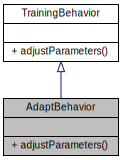
\includegraphics[width=194pt]{class_adapt_behavior__coll__graph}
\end{center}
\end{figure}
\subsection*{Public Member Functions}
\begin{DoxyCompactItemize}
\item 
virtual void \hyperlink{class_adapt_behavior_a718cc9761a139f812db92583b658810b}{adjustParameters} ()=0
\end{DoxyCompactItemize}


\subsection{Detailed Description}
class \hyperlink{class_adapt_behavior}{AdaptBehavior} -\/ 

Definition at line 5 of file AdaptBehavior.h.



\subsection{Member Function Documentation}
\hypertarget{class_adapt_behavior_a718cc9761a139f812db92583b658810b}{
\index{AdaptBehavior@{AdaptBehavior}!adjustParameters@{adjustParameters}}
\index{adjustParameters@{adjustParameters}!AdaptBehavior@{AdaptBehavior}}
\subsubsection[{adjustParameters}]{\setlength{\rightskip}{0pt plus 5cm}virtual void AdaptBehavior::adjustParameters (
\begin{DoxyParamCaption}
{}
\end{DoxyParamCaption}
)\hspace{0.3cm}{\ttfamily  \mbox{[}pure virtual\mbox{]}}}}
\label{class_adapt_behavior_a718cc9761a139f812db92583b658810b}


Reimplemented from \hyperlink{class_training_behavior_ae5729ae35b8557f92872ce778e4d8657}{TrainingBehavior}.



Implemented in \hyperlink{class_a_d_a_p_tgd_a61a992390f1994694918254eb49226a8}{ADAPTgd}, and \hyperlink{class_a_d_a_p_tgdwm_ae7aacd1009a935359982c0b78d87a990}{ADAPTgdwm}.



The documentation for this class was generated from the following file:\begin{DoxyCompactItemize}
\item 
pkg/AMORE/src/dia/\hyperlink{_adapt_behavior_8h}{AdaptBehavior.h}\end{DoxyCompactItemize}

\hypertarget{class_a_d_a_p_tgd}{
\section{ADAPTgd Class Reference}
\label{class_a_d_a_p_tgd}\index{ADAPTgd@{ADAPTgd}}
}


class \hyperlink{class_a_d_a_p_tgd}{ADAPTgd} -\/  




{\ttfamily \#include $<$ADAPTgd.h$>$}



Inheritance diagram for ADAPTgd:
\nopagebreak
\begin{figure}[H]
\begin{center}
\leavevmode
\includegraphics[width=194pt]{class_a_d_a_p_tgd__inherit__graph}
\end{center}
\end{figure}


Collaboration diagram for ADAPTgd:
\nopagebreak
\begin{figure}[H]
\begin{center}
\leavevmode
\includegraphics[width=194pt]{class_a_d_a_p_tgd__coll__graph}
\end{center}
\end{figure}
\subsection*{Public Member Functions}
\begin{DoxyCompactItemize}
\item 
void \hyperlink{class_a_d_a_p_tgd_a61a992390f1994694918254eb49226a8}{adjustParameters} ()
\end{DoxyCompactItemize}
\subsection*{Private Attributes}
\begin{DoxyCompactItemize}
\item 
double \hyperlink{class_a_d_a_p_tgd_a1da50586ed84654472e3c73be57775c6}{outputDerivative}
\end{DoxyCompactItemize}


\subsection{Detailed Description}
class \hyperlink{class_a_d_a_p_tgd}{ADAPTgd} -\/ 

Definition at line 5 of file ADAPTgd.h.



\subsection{Member Function Documentation}
\hypertarget{class_a_d_a_p_tgd_a61a992390f1994694918254eb49226a8}{
\index{ADAPTgd@{ADAPTgd}!adjustParameters@{adjustParameters}}
\index{adjustParameters@{adjustParameters}!ADAPTgd@{ADAPTgd}}
\subsubsection[{adjustParameters}]{\setlength{\rightskip}{0pt plus 5cm}void ADAPTgd::adjustParameters (
\begin{DoxyParamCaption}
{}
\end{DoxyParamCaption}
)\hspace{0.3cm}{\ttfamily  \mbox{[}virtual\mbox{]}}}}
\label{class_a_d_a_p_tgd_a61a992390f1994694918254eb49226a8}


Implements \hyperlink{class_adapt_behavior_a718cc9761a139f812db92583b658810b}{AdaptBehavior}.



\subsection{Member Data Documentation}
\hypertarget{class_a_d_a_p_tgd_a1da50586ed84654472e3c73be57775c6}{
\index{ADAPTgd@{ADAPTgd}!outputDerivative@{outputDerivative}}
\index{outputDerivative@{outputDerivative}!ADAPTgd@{ADAPTgd}}
\subsubsection[{outputDerivative}]{\setlength{\rightskip}{0pt plus 5cm}double {\bf ADAPTgd::outputDerivative}\hspace{0.3cm}{\ttfamily  \mbox{[}private\mbox{]}}}}
\label{class_a_d_a_p_tgd_a1da50586ed84654472e3c73be57775c6}


Definition at line 8 of file ADAPTgd.h.



The documentation for this class was generated from the following file:\begin{DoxyCompactItemize}
\item 
/Users/mcasl/pc-\/ule/Trabajo/investigacion/AMORE/AMORE-\/WC/AMORE-\/WC/pkg/AMORE/src/classHeaders/\hyperlink{_a_d_a_p_tgd_8h}{ADAPTgd.h}\end{DoxyCompactItemize}

\hypertarget{class_a_d_a_p_tgdwm}{
\section{ADAPTgdwm Class Reference}
\label{class_a_d_a_p_tgdwm}\index{ADAPTgdwm@{ADAPTgdwm}}
}


class \hyperlink{class_a_d_a_p_tgdwm}{ADAPTgdwm} -\/  




{\ttfamily \#include $<$ADAPTgdwm.h$>$}



Inheritance diagram for ADAPTgdwm:\nopagebreak
\begin{figure}[H]
\begin{center}
\leavevmode
\includegraphics[width=194pt]{class_a_d_a_p_tgdwm__inherit__graph}
\end{center}
\end{figure}


Collaboration diagram for ADAPTgdwm:\nopagebreak
\begin{figure}[H]
\begin{center}
\leavevmode
\includegraphics[width=194pt]{class_a_d_a_p_tgdwm__coll__graph}
\end{center}
\end{figure}
\subsection*{Public Member Functions}
\begin{DoxyCompactItemize}
\item 
void \hyperlink{class_a_d_a_p_tgdwm_ae7aacd1009a935359982c0b78d87a990}{adjustParameters} ()
\end{DoxyCompactItemize}
\subsection*{Private Attributes}
\begin{DoxyCompactItemize}
\item 
double \hyperlink{class_a_d_a_p_tgdwm_afd8a42a97aff880c902f241e5405abf1}{outputDerivative}
\end{DoxyCompactItemize}


\subsection{Detailed Description}
class \hyperlink{class_a_d_a_p_tgdwm}{ADAPTgdwm} -\/ 

Definition at line 5 of file ADAPTgdwm.h.



\subsection{Member Function Documentation}
\hypertarget{class_a_d_a_p_tgdwm_ae7aacd1009a935359982c0b78d87a990}{
\index{ADAPTgdwm@{ADAPTgdwm}!adjustParameters@{adjustParameters}}
\index{adjustParameters@{adjustParameters}!ADAPTgdwm@{ADAPTgdwm}}
\subsubsection[{adjustParameters}]{\setlength{\rightskip}{0pt plus 5cm}void ADAPTgdwm::adjustParameters (
\begin{DoxyParamCaption}
{}
\end{DoxyParamCaption}
)\hspace{0.3cm}{\ttfamily  \mbox{[}virtual\mbox{]}}}}
\label{class_a_d_a_p_tgdwm_ae7aacd1009a935359982c0b78d87a990}


Implements \hyperlink{class_adapt_behavior_a718cc9761a139f812db92583b658810b}{AdaptBehavior}.



\subsection{Member Data Documentation}
\hypertarget{class_a_d_a_p_tgdwm_afd8a42a97aff880c902f241e5405abf1}{
\index{ADAPTgdwm@{ADAPTgdwm}!outputDerivative@{outputDerivative}}
\index{outputDerivative@{outputDerivative}!ADAPTgdwm@{ADAPTgdwm}}
\subsubsection[{outputDerivative}]{\setlength{\rightskip}{0pt plus 5cm}double {\bf ADAPTgdwm::outputDerivative}\hspace{0.3cm}{\ttfamily  \mbox{[}private\mbox{]}}}}
\label{class_a_d_a_p_tgdwm_afd8a42a97aff880c902f241e5405abf1}


Definition at line 8 of file ADAPTgdwm.h.



The documentation for this class was generated from the following file:\begin{DoxyCompactItemize}
\item 
pkg/AMORE/src/dia/\hyperlink{_a_d_a_p_tgdwm_8h}{ADAPTgdwm.h}\end{DoxyCompactItemize}

\hypertarget{class_batch_behavior}{
\section{BatchBehavior Class Reference}
\label{class_batch_behavior}\index{BatchBehavior@{BatchBehavior}}
}


class \hyperlink{class_batch_behavior}{BatchBehavior} -\/  




{\ttfamily \#include $<$BatchBehavior.h$>$}



Inheritance diagram for BatchBehavior:
\nopagebreak
\begin{figure}[H]
\begin{center}
\leavevmode
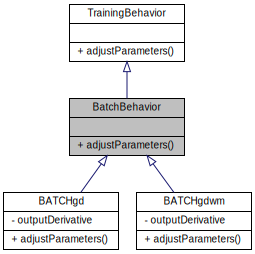
\includegraphics[width=327pt]{class_batch_behavior__inherit__graph}
\end{center}
\end{figure}


Collaboration diagram for BatchBehavior:
\nopagebreak
\begin{figure}[H]
\begin{center}
\leavevmode
\includegraphics[width=194pt]{class_batch_behavior__coll__graph}
\end{center}
\end{figure}
\subsection*{Public Member Functions}
\begin{DoxyCompactItemize}
\item 
virtual void \hyperlink{class_batch_behavior_a491c5129f7f66c6aa6978469338ca41f}{adjustParameters} ()=0
\end{DoxyCompactItemize}


\subsection{Detailed Description}
class \hyperlink{class_batch_behavior}{BatchBehavior} -\/ 

Definition at line 5 of file BatchBehavior.h.



\subsection{Member Function Documentation}
\hypertarget{class_batch_behavior_a491c5129f7f66c6aa6978469338ca41f}{
\index{BatchBehavior@{BatchBehavior}!adjustParameters@{adjustParameters}}
\index{adjustParameters@{adjustParameters}!BatchBehavior@{BatchBehavior}}
\subsubsection[{adjustParameters}]{\setlength{\rightskip}{0pt plus 5cm}virtual void BatchBehavior::adjustParameters (
\begin{DoxyParamCaption}
{}
\end{DoxyParamCaption}
)\hspace{0.3cm}{\ttfamily  \mbox{[}pure virtual\mbox{]}}}}
\label{class_batch_behavior_a491c5129f7f66c6aa6978469338ca41f}


Reimplemented from \hyperlink{class_training_behavior_ae5729ae35b8557f92872ce778e4d8657}{TrainingBehavior}.



Implemented in \hyperlink{class_b_a_t_c_hgd_af595488bdd12a46087edbdab0385251a}{BATCHgd}, and \hyperlink{class_b_a_t_c_hgdwm_af53c2c70dcef41328bb405f2905fd2c9}{BATCHgdwm}.



The documentation for this class was generated from the following file:\begin{DoxyCompactItemize}
\item 
/Users/mcasl/pc-\/ule/Trabajo/investigacion/AMORE/AMORE-\/WC/AMORE-\/WC/pkg/AMORE/src/classHeaders/\hyperlink{_batch_behavior_8h}{BatchBehavior.h}\end{DoxyCompactItemize}

\hypertarget{class_b_a_t_c_hgd}{
\section{BATCHgd Class Reference}
\label{class_b_a_t_c_hgd}\index{BATCHgd@{BATCHgd}}
}


class \hyperlink{class_b_a_t_c_hgd}{BATCHgd} -\/  




{\ttfamily \#include $<$BATCHgd.h$>$}



Inheritance diagram for BATCHgd:
\nopagebreak
\begin{figure}[H]
\begin{center}
\leavevmode
\includegraphics[width=194pt]{class_b_a_t_c_hgd__inherit__graph}
\end{center}
\end{figure}


Collaboration diagram for BATCHgd:
\nopagebreak
\begin{figure}[H]
\begin{center}
\leavevmode
\includegraphics[width=194pt]{class_b_a_t_c_hgd__coll__graph}
\end{center}
\end{figure}
\subsection*{Public Member Functions}
\begin{DoxyCompactItemize}
\item 
void \hyperlink{class_b_a_t_c_hgd_af595488bdd12a46087edbdab0385251a}{adjustParameters} ()
\end{DoxyCompactItemize}
\subsection*{Private Attributes}
\begin{DoxyCompactItemize}
\item 
double \hyperlink{class_b_a_t_c_hgd_a4668a2e34a1323212a71c3aaf378a10d}{outputDerivative}
\end{DoxyCompactItemize}


\subsection{Detailed Description}
class \hyperlink{class_b_a_t_c_hgd}{BATCHgd} -\/ 

Definition at line 5 of file BATCHgd.h.



\subsection{Member Function Documentation}
\hypertarget{class_b_a_t_c_hgd_af595488bdd12a46087edbdab0385251a}{
\index{BATCHgd@{BATCHgd}!adjustParameters@{adjustParameters}}
\index{adjustParameters@{adjustParameters}!BATCHgd@{BATCHgd}}
\subsubsection[{adjustParameters}]{\setlength{\rightskip}{0pt plus 5cm}void BATCHgd::adjustParameters (
\begin{DoxyParamCaption}
{}
\end{DoxyParamCaption}
)\hspace{0.3cm}{\ttfamily  \mbox{[}virtual\mbox{]}}}}
\label{class_b_a_t_c_hgd_af595488bdd12a46087edbdab0385251a}


Implements \hyperlink{class_batch_behavior_a491c5129f7f66c6aa6978469338ca41f}{BatchBehavior}.



\subsection{Member Data Documentation}
\hypertarget{class_b_a_t_c_hgd_a4668a2e34a1323212a71c3aaf378a10d}{
\index{BATCHgd@{BATCHgd}!outputDerivative@{outputDerivative}}
\index{outputDerivative@{outputDerivative}!BATCHgd@{BATCHgd}}
\subsubsection[{outputDerivative}]{\setlength{\rightskip}{0pt plus 5cm}double {\bf BATCHgd::outputDerivative}\hspace{0.3cm}{\ttfamily  \mbox{[}private\mbox{]}}}}
\label{class_b_a_t_c_hgd_a4668a2e34a1323212a71c3aaf378a10d}


Definition at line 8 of file BATCHgd.h.



The documentation for this class was generated from the following file:\begin{DoxyCompactItemize}
\item 
/Users/mcasl/pc-\/ule/Trabajo/investigacion/AMORE/AMORE-\/WC/AMORE-\/WC/pkg/AMORE/src/classHeaders/\hyperlink{_b_a_t_c_hgd_8h}{BATCHgd.h}\end{DoxyCompactItemize}

\hypertarget{class_b_a_t_c_hgdwm}{
\section{BATCHgdwm Class Reference}
\label{class_b_a_t_c_hgdwm}\index{BATCHgdwm@{BATCHgdwm}}
}


class \hyperlink{class_b_a_t_c_hgdwm}{BATCHgdwm} -\/  




{\ttfamily \#include $<$BATCHgdwm.h$>$}



Inheritance diagram for BATCHgdwm:
\nopagebreak
\begin{figure}[H]
\begin{center}
\leavevmode
\includegraphics[width=194pt]{class_b_a_t_c_hgdwm__inherit__graph}
\end{center}
\end{figure}


Collaboration diagram for BATCHgdwm:
\nopagebreak
\begin{figure}[H]
\begin{center}
\leavevmode
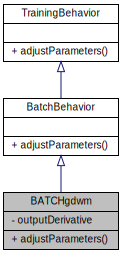
\includegraphics[width=194pt]{class_b_a_t_c_hgdwm__coll__graph}
\end{center}
\end{figure}
\subsection*{Public Member Functions}
\begin{DoxyCompactItemize}
\item 
void \hyperlink{class_b_a_t_c_hgdwm_af53c2c70dcef41328bb405f2905fd2c9}{adjustParameters} ()
\end{DoxyCompactItemize}
\subsection*{Private Attributes}
\begin{DoxyCompactItemize}
\item 
double \hyperlink{class_b_a_t_c_hgdwm_af22fdd2215a316dfe0739d377fcb87a8}{outputDerivative}
\end{DoxyCompactItemize}


\subsection{Detailed Description}
class \hyperlink{class_b_a_t_c_hgdwm}{BATCHgdwm} -\/ 

Definition at line 5 of file BATCHgdwm.h.



\subsection{Member Function Documentation}
\hypertarget{class_b_a_t_c_hgdwm_af53c2c70dcef41328bb405f2905fd2c9}{
\index{BATCHgdwm@{BATCHgdwm}!adjustParameters@{adjustParameters}}
\index{adjustParameters@{adjustParameters}!BATCHgdwm@{BATCHgdwm}}
\subsubsection[{adjustParameters}]{\setlength{\rightskip}{0pt plus 5cm}void BATCHgdwm::adjustParameters (
\begin{DoxyParamCaption}
{}
\end{DoxyParamCaption}
)\hspace{0.3cm}{\ttfamily  \mbox{[}virtual\mbox{]}}}}
\label{class_b_a_t_c_hgdwm_af53c2c70dcef41328bb405f2905fd2c9}


Implements \hyperlink{class_batch_behavior_a491c5129f7f66c6aa6978469338ca41f}{BatchBehavior}.



\subsection{Member Data Documentation}
\hypertarget{class_b_a_t_c_hgdwm_af22fdd2215a316dfe0739d377fcb87a8}{
\index{BATCHgdwm@{BATCHgdwm}!outputDerivative@{outputDerivative}}
\index{outputDerivative@{outputDerivative}!BATCHgdwm@{BATCHgdwm}}
\subsubsection[{outputDerivative}]{\setlength{\rightskip}{0pt plus 5cm}double {\bf BATCHgdwm::outputDerivative}\hspace{0.3cm}{\ttfamily  \mbox{[}private\mbox{]}}}}
\label{class_b_a_t_c_hgdwm_af22fdd2215a316dfe0739d377fcb87a8}


Definition at line 8 of file BATCHgdwm.h.



The documentation for this class was generated from the following file:\begin{DoxyCompactItemize}
\item 
/Users/mcasl/pc-\/ule/Trabajo/investigacion/AMORE/AMORE-\/WC/AMORE-\/WC/pkg/AMORE/src/classHeaders/\hyperlink{_b_a_t_c_hgdwm_8h}{BATCHgdwm.h}\end{DoxyCompactItemize}

\hypertarget{class_con}{
\section{Con Class Reference}
\label{class_con}\index{Con@{Con}}
}


class \hyperlink{class_con}{Con} -\/  




{\ttfamily \#include $<$Con.h$>$}

\subsection*{Public Member Functions}
\begin{DoxyCompactItemize}
\item 
\hyperlink{class_con_a7fab3ece0e894f44f31d10a21b1d49c7}{Con} (\hyperlink{class_neuron}{Neuron} \&neuron)
\begin{DoxyCompactList}\small\item\em Constructor. \end{DoxyCompactList}\item 
\hyperlink{class_con_ad0b1e0d1eefd2296b23a2cfea04fc559}{Con} (\hyperlink{class_neuron}{Neuron} \&neuron, double weight)
\begin{DoxyCompactList}\small\item\em Constructor. \end{DoxyCompactList}\item 
\hyperlink{_a_m_o_r_e_8h_abc871abb71cff6655b8172ee7240b8ef}{Handler} \hyperlink{class_con_aee0a0b6c5beff6e227f9ebf33af2d209}{Id} ()
\begin{DoxyCompactList}\small\item\em A getter of the Id of the \hyperlink{class_neuron}{Neuron} pointed by the from field. \end{DoxyCompactList}\item 
\hyperlink{class_neuron}{Neuron} \& \hyperlink{class_con_a2209567efd330a58825b5068a421afe1}{getNeuron} ()
\begin{DoxyCompactList}\small\item\em from field accessor. \end{DoxyCompactList}\item 
void \hyperlink{class_con_ae372f50a253a424376959fb6ee8f083b}{setNeuron} (\hyperlink{class_neuron}{Neuron} \&neuron)
\item 
double \hyperlink{class_con_a385c5bf6eb9e2ffc94c5b427c287ccb2}{getWeight} ()
\begin{DoxyCompactList}\small\item\em weight field accessor. \end{DoxyCompactList}\item 
void \hyperlink{class_con_acf3b130556e25414cd525d469b275239}{setWeight} (double weight)
\item 
void \hyperlink{class_con_a6fac8dbf2a320d6fb674295a9c900a8a}{show} ()
\begin{DoxyCompactList}\small\item\em Pretty print of the \hyperlink{class_con}{Con} information. \end{DoxyCompactList}\item 
bool \hyperlink{class_con_af5f836a7b0988b3d9113589b2959d5e6}{validate} ()
\begin{DoxyCompactList}\small\item\em Object validator. \end{DoxyCompactList}\end{DoxyCompactItemize}
\subsection*{Private Attributes}
\begin{DoxyCompactItemize}
\item 
\hyperlink{_a_m_o_r_e_8h_ae4f8e0af6c35f16f9f1d3588d8915cf6}{NeuronRef} \hyperlink{class_con_aad857bd289343ecff2153acc852f34f0}{d\_\-neuron}
\item 
double \hyperlink{class_con_a41e043e0dfb126f3bdacbbd8caf33672}{d\_\-weight}
\end{DoxyCompactItemize}


\subsection{Detailed Description}
class \hyperlink{class_con}{Con} -\/ 

Definition at line 3 of file Con.h.



\subsection{Constructor \& Destructor Documentation}
\hypertarget{class_con_a7fab3ece0e894f44f31d10a21b1d49c7}{
\index{Con@{Con}!Con@{Con}}
\index{Con@{Con}!Con@{Con}}
\subsubsection[{Con}]{\setlength{\rightskip}{0pt plus 5cm}Con::Con (
\begin{DoxyParamCaption}
\item[{{\bf Neuron} \&}]{neuron}
\end{DoxyParamCaption}
)}}
\label{class_con_a7fab3ece0e894f44f31d10a21b1d49c7}


Constructor. 



Definition at line 19 of file Con.cpp.


\begin{DoxyCode}
                       :
  d_neuron( boost::ref(neuron) ), d_weight(0)
{
}
\end{DoxyCode}
\hypertarget{class_con_ad0b1e0d1eefd2296b23a2cfea04fc559}{
\index{Con@{Con}!Con@{Con}}
\index{Con@{Con}!Con@{Con}}
\subsubsection[{Con}]{\setlength{\rightskip}{0pt plus 5cm}Con::Con (
\begin{DoxyParamCaption}
\item[{{\bf Neuron} \&}]{neuron, }
\item[{double}]{weight}
\end{DoxyParamCaption}
)}}
\label{class_con_ad0b1e0d1eefd2296b23a2cfea04fc559}


Constructor. 



Definition at line 30 of file Con.cpp.


\begin{DoxyCode}
                                      :
  d_neuron(boost::ref(neuron)), d_weight(weight)
{
}
\end{DoxyCode}


\subsection{Member Function Documentation}
\hypertarget{class_con_a2209567efd330a58825b5068a421afe1}{
\index{Con@{Con}!getNeuron@{getNeuron}}
\index{getNeuron@{getNeuron}!Con@{Con}}
\subsubsection[{getNeuron}]{\setlength{\rightskip}{0pt plus 5cm}{\bf Neuron} \& Con::getNeuron (
\begin{DoxyParamCaption}
{}
\end{DoxyParamCaption}
)}}
\label{class_con_a2209567efd330a58825b5068a421afe1}


from field accessor. 

This method allows access to the address stored in the private from field (a pointer to a \hyperlink{class_neuron}{Neuron} object).$\ast$ \begin{DoxyReturn}{Returns}
A pointer to the \hyperlink{class_neuron}{Neuron} object referred to by the from field.
\end{DoxyReturn}

\begin{DoxyCode}
        //================
        //Usage example:
        //================
        // Data set up
                        NeuronPtr ptShNeuron ( new Neuron(1) );         // Neuron
       Id is set 1
                        ConPtr ptShCon( new Con(ptShNeuron) );          // from p
      oints to ptShNeuron and weight is set to 0
        // Test
                        ptShNeuron = ptShCon->getFrom() ;
                        int result = ptShNeuron->getId();

        // Now, result is equal to 1.
\end{DoxyCode}


\begin{DoxySeeAlso}{See also}
getId and the unit test files, e.g., runit.Cpp.Con.R, for further examples. 
\end{DoxySeeAlso}


Definition at line 56 of file Con.cpp.



References d\_\-neuron.


\begin{DoxyCode}
{
  return d_neuron;
}
\end{DoxyCode}
\hypertarget{class_con_a385c5bf6eb9e2ffc94c5b427c287ccb2}{
\index{Con@{Con}!getWeight@{getWeight}}
\index{getWeight@{getWeight}!Con@{Con}}
\subsubsection[{getWeight}]{\setlength{\rightskip}{0pt plus 5cm}double Con::getWeight (
\begin{DoxyParamCaption}
{}
\end{DoxyParamCaption}
)}}
\label{class_con_a385c5bf6eb9e2ffc94c5b427c287ccb2}


weight field accessor. 

This method allows access to the value stored in the private field weight \begin{DoxyReturn}{Returns}
The value of weight (double)
\end{DoxyReturn}

\begin{DoxyCode}
  //================
  //Usage example:
  //================
  // Data set up
                        std::vector<double> result;
                        NeuronPtr ptShNeuron ( new Neuron(16) );                /
      / Neuron Id is set to 16
                        ConPtr ptShCon( new Con(ptShNeuron, 12.4) );  // from poi
      nts to ptShNeuron and weight is set to 12.4
        // Test
                        result.push_back( ptShCon->getWeight() );
                        ptShCon->setWeight(2.2);
                        result.push_back( ptShCon->getWeight() );

        // Now, result is a numeric vector that contains the values 12.4 and 2.2 
      .
\end{DoxyCode}


\begin{DoxySeeAlso}{See also}
\hyperlink{class_con_acf3b130556e25414cd525d469b275239}{setWeight} and the unit test files, e.g., runit.Cpp.Con.R, for further examples. 
\end{DoxySeeAlso}


Definition at line 116 of file Con.cpp.



References d\_\-weight.



Referenced by show(), and validate().


\begin{DoxyCode}
{
  return d_weight;
}
\end{DoxyCode}


Here is the caller graph for this function:
\nopagebreak
\begin{figure}[H]
\begin{center}
\leavevmode
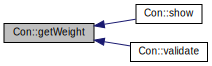
\includegraphics[width=284pt]{class_con_a385c5bf6eb9e2ffc94c5b427c287ccb2_icgraph}
\end{center}
\end{figure}


\hypertarget{class_con_aee0a0b6c5beff6e227f9ebf33af2d209}{
\index{Con@{Con}!Id@{Id}}
\index{Id@{Id}!Con@{Con}}
\subsubsection[{Id}]{\setlength{\rightskip}{0pt plus 5cm}int Con::Id (
\begin{DoxyParamCaption}
{}
\end{DoxyParamCaption}
)}}
\label{class_con_aee0a0b6c5beff6e227f9ebf33af2d209}


A getter of the Id of the \hyperlink{class_neuron}{Neuron} pointed by the from field. 

This method gets the Id of the \hyperlink{class_neuron}{Neuron} referred to by the from field \begin{DoxyReturn}{Returns}
The value of the Id (an integer).
\end{DoxyReturn}

\begin{DoxyCode}
      //================
      //Usage example:
      //================
      // Data set up
                      NeuronPtr ptShNeuron ( new Neuron(16) );        // Neuron I
      d is set to 16
                      ConPtr ptShCon( new Con(ptShNeuron) );          // from poi
      nts to ptShNeuron and weight is set to 0
      // Test
                      int result = ptShCon->getId();

      // Now, result is equal to 16.
\end{DoxyCode}


\begin{DoxySeeAlso}{See also}
getFrom, setFrom and the unit test files, e.g., runit.Cpp.Con.R, for further examples. 
\end{DoxySeeAlso}


Definition at line 88 of file Con.cpp.



References d\_\-neuron.



Referenced by show(), and validate().


\begin{DoxyCode}
{
  return d_neuron.get().getId();
}
\end{DoxyCode}


Here is the caller graph for this function:
\nopagebreak
\begin{figure}[H]
\begin{center}
\leavevmode
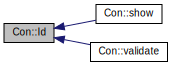
\includegraphics[width=244pt]{class_con_aee0a0b6c5beff6e227f9ebf33af2d209_icgraph}
\end{center}
\end{figure}


\hypertarget{class_con_ae372f50a253a424376959fb6ee8f083b}{
\index{Con@{Con}!setNeuron@{setNeuron}}
\index{setNeuron@{setNeuron}!Con@{Con}}
\subsubsection[{setNeuron}]{\setlength{\rightskip}{0pt plus 5cm}void Con::setNeuron (
\begin{DoxyParamCaption}
\item[{{\bf Neuron} \&}]{neuron}
\end{DoxyParamCaption}
)}}
\label{class_con_ae372f50a253a424376959fb6ee8f083b}


Definition at line 63 of file Con.cpp.



References d\_\-neuron.


\begin{DoxyCode}
{
  d_neuron=boost::ref(neuron);
}
\end{DoxyCode}
\hypertarget{class_con_acf3b130556e25414cd525d469b275239}{
\index{Con@{Con}!setWeight@{setWeight}}
\index{setWeight@{setWeight}!Con@{Con}}
\subsubsection[{setWeight}]{\setlength{\rightskip}{0pt plus 5cm}void Con::setWeight (
\begin{DoxyParamCaption}
\item[{double}]{weight}
\end{DoxyParamCaption}
)}}
\label{class_con_acf3b130556e25414cd525d469b275239}


Definition at line 123 of file Con.cpp.



References d\_\-weight.


\begin{DoxyCode}
{
  d_weight=weight;
}
\end{DoxyCode}
\hypertarget{class_con_a6fac8dbf2a320d6fb674295a9c900a8a}{
\index{Con@{Con}!show@{show}}
\index{show@{show}!Con@{Con}}
\subsubsection[{show}]{\setlength{\rightskip}{0pt plus 5cm}void Con::show (
\begin{DoxyParamCaption}
{}
\end{DoxyParamCaption}
)}}
\label{class_con_a6fac8dbf2a320d6fb674295a9c900a8a}


Pretty print of the \hyperlink{class_con}{Con} information. 

This method outputs in the R terminal the contents of the \hyperlink{class_con}{Con} fields. \begin{DoxyReturn}{Returns}
true in case everything works without throwing an exception 
\end{DoxyReturn}
\begin{DoxySeeAlso}{See also}
\hyperlink{class_con_acf3b130556e25414cd525d469b275239}{setWeight} and the unit test files, e.g., runit.Cpp.Con.R, for usage examples. 
\end{DoxySeeAlso}


Definition at line 135 of file Con.cpp.



References getWeight(), and Id().


\begin{DoxyCode}
{
  int id = Id();
  if (id == NA_INTEGER)
    {
      Rprintf("From: NA\t Invalid Connection \n");
    }
  else
    {
      Rprintf("From:\t %d \t Weight= \t %lf \n", id , getWeight() );
    }
}
\end{DoxyCode}


Here is the call graph for this function:
\nopagebreak
\begin{figure}[H]
\begin{center}
\leavevmode
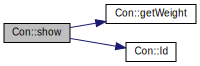
\includegraphics[width=272pt]{class_con_a6fac8dbf2a320d6fb674295a9c900a8a_cgraph}
\end{center}
\end{figure}


\hypertarget{class_con_af5f836a7b0988b3d9113589b2959d5e6}{
\index{Con@{Con}!validate@{validate}}
\index{validate@{validate}!Con@{Con}}
\subsubsection[{validate}]{\setlength{\rightskip}{0pt plus 5cm}bool Con::validate (
\begin{DoxyParamCaption}
{}
\end{DoxyParamCaption}
)}}
\label{class_con_af5f836a7b0988b3d9113589b2959d5e6}


Object validator. 

This method checks the object for internal coherence. A try / catch mechanism exits normal execution and returns control to the R terminal in case the contents of the \hyperlink{class_con}{Con} object are identified as corrupted. \begin{DoxyReturn}{Returns}
true in case the checks are Ok. 
\end{DoxyReturn}

\begin{DoxyExceptions}{Exceptions}
{\em An} & std::range error if weight or from are not finite. \\
\hline
\end{DoxyExceptions}


Definition at line 155 of file Con.cpp.



References getWeight(), and Id().


\begin{DoxyCode}
{
  BEGIN_RCPP
  if (! R_FINITE(getWeight()) ) throw std::range_error("weight is not finite.");
  if (Id() == NA_INTEGER)
    throw std::range_error("fromId is not finite.");
  return (true);
END_RCPP}
\end{DoxyCode}


Here is the call graph for this function:\nopagebreak
\begin{figure}[H]
\begin{center}
\leavevmode
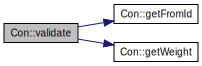
\includegraphics[width=284pt]{class_con_af5f836a7b0988b3d9113589b2959d5e6_cgraph}
\end{center}
\end{figure}




\subsection{Member Data Documentation}
\hypertarget{class_con_aad857bd289343ecff2153acc852f34f0}{
\index{Con@{Con}!d\_\-neuron@{d\_\-neuron}}
\index{d\_\-neuron@{d\_\-neuron}!Con@{Con}}
\subsubsection[{d\_\-neuron}]{\setlength{\rightskip}{0pt plus 5cm}{\bf NeuronRef} {\bf Con::d\_\-neuron}\hspace{0.3cm}{\ttfamily  \mbox{[}private\mbox{]}}}}
\label{class_con_aad857bd289343ecff2153acc852f34f0}


Definition at line 6 of file Con.h.



Referenced by getNeuron(), Id(), and setNeuron().

\hypertarget{class_con_a41e043e0dfb126f3bdacbbd8caf33672}{
\index{Con@{Con}!d\_\-weight@{d\_\-weight}}
\index{d\_\-weight@{d\_\-weight}!Con@{Con}}
\subsubsection[{d\_\-weight}]{\setlength{\rightskip}{0pt plus 5cm}double {\bf Con::d\_\-weight}\hspace{0.3cm}{\ttfamily  \mbox{[}private\mbox{]}}}}
\label{class_con_a41e043e0dfb126f3bdacbbd8caf33672}


Definition at line 7 of file Con.h.



Referenced by getWeight(), and setWeight().



The documentation for this class was generated from the following files:\begin{DoxyCompactItemize}
\item 
pkg/AMORE/src/dia/\hyperlink{_con_8h}{Con.h}\item 
pkg/AMORE/src/\hyperlink{_con_8cpp}{Con.cpp}\end{DoxyCompactItemize}

\hypertarget{class_container}{
\section{Container$<$ T $>$ Class Template Reference}
\label{class_container}\index{Container@{Container}}
}


class \hyperlink{class_container}{Container} -\/  




{\ttfamily \#include $<$Container.h$>$}



Inheritance diagram for Container$<$ T $>$:
\nopagebreak
\begin{figure}[H]
\begin{center}
\leavevmode
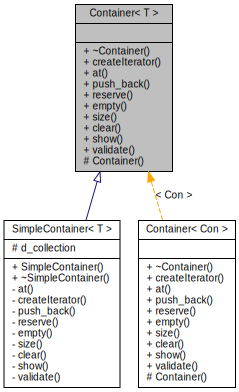
\includegraphics[width=196pt]{class_container__inherit__graph}
\end{center}
\end{figure}
\subsection*{Public Member Functions}
\begin{DoxyCompactItemize}
\item 
virtual \hyperlink{class_container_ac190e8e99e5a92ef02390027765cbbb6}{$\sim$Container} ()
\item 
virtual boost::shared\_\-ptr$<$ \hyperlink{class_iterator}{Iterator}$<$ T $>$ $>$ \hyperlink{class_container_a18a0a70153781d3d94526bc09fcbedb8}{createIterator} ()=0
\item 
virtual T \hyperlink{class_container_a8aed06783f7cd0749f796c64e64626e7}{at} (size\_\-type element)=0
\item 
virtual void \hyperlink{class_container_a12ffe2d2dbbcd78b6b293756004bd6e0}{push\_\-back} (T const \&const\_\-reference)=0
\item 
virtual void \hyperlink{class_container_a5f70fb0d821a8db9a0733aafe9ef35ac}{reserve} (int n)=0
\item 
virtual bool \hyperlink{class_container_a123dcd25b363ab92ac8bfa8b4c4061a4}{empty} ()=0
\item 
virtual size\_\-type \hyperlink{class_container_a1eebc7b5cbb0c574cb1aef87c2ddba36}{size} ()=0
\item 
virtual void \hyperlink{class_container_ac27f3554d6ac6ecb227ead060ff1f8a2}{clear} ()=0
\item 
virtual void \hyperlink{class_container_a5ee85af656e60863a7e4c1f7f9c484f4}{show} ()=0
\item 
virtual bool \hyperlink{class_container_abbd8ca2714a550351442f4410cf5736d}{validate} ()=0
\end{DoxyCompactItemize}
\subsection*{Protected Member Functions}
\begin{DoxyCompactItemize}
\item 
\hyperlink{class_container_ab17ce1f67243b28abcd4c8113a72524c}{Container} ()
\end{DoxyCompactItemize}


\subsection{Detailed Description}
\subsubsection*{template$<$typename T$>$class Container$<$ T $>$}

class \hyperlink{class_container}{Container} -\/ 

Definition at line 5 of file Container.h.



\subsection{Constructor \& Destructor Documentation}
\hypertarget{class_container_ac190e8e99e5a92ef02390027765cbbb6}{
\index{Container@{Container}!$\sim$Container@{$\sim$Container}}
\index{$\sim$Container@{$\sim$Container}!Container@{Container}}
\subsubsection[{$\sim$Container}]{\setlength{\rightskip}{0pt plus 5cm}template$<$typename T $>$ virtual {\bf Container}$<$ T $>$::$\sim${\bf Container} (
\begin{DoxyParamCaption}
{}
\end{DoxyParamCaption}
)\hspace{0.3cm}{\ttfamily  \mbox{[}virtual\mbox{]}}}}
\label{class_container_ac190e8e99e5a92ef02390027765cbbb6}
\hypertarget{class_container_ab17ce1f67243b28abcd4c8113a72524c}{
\index{Container@{Container}!Container@{Container}}
\index{Container@{Container}!Container@{Container}}
\subsubsection[{Container}]{\setlength{\rightskip}{0pt plus 5cm}template$<$typename T $>$ {\bf Container}$<$ T $>$::{\bf Container} (
\begin{DoxyParamCaption}
{}
\end{DoxyParamCaption}
)\hspace{0.3cm}{\ttfamily  \mbox{[}protected\mbox{]}}}}
\label{class_container_ab17ce1f67243b28abcd4c8113a72524c}


\subsection{Member Function Documentation}
\hypertarget{class_container_a8aed06783f7cd0749f796c64e64626e7}{
\index{Container@{Container}!at@{at}}
\index{at@{at}!Container@{Container}}
\subsubsection[{at}]{\setlength{\rightskip}{0pt plus 5cm}template$<$typename T $>$ virtual T {\bf Container}$<$ T $>$::at (
\begin{DoxyParamCaption}
\item[{size\_\-type}]{element}
\end{DoxyParamCaption}
)\hspace{0.3cm}{\ttfamily  \mbox{[}pure virtual\mbox{]}}}}
\label{class_container_a8aed06783f7cd0749f796c64e64626e7}


Implemented in \hyperlink{class_simple_container_a2e8f56f3af1e0ffb1fcd54d05d82c477}{SimpleContainer$<$ T $>$}.

\hypertarget{class_container_ac27f3554d6ac6ecb227ead060ff1f8a2}{
\index{Container@{Container}!clear@{clear}}
\index{clear@{clear}!Container@{Container}}
\subsubsection[{clear}]{\setlength{\rightskip}{0pt plus 5cm}template$<$typename T $>$ virtual void {\bf Container}$<$ T $>$::clear (
\begin{DoxyParamCaption}
{}
\end{DoxyParamCaption}
)\hspace{0.3cm}{\ttfamily  \mbox{[}pure virtual\mbox{]}}}}
\label{class_container_ac27f3554d6ac6ecb227ead060ff1f8a2}


Implemented in \hyperlink{class_simple_container_ae3ee6cb18f1dd33ab5de4f9854ce245f}{SimpleContainer$<$ T $>$}.

\hypertarget{class_container_a18a0a70153781d3d94526bc09fcbedb8}{
\index{Container@{Container}!createIterator@{createIterator}}
\index{createIterator@{createIterator}!Container@{Container}}
\subsubsection[{createIterator}]{\setlength{\rightskip}{0pt plus 5cm}template$<$typename T $>$ virtual boost::shared\_\-ptr$<$ {\bf Iterator}$<$T$>$ $>$ {\bf Container}$<$ T $>$::createIterator (
\begin{DoxyParamCaption}
{}
\end{DoxyParamCaption}
)\hspace{0.3cm}{\ttfamily  \mbox{[}pure virtual\mbox{]}}}}
\label{class_container_a18a0a70153781d3d94526bc09fcbedb8}


Implemented in \hyperlink{class_simple_container_a4e46f5cb32231deaf9aa9bb7f871d09e}{SimpleContainer$<$ T $>$}.

\hypertarget{class_container_a123dcd25b363ab92ac8bfa8b4c4061a4}{
\index{Container@{Container}!empty@{empty}}
\index{empty@{empty}!Container@{Container}}
\subsubsection[{empty}]{\setlength{\rightskip}{0pt plus 5cm}template$<$typename T $>$ virtual bool {\bf Container}$<$ T $>$::empty (
\begin{DoxyParamCaption}
{}
\end{DoxyParamCaption}
)\hspace{0.3cm}{\ttfamily  \mbox{[}pure virtual\mbox{]}}}}
\label{class_container_a123dcd25b363ab92ac8bfa8b4c4061a4}


Implemented in \hyperlink{class_simple_container_ac2966f33796f69c290a84361a578ed08}{SimpleContainer$<$ T $>$}.

\hypertarget{class_container_a12ffe2d2dbbcd78b6b293756004bd6e0}{
\index{Container@{Container}!push\_\-back@{push\_\-back}}
\index{push\_\-back@{push\_\-back}!Container@{Container}}
\subsubsection[{push\_\-back}]{\setlength{\rightskip}{0pt plus 5cm}template$<$typename T $>$ virtual void {\bf Container}$<$ T $>$::push\_\-back (
\begin{DoxyParamCaption}
\item[{T const \&}]{const\_\-reference}
\end{DoxyParamCaption}
)\hspace{0.3cm}{\ttfamily  \mbox{[}pure virtual\mbox{]}}}}
\label{class_container_a12ffe2d2dbbcd78b6b293756004bd6e0}


Implemented in \hyperlink{class_simple_container_a53466966297b3f0a707e025b3721004a}{SimpleContainer$<$ T $>$}.

\hypertarget{class_container_a5f70fb0d821a8db9a0733aafe9ef35ac}{
\index{Container@{Container}!reserve@{reserve}}
\index{reserve@{reserve}!Container@{Container}}
\subsubsection[{reserve}]{\setlength{\rightskip}{0pt plus 5cm}template$<$typename T $>$ virtual void {\bf Container}$<$ T $>$::reserve (
\begin{DoxyParamCaption}
\item[{int}]{n}
\end{DoxyParamCaption}
)\hspace{0.3cm}{\ttfamily  \mbox{[}pure virtual\mbox{]}}}}
\label{class_container_a5f70fb0d821a8db9a0733aafe9ef35ac}


Implemented in \hyperlink{class_simple_container_a4bca44e6a9cef9d57627218c0a180d8a}{SimpleContainer$<$ T $>$}.

\hypertarget{class_container_a5ee85af656e60863a7e4c1f7f9c484f4}{
\index{Container@{Container}!show@{show}}
\index{show@{show}!Container@{Container}}
\subsubsection[{show}]{\setlength{\rightskip}{0pt plus 5cm}template$<$typename T $>$ virtual void {\bf Container}$<$ T $>$::show (
\begin{DoxyParamCaption}
{}
\end{DoxyParamCaption}
)\hspace{0.3cm}{\ttfamily  \mbox{[}pure virtual\mbox{]}}}}
\label{class_container_a5ee85af656e60863a7e4c1f7f9c484f4}


Implemented in \hyperlink{class_simple_container_af4d591e2c3a44ae016e01e3d07d1e9ac}{SimpleContainer$<$ T $>$}.

\hypertarget{class_container_a1eebc7b5cbb0c574cb1aef87c2ddba36}{
\index{Container@{Container}!size@{size}}
\index{size@{size}!Container@{Container}}
\subsubsection[{size}]{\setlength{\rightskip}{0pt plus 5cm}template$<$typename T $>$ virtual size\_\-type {\bf Container}$<$ T $>$::size (
\begin{DoxyParamCaption}
{}
\end{DoxyParamCaption}
)\hspace{0.3cm}{\ttfamily  \mbox{[}pure virtual\mbox{]}}}}
\label{class_container_a1eebc7b5cbb0c574cb1aef87c2ddba36}


Implemented in \hyperlink{class_simple_container_a2fdb3580e1728e6e2ba6ef77c0bce63e}{SimpleContainer$<$ T $>$}.

\hypertarget{class_container_abbd8ca2714a550351442f4410cf5736d}{
\index{Container@{Container}!validate@{validate}}
\index{validate@{validate}!Container@{Container}}
\subsubsection[{validate}]{\setlength{\rightskip}{0pt plus 5cm}template$<$typename T $>$ virtual bool {\bf Container}$<$ T $>$::validate (
\begin{DoxyParamCaption}
{}
\end{DoxyParamCaption}
)\hspace{0.3cm}{\ttfamily  \mbox{[}pure virtual\mbox{]}}}}
\label{class_container_abbd8ca2714a550351442f4410cf5736d}


Implemented in \hyperlink{class_simple_container_ac7cae8eaac2dc0a69138b65f679bd16a}{SimpleContainer$<$ T $>$}.



The documentation for this class was generated from the following file:\begin{DoxyCompactItemize}
\item 
/Users/mcasl/pc-\/ule/Trabajo/investigacion/AMORE/AMORE-\/WC/AMORE-\/WC/pkg/AMORE/src/classHeaders/\hyperlink{_container_8h}{Container.h}\end{DoxyCompactItemize}

\hypertarget{class_iterator}{
\section{Iterator$<$ T $>$ Class Template Reference}
\label{class_iterator}\index{Iterator@{Iterator}}
}


class \hyperlink{class_iterator}{Iterator} -\/  




{\ttfamily \#include $<$Iterator.h$>$}



Inheritance diagram for Iterator$<$ T $>$:
\nopagebreak
\begin{figure}[H]
\begin{center}
\leavevmode
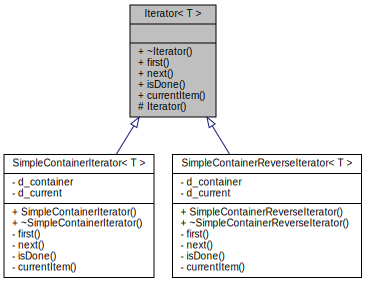
\includegraphics[width=400pt]{class_iterator__inherit__graph}
\end{center}
\end{figure}
\subsection*{Public Member Functions}
\begin{DoxyCompactItemize}
\item 
virtual \hyperlink{class_iterator_a9e5aab5b020f674497ee9752ab31db8a}{$\sim$Iterator} ()
\item 
virtual void \hyperlink{class_iterator_a6f13cc79a1574086c63ce4ddba1d3d9f}{first} ()=0
\item 
virtual void \hyperlink{class_iterator_a94a7b0c50676cd9ee924eddece41d8d4}{next} ()=0
\item 
virtual bool \hyperlink{class_iterator_a8e7b414c641f4f0838ff8bd6ba954b7a}{isDone} ()=0
\item 
virtual T \hyperlink{class_iterator_a1fce5bc9b2218407b5cedf2a0ba3131b}{currentItem} ()=0
\end{DoxyCompactItemize}
\subsection*{Protected Member Functions}
\begin{DoxyCompactItemize}
\item 
\hyperlink{class_iterator_a87d4af70ba6312e91e1ab6a7c9e2ec6d}{Iterator} ()
\end{DoxyCompactItemize}


\subsection{Detailed Description}
\subsubsection*{template$<$typename T$>$class Iterator$<$ T $>$}

class \hyperlink{class_iterator}{Iterator} -\/ 

Definition at line 5 of file Iterator.h.



\subsection{Constructor \& Destructor Documentation}
\hypertarget{class_iterator_a9e5aab5b020f674497ee9752ab31db8a}{
\index{Iterator@{Iterator}!$\sim$Iterator@{$\sim$Iterator}}
\index{$\sim$Iterator@{$\sim$Iterator}!Iterator@{Iterator}}
\subsubsection[{$\sim$Iterator}]{\setlength{\rightskip}{0pt plus 5cm}template$<$typename T $>$ virtual {\bf Iterator}$<$ T $>$::$\sim${\bf Iterator} (
\begin{DoxyParamCaption}
{}
\end{DoxyParamCaption}
)\hspace{0.3cm}{\ttfamily  \mbox{[}virtual\mbox{]}}}}
\label{class_iterator_a9e5aab5b020f674497ee9752ab31db8a}
\hypertarget{class_iterator_a87d4af70ba6312e91e1ab6a7c9e2ec6d}{
\index{Iterator@{Iterator}!Iterator@{Iterator}}
\index{Iterator@{Iterator}!Iterator@{Iterator}}
\subsubsection[{Iterator}]{\setlength{\rightskip}{0pt plus 5cm}template$<$typename T $>$ {\bf Iterator}$<$ T $>$::{\bf Iterator} (
\begin{DoxyParamCaption}
{}
\end{DoxyParamCaption}
)\hspace{0.3cm}{\ttfamily  \mbox{[}protected\mbox{]}}}}
\label{class_iterator_a87d4af70ba6312e91e1ab6a7c9e2ec6d}


\subsection{Member Function Documentation}
\hypertarget{class_iterator_a1fce5bc9b2218407b5cedf2a0ba3131b}{
\index{Iterator@{Iterator}!currentItem@{currentItem}}
\index{currentItem@{currentItem}!Iterator@{Iterator}}
\subsubsection[{currentItem}]{\setlength{\rightskip}{0pt plus 5cm}template$<$typename T $>$ virtual T {\bf Iterator}$<$ T $>$::currentItem (
\begin{DoxyParamCaption}
{}
\end{DoxyParamCaption}
)\hspace{0.3cm}{\ttfamily  \mbox{[}pure virtual\mbox{]}}}}
\label{class_iterator_a1fce5bc9b2218407b5cedf2a0ba3131b}


Implemented in \hyperlink{class_simple_container_iterator_ad65642e6d9540b58193e7a40f1688fc7}{SimpleContainerIterator$<$ T $>$}, and \hyperlink{class_simple_container_reverse_iterator_a5930732e1d179eeccbbfd44f0287eecb}{SimpleContainerReverseIterator$<$ T $>$}.

\hypertarget{class_iterator_a6f13cc79a1574086c63ce4ddba1d3d9f}{
\index{Iterator@{Iterator}!first@{first}}
\index{first@{first}!Iterator@{Iterator}}
\subsubsection[{first}]{\setlength{\rightskip}{0pt plus 5cm}template$<$typename T $>$ virtual void {\bf Iterator}$<$ T $>$::first (
\begin{DoxyParamCaption}
{}
\end{DoxyParamCaption}
)\hspace{0.3cm}{\ttfamily  \mbox{[}pure virtual\mbox{]}}}}
\label{class_iterator_a6f13cc79a1574086c63ce4ddba1d3d9f}


Implemented in \hyperlink{class_simple_container_iterator_a71b26d5acddcab75ca0386c187fd2bbc}{SimpleContainerIterator$<$ T $>$}, and \hyperlink{class_simple_container_reverse_iterator_a668e22d824eca8ec3cb3a49765012c52}{SimpleContainerReverseIterator$<$ T $>$}.

\hypertarget{class_iterator_a8e7b414c641f4f0838ff8bd6ba954b7a}{
\index{Iterator@{Iterator}!isDone@{isDone}}
\index{isDone@{isDone}!Iterator@{Iterator}}
\subsubsection[{isDone}]{\setlength{\rightskip}{0pt plus 5cm}template$<$typename T $>$ virtual bool {\bf Iterator}$<$ T $>$::isDone (
\begin{DoxyParamCaption}
{}
\end{DoxyParamCaption}
)\hspace{0.3cm}{\ttfamily  \mbox{[}pure virtual\mbox{]}}}}
\label{class_iterator_a8e7b414c641f4f0838ff8bd6ba954b7a}


Implemented in \hyperlink{class_simple_container_iterator_a91352e803f39fb58d9312d9d866842c8}{SimpleContainerIterator$<$ T $>$}, and \hyperlink{class_simple_container_reverse_iterator_aaad6fe33e00ead55155f42bfbbe8ea04}{SimpleContainerReverseIterator$<$ T $>$}.

\hypertarget{class_iterator_a94a7b0c50676cd9ee924eddece41d8d4}{
\index{Iterator@{Iterator}!next@{next}}
\index{next@{next}!Iterator@{Iterator}}
\subsubsection[{next}]{\setlength{\rightskip}{0pt plus 5cm}template$<$typename T $>$ virtual void {\bf Iterator}$<$ T $>$::next (
\begin{DoxyParamCaption}
{}
\end{DoxyParamCaption}
)\hspace{0.3cm}{\ttfamily  \mbox{[}pure virtual\mbox{]}}}}
\label{class_iterator_a94a7b0c50676cd9ee924eddece41d8d4}


Implemented in \hyperlink{class_simple_container_iterator_a11274af2bc4dc9930f983b7b246d8f87}{SimpleContainerIterator$<$ T $>$}, and \hyperlink{class_simple_container_reverse_iterator_a21346e891b30bd217d7ca5aa51622dbe}{SimpleContainerReverseIterator$<$ T $>$}.



The documentation for this class was generated from the following file:\begin{DoxyCompactItemize}
\item 
/Users/mcasl/pc-\/ule/Trabajo/investigacion/AMORE/AMORE-\/WC/AMORE-\/WC/pkg/AMORE/src/classHeaders/\hyperlink{_iterator_8h}{Iterator.h}\end{DoxyCompactItemize}

\hypertarget{class_m_l_pbehavior}{
\section{MLPbehavior Class Reference}
\label{class_m_l_pbehavior}\index{MLPbehavior@{MLPbehavior}}
}


class \hyperlink{class_m_l_pbehavior}{MLPbehavior} -\/  




{\ttfamily \#include $<$MLPbehavior.h$>$}



Inheritance diagram for MLPbehavior:
\nopagebreak
\begin{figure}[H]
\begin{center}
\leavevmode
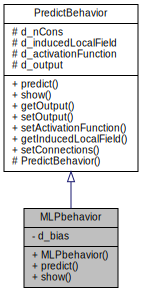
\includegraphics[width=170pt]{class_m_l_pbehavior__inherit__graph}
\end{center}
\end{figure}


Collaboration diagram for MLPbehavior:
\nopagebreak
\begin{figure}[H]
\begin{center}
\leavevmode
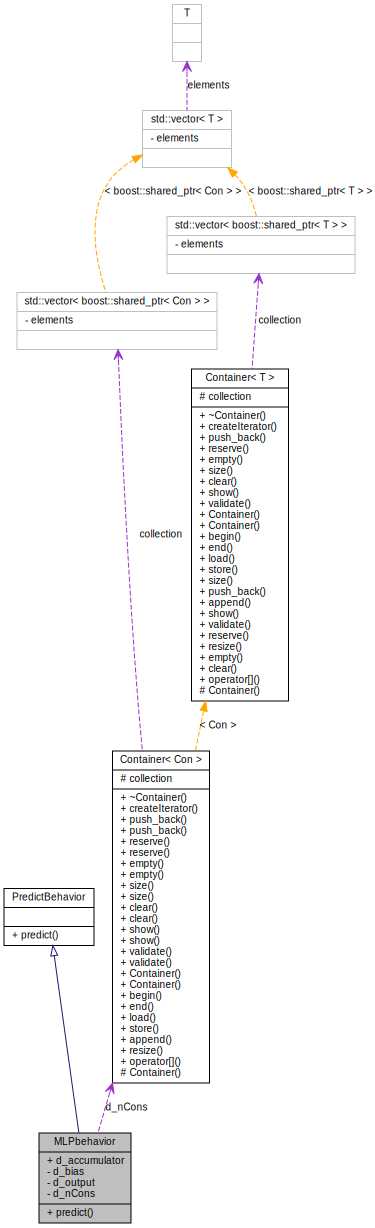
\includegraphics[width=170pt]{class_m_l_pbehavior__coll__graph}
\end{center}
\end{figure}
\subsection*{Public Member Functions}
\begin{DoxyCompactItemize}
\item 
void \hyperlink{class_m_l_pbehavior_aaff94adc3577cda9e48d8da925b0ffbf}{predict} ()
\item 
void \hyperlink{class_m_l_pbehavior_a32aa885e07e8f4eb33e05afb46040567}{show} ()
\end{DoxyCompactItemize}
\subsection*{Private Attributes}
\begin{DoxyCompactItemize}
\item 
double \hyperlink{class_m_l_pbehavior_a6206785c5c3f838a0538f9f77fa7a25a}{d\_\-bias}
\item 
double \hyperlink{class_m_l_pbehavior_a1a2045f66e72cd110227735ac0930900}{d\_\-output}
\item 
\hyperlink{_a_m_o_r_e_8h_a1021dbaf961d1c8da6d58a8566e5778b}{ConContainerPtr} \hyperlink{class_m_l_pbehavior_acb6e9681f06195ba1dd63bbafaa51d68}{d\_\-nCons}
\item 
double \hyperlink{class_m_l_pbehavior_a5e3dcaba201554283d27d58c6aa3ea82}{d\_\-accumulator}
\end{DoxyCompactItemize}
\subsection*{Friends}
\begin{DoxyCompactItemize}
\item 
class \hyperlink{class_m_l_pbehavior_a1aa48940238b9487734e590ffab33a1b}{MLPfactory}
\end{DoxyCompactItemize}


\subsection{Detailed Description}
class \hyperlink{class_m_l_pbehavior}{MLPbehavior} -\/ 

Definition at line 5 of file MLPbehavior.h.



\subsection{Member Function Documentation}
\hypertarget{class_m_l_pbehavior_aaff94adc3577cda9e48d8da925b0ffbf}{
\index{MLPbehavior@{MLPbehavior}!predict@{predict}}
\index{predict@{predict}!MLPbehavior@{MLPbehavior}}
\subsubsection[{predict}]{\setlength{\rightskip}{0pt plus 5cm}void MLPbehavior::predict (
\begin{DoxyParamCaption}
{}
\end{DoxyParamCaption}
)\hspace{0.3cm}{\ttfamily  \mbox{[}virtual\mbox{]}}}}
\label{class_m_l_pbehavior_aaff94adc3577cda9e48d8da925b0ffbf}


Implements \hyperlink{class_predict_behavior_a7db41238d6d1dbf60c67cf8575e79885}{PredictBehavior}.



Definition at line 15 of file MLPbehavior.cpp.


\begin{DoxyCode}
{

}
\end{DoxyCode}
\hypertarget{class_m_l_pbehavior_a32aa885e07e8f4eb33e05afb46040567}{
\index{MLPbehavior@{MLPbehavior}!show@{show}}
\index{show@{show}!MLPbehavior@{MLPbehavior}}
\subsubsection[{show}]{\setlength{\rightskip}{0pt plus 5cm}void MLPbehavior::show (
\begin{DoxyParamCaption}
{}
\end{DoxyParamCaption}
)\hspace{0.3cm}{\ttfamily  \mbox{[}virtual\mbox{]}}}}
\label{class_m_l_pbehavior_a32aa885e07e8f4eb33e05afb46040567}


Implements \hyperlink{class_predict_behavior_a9ef84360f73784248d994fa4707c1dde}{PredictBehavior}.



Definition at line 22 of file MLPbehavior.cpp.



References d\_\-bias, d\_\-nCons, and d\_\-output.


\begin{DoxyCode}
{
  Rprintf("\n bias: %lf", d_bias);
  Rprintf("\n output: %lf", d_output);
  Rprintf("\n------------------------\n");
 if (d_nCons->size() == 0)
   {
     Rprintf("\n No connections defined");
   }
 else
   {
     d_nCons->show();
   }
 Rprintf("\n------------------------\n");
}
\end{DoxyCode}


\subsection{Friends And Related Function Documentation}
\hypertarget{class_m_l_pbehavior_a1aa48940238b9487734e590ffab33a1b}{
\index{MLPbehavior@{MLPbehavior}!MLPfactory@{MLPfactory}}
\index{MLPfactory@{MLPfactory}!MLPbehavior@{MLPbehavior}}
\subsubsection[{MLPfactory}]{\setlength{\rightskip}{0pt plus 5cm}friend class {\bf MLPfactory}\hspace{0.3cm}{\ttfamily  \mbox{[}friend\mbox{]}}}}
\label{class_m_l_pbehavior_a1aa48940238b9487734e590ffab33a1b}


Definition at line 14 of file MLPbehavior.h.



\subsection{Member Data Documentation}
\hypertarget{class_m_l_pbehavior_a5e3dcaba201554283d27d58c6aa3ea82}{
\index{MLPbehavior@{MLPbehavior}!d\_\-accumulator@{d\_\-accumulator}}
\index{d\_\-accumulator@{d\_\-accumulator}!MLPbehavior@{MLPbehavior}}
\subsubsection[{d\_\-accumulator}]{\setlength{\rightskip}{0pt plus 5cm}double {\bf MLPbehavior::d\_\-accumulator}\hspace{0.3cm}{\ttfamily  \mbox{[}private\mbox{]}}}}
\label{class_m_l_pbehavior_a5e3dcaba201554283d27d58c6aa3ea82}


Definition at line 11 of file MLPbehavior.h.



Referenced by MLPfactory::makePredictBehavior().

\hypertarget{class_m_l_pbehavior_a6206785c5c3f838a0538f9f77fa7a25a}{
\index{MLPbehavior@{MLPbehavior}!d\_\-bias@{d\_\-bias}}
\index{d\_\-bias@{d\_\-bias}!MLPbehavior@{MLPbehavior}}
\subsubsection[{d\_\-bias}]{\setlength{\rightskip}{0pt plus 5cm}double {\bf MLPbehavior::d\_\-bias}\hspace{0.3cm}{\ttfamily  \mbox{[}private\mbox{]}}}}
\label{class_m_l_pbehavior_a6206785c5c3f838a0538f9f77fa7a25a}


Definition at line 8 of file MLPbehavior.h.



Referenced by MLPfactory::makePredictBehavior(), and show().

\hypertarget{class_m_l_pbehavior_acb6e9681f06195ba1dd63bbafaa51d68}{
\index{MLPbehavior@{MLPbehavior}!d\_\-nCons@{d\_\-nCons}}
\index{d\_\-nCons@{d\_\-nCons}!MLPbehavior@{MLPbehavior}}
\subsubsection[{d\_\-nCons}]{\setlength{\rightskip}{0pt plus 5cm}{\bf ConContainerPtr} {\bf MLPbehavior::d\_\-nCons}\hspace{0.3cm}{\ttfamily  \mbox{[}private\mbox{]}}}}
\label{class_m_l_pbehavior_acb6e9681f06195ba1dd63bbafaa51d68}


Definition at line 10 of file MLPbehavior.h.



Referenced by MLPfactory::makePredictBehavior(), and show().

\hypertarget{class_m_l_pbehavior_a1a2045f66e72cd110227735ac0930900}{
\index{MLPbehavior@{MLPbehavior}!d\_\-output@{d\_\-output}}
\index{d\_\-output@{d\_\-output}!MLPbehavior@{MLPbehavior}}
\subsubsection[{d\_\-output}]{\setlength{\rightskip}{0pt plus 5cm}double {\bf MLPbehavior::d\_\-output}\hspace{0.3cm}{\ttfamily  \mbox{[}private\mbox{]}}}}
\label{class_m_l_pbehavior_a1a2045f66e72cd110227735ac0930900}


Definition at line 9 of file MLPbehavior.h.



Referenced by MLPfactory::makePredictBehavior(), and show().



The documentation for this class was generated from the following files:\begin{DoxyCompactItemize}
\item 
pkg/AMORE/src/dia/\hyperlink{_m_l_pbehavior_8h}{MLPbehavior.h}\item 
pkg/AMORE/src/\hyperlink{_m_l_pbehavior_8cpp}{MLPbehavior.cpp}\end{DoxyCompactItemize}

\hypertarget{class_m_l_pfactory}{
\section{MLPfactory Class Reference}
\label{class_m_l_pfactory}\index{MLPfactory@{MLPfactory}}
}


class \hyperlink{class_m_l_pfactory}{MLPfactory} -\/  




{\ttfamily \#include $<$MLPfactory.h$>$}



Inheritance diagram for MLPfactory:
\nopagebreak
\begin{figure}[H]
\begin{center}
\leavevmode
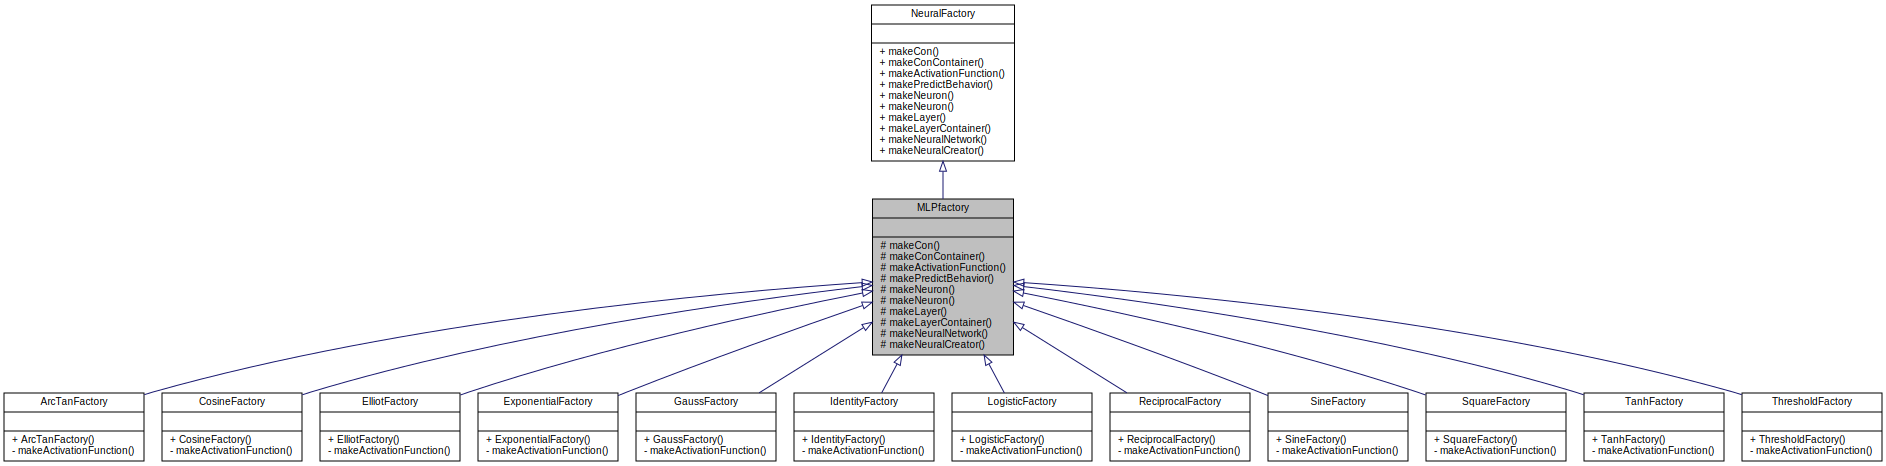
\includegraphics[width=400pt]{class_m_l_pfactory__inherit__graph}
\end{center}
\end{figure}


Collaboration diagram for MLPfactory:
\nopagebreak
\begin{figure}[H]
\begin{center}
\leavevmode
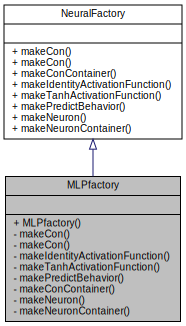
\includegraphics[width=222pt]{class_m_l_pfactory__coll__graph}
\end{center}
\end{figure}
\subsection*{Protected Member Functions}
\begin{DoxyCompactItemize}
\item 
\hyperlink{_a_m_o_r_e_8h_a169bb8e5f26ce70bf2b10dec2fb5ee50}{ConPtr} \hyperlink{class_m_l_pfactory_ac47beb4aced10b9c99414ba7dd7c8b55}{makeCon} (\hyperlink{class_neuron}{Neuron} \&neuron, double weight)
\item 
\hyperlink{_a_m_o_r_e_8h_a1021dbaf961d1c8da6d58a8566e5778b}{ConContainerPtr} \hyperlink{class_m_l_pfactory_a69562b8fd06c60a2d5db66d8b0f10299}{makeConContainer} ()
\item 
virtual \hyperlink{_a_m_o_r_e_8h_a77602a0277a02e5769c3df0adc669b17}{ActivationFunctionPtr} \hyperlink{class_m_l_pfactory_a92109ea285be7dd847d359a1ade9064a}{makeActivationFunction} (\hyperlink{_a_m_o_r_e_8h_ac1ea936c2c7728eb382278131652fef4}{NeuronPtr} neuronPtr)=0
\item 
\hyperlink{_a_m_o_r_e_8h_a1fb2f1f8fdf1e08c42ef4bdce436af93}{PredictBehaviorPtr} \hyperlink{class_m_l_pfactory_a9e9e9bb4390df09c78a24c4ff79cdab6}{makePredictBehavior} (\hyperlink{_a_m_o_r_e_8h_ac1ea936c2c7728eb382278131652fef4}{NeuronPtr} neuronPtr)
\item 
\hyperlink{_a_m_o_r_e_8h_ac1ea936c2c7728eb382278131652fef4}{NeuronPtr} \hyperlink{class_m_l_pfactory_a6dd50bc994fa69d7c4de183284efdae2}{makeNeuron} (\hyperlink{_a_m_o_r_e_8h_abc871abb71cff6655b8172ee7240b8ef}{Handler} Id)
\item 
\hyperlink{_a_m_o_r_e_8h_ac1ea936c2c7728eb382278131652fef4}{NeuronPtr} \hyperlink{class_m_l_pfactory_a9e3c7140a702a12d7a7fde8ad52b6b04}{makeNeuron} (\hyperlink{_a_m_o_r_e_8h_abc871abb71cff6655b8172ee7240b8ef}{Handler} Id, \hyperlink{_a_m_o_r_e_8h_aa794539c0a68e4eb451e7a2cc6294acc}{NeuronIteratorPtr} neuronIteratorPtr, double totalAmountOfParameters)
\item 
\hyperlink{_a_m_o_r_e_8h_acce4b66db3921b7326fbe1a04a56e5fc}{LayerPtr} \hyperlink{class_m_l_pfactory_ab67ef662094f7c74079d7d1af3d0a3ce}{makeLayer} ()
\item 
\hyperlink{_a_m_o_r_e_8h_af261b546158af61fc27686fb926961f2}{LayerContainerPtr} \hyperlink{class_m_l_pfactory_af12cd036035e6887869f22f4c5ecb497}{makeLayerContainer} ()
\item 
\hyperlink{_a_m_o_r_e_8h_a7adadf1c313313507b00cd1193db29a1}{NeuralNetworkPtr} \hyperlink{class_m_l_pfactory_abbedf3582eef72da1fdae1fd0a07a441}{makeNeuralNetwork} (\hyperlink{class_neural_factory}{NeuralFactory} \&neuralFactory)
\item 
\hyperlink{_a_m_o_r_e_8h_aefebabe3353f684b7708712480c15699}{NeuralCreatorPtr} \hyperlink{class_m_l_pfactory_ab71df59a90f1f32abdd52ff8b3f6fe7a}{makeNeuralCreator} ()
\end{DoxyCompactItemize}


\subsection{Detailed Description}
class \hyperlink{class_m_l_pfactory}{MLPfactory} -\/ 

Definition at line 5 of file MLPfactory.h.



\subsection{Member Function Documentation}
\hypertarget{class_m_l_pfactory_a92109ea285be7dd847d359a1ade9064a}{
\index{MLPfactory@{MLPfactory}!makeActivationFunction@{makeActivationFunction}}
\index{makeActivationFunction@{makeActivationFunction}!MLPfactory@{MLPfactory}}
\subsubsection[{makeActivationFunction}]{\setlength{\rightskip}{0pt plus 5cm}virtual {\bf ActivationFunctionPtr} MLPfactory::makeActivationFunction (
\begin{DoxyParamCaption}
\item[{{\bf NeuronPtr}}]{neuronPtr}
\end{DoxyParamCaption}
)\hspace{0.3cm}{\ttfamily  \mbox{[}protected, pure virtual\mbox{]}}}}
\label{class_m_l_pfactory_a92109ea285be7dd847d359a1ade9064a}


Implements \hyperlink{class_neural_factory_a678ec16456e5772a2c188c475a78c588}{NeuralFactory}.



Implemented in \hyperlink{class_arc_tan_factory_ae07c1b383c55ee42732d97fb2215d7fb}{ArcTanFactory}, \hyperlink{class_cosine_factory_a7db770cbd419032850a7e4f09b0836cc}{CosineFactory}, \hyperlink{class_elliot_factory_aedc7054f162dea077b2de6beaa7d1577}{ElliotFactory}, \hyperlink{class_exponential_factory_a68819f57ee476e87a2aa23827fc52578}{ExponentialFactory}, \hyperlink{class_gauss_factory_a0a937a783740366b0c07264f1d707ea7}{GaussFactory}, \hyperlink{class_identity_factory_a13a9bb3996539b46c4d9eee7c2024ea1}{IdentityFactory}, \hyperlink{class_logistic_factory_a43d3c7497e5f4058f514f86cfd25d9f8}{LogisticFactory}, \hyperlink{class_reciprocal_factory_a4258da65a19ff656c79bac5f2699b8d8}{ReciprocalFactory}, \hyperlink{class_sine_factory_aca81bca10dbcac538f58209270ebd26d}{SineFactory}, \hyperlink{class_square_factory_a1fe378c014b3713865f88c49e96ba938}{SquareFactory}, \hyperlink{class_tanh_factory_a476450ea27b571e3548377afd1625372}{TanhFactory}, and \hyperlink{class_threshold_factory_a6be00aaf355c02f73e1f818d3de8c548}{ThresholdFactory}.



Referenced by makeNeuron().



Here is the caller graph for this function:
\nopagebreak
\begin{figure}[H]
\begin{center}
\leavevmode
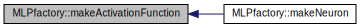
\includegraphics[width=400pt]{class_m_l_pfactory_a92109ea285be7dd847d359a1ade9064a_icgraph}
\end{center}
\end{figure}


\hypertarget{class_m_l_pfactory_ac47beb4aced10b9c99414ba7dd7c8b55}{
\index{MLPfactory@{MLPfactory}!makeCon@{makeCon}}
\index{makeCon@{makeCon}!MLPfactory@{MLPfactory}}
\subsubsection[{makeCon}]{\setlength{\rightskip}{0pt plus 5cm}{\bf ConPtr} MLPfactory::makeCon (
\begin{DoxyParamCaption}
\item[{{\bf Neuron} \&}]{neuron, }
\item[{double}]{weight}
\end{DoxyParamCaption}
)\hspace{0.3cm}{\ttfamily  \mbox{[}protected, virtual\mbox{]}}}}
\label{class_m_l_pfactory_ac47beb4aced10b9c99414ba7dd7c8b55}


Implements \hyperlink{class_neural_factory_a0d11171bb9e5d09544e8d58a9324b923}{NeuralFactory}.



Definition at line 30 of file MLPfactory.cpp.



Referenced by makeNeuron().


\begin{DoxyCode}
{
  ConPtr conPtr(new Con(neuron, weight));
  return conPtr;
}
\end{DoxyCode}


Here is the caller graph for this function:
\nopagebreak
\begin{figure}[H]
\begin{center}
\leavevmode
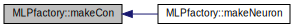
\includegraphics[width=366pt]{class_m_l_pfactory_ac47beb4aced10b9c99414ba7dd7c8b55_icgraph}
\end{center}
\end{figure}


\hypertarget{class_m_l_pfactory_a69562b8fd06c60a2d5db66d8b0f10299}{
\index{MLPfactory@{MLPfactory}!makeConContainer@{makeConContainer}}
\index{makeConContainer@{makeConContainer}!MLPfactory@{MLPfactory}}
\subsubsection[{makeConContainer}]{\setlength{\rightskip}{0pt plus 5cm}{\bf ConContainerPtr} MLPfactory::makeConContainer (
\begin{DoxyParamCaption}
{}
\end{DoxyParamCaption}
)\hspace{0.3cm}{\ttfamily  \mbox{[}protected, virtual\mbox{]}}}}
\label{class_m_l_pfactory_a69562b8fd06c60a2d5db66d8b0f10299}


Implements \hyperlink{class_neural_factory_a4fa5f4f57a2551c95481146b1a0c83d7}{NeuralFactory}.



Definition at line 37 of file MLPfactory.cpp.


\begin{DoxyCode}
{
  ConContainerPtr conContainerPtr(new SimpleContainer<ConPtr> );
  return conContainerPtr;
}
\end{DoxyCode}
\hypertarget{class_m_l_pfactory_ab67ef662094f7c74079d7d1af3d0a3ce}{
\index{MLPfactory@{MLPfactory}!makeLayer@{makeLayer}}
\index{makeLayer@{makeLayer}!MLPfactory@{MLPfactory}}
\subsubsection[{makeLayer}]{\setlength{\rightskip}{0pt plus 5cm}{\bf LayerPtr} MLPfactory::makeLayer (
\begin{DoxyParamCaption}
{}
\end{DoxyParamCaption}
)\hspace{0.3cm}{\ttfamily  \mbox{[}protected, virtual\mbox{]}}}}
\label{class_m_l_pfactory_ab67ef662094f7c74079d7d1af3d0a3ce}


Implements \hyperlink{class_neural_factory_a1a02bc2427430c4085654a72a03a5f4f}{NeuralFactory}.



Definition at line 84 of file MLPfactory.cpp.



Referenced by makeLayerContainer().


\begin{DoxyCode}
{
  LayerPtr layerPtr( new SimpleContainer<NeuronPtr> );
  return layerPtr;
}
\end{DoxyCode}


Here is the caller graph for this function:
\nopagebreak
\begin{figure}[H]
\begin{center}
\leavevmode
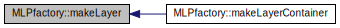
\includegraphics[width=400pt]{class_m_l_pfactory_ab67ef662094f7c74079d7d1af3d0a3ce_icgraph}
\end{center}
\end{figure}


\hypertarget{class_m_l_pfactory_af12cd036035e6887869f22f4c5ecb497}{
\index{MLPfactory@{MLPfactory}!makeLayerContainer@{makeLayerContainer}}
\index{makeLayerContainer@{makeLayerContainer}!MLPfactory@{MLPfactory}}
\subsubsection[{makeLayerContainer}]{\setlength{\rightskip}{0pt plus 5cm}{\bf LayerContainerPtr} MLPfactory::makeLayerContainer (
\begin{DoxyParamCaption}
{}
\end{DoxyParamCaption}
)\hspace{0.3cm}{\ttfamily  \mbox{[}protected, virtual\mbox{]}}}}
\label{class_m_l_pfactory_af12cd036035e6887869f22f4c5ecb497}


Implements \hyperlink{class_neural_factory_a10b5056a57cc3fef56c66da1ad367fc7}{NeuralFactory}.



Definition at line 92 of file MLPfactory.cpp.



References makeLayer().


\begin{DoxyCode}
{
  LayerContainerPtr layerContainerPtr( new SimpleContainer<LayerPtr> );
  layerContainerPtr->push_back( makeLayer() );
  return layerContainerPtr;
}
\end{DoxyCode}


Here is the call graph for this function:
\nopagebreak
\begin{figure}[H]
\begin{center}
\leavevmode
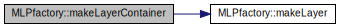
\includegraphics[width=400pt]{class_m_l_pfactory_af12cd036035e6887869f22f4c5ecb497_cgraph}
\end{center}
\end{figure}


\hypertarget{class_m_l_pfactory_ab71df59a90f1f32abdd52ff8b3f6fe7a}{
\index{MLPfactory@{MLPfactory}!makeNeuralCreator@{makeNeuralCreator}}
\index{makeNeuralCreator@{makeNeuralCreator}!MLPfactory@{MLPfactory}}
\subsubsection[{makeNeuralCreator}]{\setlength{\rightskip}{0pt plus 5cm}{\bf NeuralCreatorPtr} MLPfactory::makeNeuralCreator (
\begin{DoxyParamCaption}
{}
\end{DoxyParamCaption}
)\hspace{0.3cm}{\ttfamily  \mbox{[}protected, virtual\mbox{]}}}}
\label{class_m_l_pfactory_ab71df59a90f1f32abdd52ff8b3f6fe7a}


Implements \hyperlink{class_neural_factory_a2c7502e1bf81d3fc33284123d733428e}{NeuralFactory}.



Definition at line 109 of file MLPfactory.cpp.


\begin{DoxyCode}
{
  NeuralCreatorPtr neuralCreatorPtr(new SimpleNeuralCreator );
  return neuralCreatorPtr;
}
\end{DoxyCode}
\hypertarget{class_m_l_pfactory_abbedf3582eef72da1fdae1fd0a07a441}{
\index{MLPfactory@{MLPfactory}!makeNeuralNetwork@{makeNeuralNetwork}}
\index{makeNeuralNetwork@{makeNeuralNetwork}!MLPfactory@{MLPfactory}}
\subsubsection[{makeNeuralNetwork}]{\setlength{\rightskip}{0pt plus 5cm}{\bf NeuralNetworkPtr} MLPfactory::makeNeuralNetwork (
\begin{DoxyParamCaption}
\item[{{\bf NeuralFactory} \&}]{neuralFactory}
\end{DoxyParamCaption}
)\hspace{0.3cm}{\ttfamily  \mbox{[}protected, virtual\mbox{]}}}}
\label{class_m_l_pfactory_abbedf3582eef72da1fdae1fd0a07a441}


Implements \hyperlink{class_neural_factory_a15b9308e868ca439869b1d68afabfcde}{NeuralFactory}.



Definition at line 101 of file MLPfactory.cpp.


\begin{DoxyCode}
{
  NeuralNetworkPtr neuralNetworkPtr(new SimpleNetwork(neuralFactory ) );
  return neuralNetworkPtr;
}
\end{DoxyCode}
\hypertarget{class_m_l_pfactory_a6dd50bc994fa69d7c4de183284efdae2}{
\index{MLPfactory@{MLPfactory}!makeNeuron@{makeNeuron}}
\index{makeNeuron@{makeNeuron}!MLPfactory@{MLPfactory}}
\subsubsection[{makeNeuron}]{\setlength{\rightskip}{0pt plus 5cm}{\bf NeuronPtr} MLPfactory::makeNeuron (
\begin{DoxyParamCaption}
\item[{{\bf Handler}}]{Id}
\end{DoxyParamCaption}
)\hspace{0.3cm}{\ttfamily  \mbox{[}protected, virtual\mbox{]}}}}
\label{class_m_l_pfactory_a6dd50bc994fa69d7c4de183284efdae2}


Implements \hyperlink{class_neural_factory_a12abbf93f829aab585975f157c8c98f7}{NeuralFactory}.



Definition at line 52 of file MLPfactory.cpp.



References makeActivationFunction(), and makePredictBehavior().



Referenced by makeNeuron().


\begin{DoxyCode}
{
  NeuronPtr neuronPtr(new SimpleNeuron(*this));
  neuronPtr->setId(Id);
  neuronPtr->setPredictBehavior(makePredictBehavior(neuronPtr));
  neuronPtr->setActivationFunction(makeActivationFunction(neuronPtr));
  return neuronPtr;
}
\end{DoxyCode}


Here is the call graph for this function:
\nopagebreak
\begin{figure}[H]
\begin{center}
\leavevmode
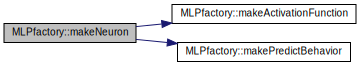
\includegraphics[width=400pt]{class_m_l_pfactory_a6dd50bc994fa69d7c4de183284efdae2_cgraph}
\end{center}
\end{figure}




Here is the caller graph for this function:
\nopagebreak
\begin{figure}[H]
\begin{center}
\leavevmode
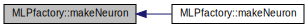
\includegraphics[width=380pt]{class_m_l_pfactory_a6dd50bc994fa69d7c4de183284efdae2_icgraph}
\end{center}
\end{figure}


\hypertarget{class_m_l_pfactory_a9e3c7140a702a12d7a7fde8ad52b6b04}{
\index{MLPfactory@{MLPfactory}!makeNeuron@{makeNeuron}}
\index{makeNeuron@{makeNeuron}!MLPfactory@{MLPfactory}}
\subsubsection[{makeNeuron}]{\setlength{\rightskip}{0pt plus 5cm}{\bf NeuronPtr} MLPfactory::makeNeuron (
\begin{DoxyParamCaption}
\item[{{\bf Handler}}]{Id, }
\item[{{\bf NeuronIteratorPtr}}]{neuronIteratorPtr, }
\item[{double}]{totalAmountOfParameters}
\end{DoxyParamCaption}
)\hspace{0.3cm}{\ttfamily  \mbox{[}protected, virtual\mbox{]}}}}
\label{class_m_l_pfactory_a9e3c7140a702a12d7a7fde8ad52b6b04}


Implements \hyperlink{class_neural_factory_a19c08ba7ad05ef7af05f7595dda2100b}{NeuralFactory}.



Definition at line 62 of file MLPfactory.cpp.



References MLPbehavior::d\_\-bias, makeCon(), and makeNeuron().


\begin{DoxyCode}
{
  RNGScope scope;

  NeuronPtr neuronPtr(makeNeuron(Id));

  double extreme = sqrt(3 / totalAmountOfParameters);
  double weight;
  for (neuronIteratorPtr->first(); !neuronIteratorPtr->isDone(); neuronIteratorPt
      r->next())
    {
      weight =as<double>(runif(1, -extreme, extreme));
      neuronPtr->addCon(makeCon(*neuronIteratorPtr->currentItem(), weight));
    }

  MLPbehavior* mlpBehavior = dynamic_cast<MLPbehavior*>(neuronPtr->d_predictBehav
      ior.get()) ;
  mlpBehavior->d_bias=as<double>(runif(1, -extreme, extreme));

return neuronPtr;
}
\end{DoxyCode}


Here is the call graph for this function:
\nopagebreak
\begin{figure}[H]
\begin{center}
\leavevmode
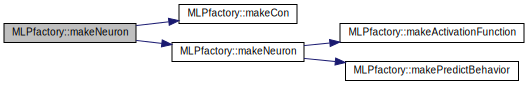
\includegraphics[width=400pt]{class_m_l_pfactory_a9e3c7140a702a12d7a7fde8ad52b6b04_cgraph}
\end{center}
\end{figure}


\hypertarget{class_m_l_pfactory_a9e9e9bb4390df09c78a24c4ff79cdab6}{
\index{MLPfactory@{MLPfactory}!makePredictBehavior@{makePredictBehavior}}
\index{makePredictBehavior@{makePredictBehavior}!MLPfactory@{MLPfactory}}
\subsubsection[{makePredictBehavior}]{\setlength{\rightskip}{0pt plus 5cm}{\bf PredictBehaviorPtr} MLPfactory::makePredictBehavior (
\begin{DoxyParamCaption}
\item[{{\bf NeuronPtr}}]{neuronPtr}
\end{DoxyParamCaption}
)\hspace{0.3cm}{\ttfamily  \mbox{[}protected, virtual\mbox{]}}}}
\label{class_m_l_pfactory_a9e9e9bb4390df09c78a24c4ff79cdab6}


Implements \hyperlink{class_neural_factory_a3d49ef5f05c82cc2c614e884ed3a27d5}{NeuralFactory}.



Definition at line 45 of file MLPfactory.cpp.



Referenced by makeNeuron().


\begin{DoxyCode}
{
  PredictBehaviorPtr predictBehaviorPtr(new MLPbehavior(neuronPtr));
  return predictBehaviorPtr;
}
\end{DoxyCode}


Here is the caller graph for this function:
\nopagebreak
\begin{figure}[H]
\begin{center}
\leavevmode
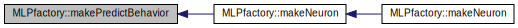
\includegraphics[width=400pt]{class_m_l_pfactory_a9e9e9bb4390df09c78a24c4ff79cdab6_icgraph}
\end{center}
\end{figure}




The documentation for this class was generated from the following files:\begin{DoxyCompactItemize}
\item 
/Users/mcasl/pc-\/ule/Trabajo/investigacion/AMORE/AMORE-\/WC/AMORE-\/WC/pkg/AMORE/src/classHeaders/\hyperlink{_m_l_pfactory_8h}{MLPfactory.h}\item 
/Users/mcasl/pc-\/ule/Trabajo/investigacion/AMORE/AMORE-\/WC/AMORE-\/WC/pkg/AMORE/src/\hyperlink{_m_l_pfactory_8cpp}{MLPfactory.cpp}\end{DoxyCompactItemize}

\hypertarget{class_neural_creator}{
\section{NeuralCreator Class Reference}
\label{class_neural_creator}\index{NeuralCreator@{NeuralCreator}}
}


class \hyperlink{class_neural_creator}{NeuralCreator} -\/  




{\ttfamily \#include $<$NeuralCreator.h$>$}



Inheritance diagram for NeuralCreator:
\nopagebreak
\begin{figure}[H]
\begin{center}
\leavevmode
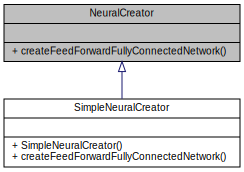
\includegraphics[width=210pt]{class_neural_creator__inherit__graph}
\end{center}
\end{figure}
\subsection*{Public Member Functions}
\begin{DoxyCompactItemize}
\item 
virtual \hyperlink{_a_m_o_r_e_8h_ac1ea936c2c7728eb382278131652fef4}{NeuronPtr} \hyperlink{class_neural_creator_abfff3986cb184e493107692eab3dc678}{createNeuron} (\hyperlink{_a_m_o_r_e_8h_ac4ad88962955479bfc426da9ce4571d2}{NeuralFactoryPtr} neuralFactoryPtr)=0
\end{DoxyCompactItemize}


\subsection{Detailed Description}
class \hyperlink{class_neural_creator}{NeuralCreator} -\/ 

Definition at line 4 of file NeuralCreator.h.



\subsection{Member Function Documentation}
\hypertarget{class_neural_creator_abfff3986cb184e493107692eab3dc678}{
\index{NeuralCreator@{NeuralCreator}!createNeuron@{createNeuron}}
\index{createNeuron@{createNeuron}!NeuralCreator@{NeuralCreator}}
\subsubsection[{createNeuron}]{\setlength{\rightskip}{0pt plus 5cm}virtual {\bf NeuronPtr} NeuralCreator::createNeuron (
\begin{DoxyParamCaption}
\item[{{\bf NeuralFactoryPtr}}]{neuralFactoryPtr}
\end{DoxyParamCaption}
)\hspace{0.3cm}{\ttfamily  \mbox{[}pure virtual\mbox{]}}}}
\label{class_neural_creator_abfff3986cb184e493107692eab3dc678}


Implemented in \hyperlink{class_simple_neural_creator_a9644ba2572c29a119d54c071611a52b2}{SimpleNeuralCreator}.



The documentation for this class was generated from the following file:\begin{DoxyCompactItemize}
\item 
pkg/AMORE/src/dia/\hyperlink{_neural_creator_8h}{NeuralCreator.h}\end{DoxyCompactItemize}

\hypertarget{class_neural_factory}{
\section{NeuralFactory Class Reference}
\label{class_neural_factory}\index{NeuralFactory@{NeuralFactory}}
}


class \hyperlink{class_neural_factory}{NeuralFactory} -\/  




{\ttfamily \#include $<$NeuralFactory.h$>$}



Inheritance diagram for NeuralFactory:\nopagebreak
\begin{figure}[H]
\begin{center}
\leavevmode
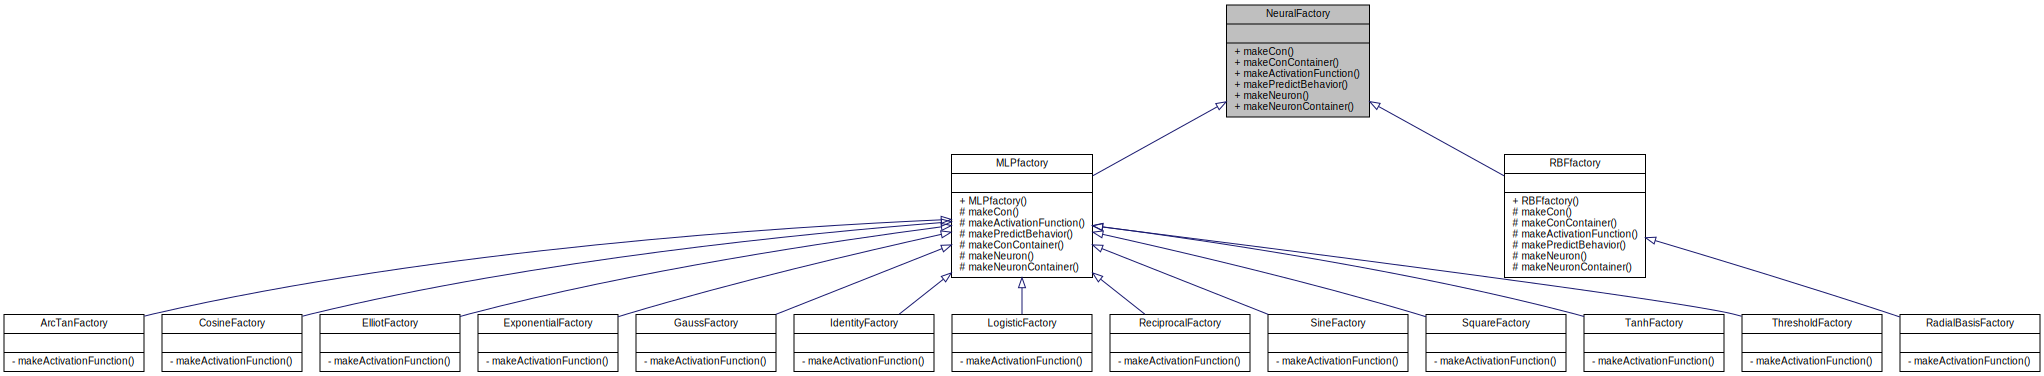
\includegraphics[width=362pt]{class_neural_factory__inherit__graph}
\end{center}
\end{figure}
\subsection*{Public Member Functions}
\begin{DoxyCompactItemize}
\item 
virtual \hyperlink{class_con}{Con} $\ast$ \hyperlink{class_neural_factory_ad7dacdd1ed0994f4a55612bd2d45ada2}{makeCon} (\hyperlink{class_neuron}{Neuron} \&neuron)=0
\item 
virtual \hyperlink{class_con}{Con} $\ast$ \hyperlink{class_neural_factory_a1f466a7f82020767cda89ae48a9852b7}{makeCon} (\hyperlink{class_neuron}{Neuron} \&neuron, double weight)=0
\item 
virtual \hyperlink{class_container}{Container}$<$ \hyperlink{_a_m_o_r_e_8h_a169bb8e5f26ce70bf2b10dec2fb5ee50}{ConPtr} $>$ $\ast$ \hyperlink{class_neural_factory_a0446aa979904fc0c5f6cda9bf1044100}{makeConContainer} ()=0
\item 
virtual \hyperlink{class_container}{Container}$<$ \hyperlink{_a_m_o_r_e_8h_ac1ea936c2c7728eb382278131652fef4}{NeuronPtr} $>$ $\ast$ \hyperlink{class_neural_factory_a1f56d9485fe3669a79d5d5dc70be65af}{makeNeuronContainer} ()=0
\item 
virtual \hyperlink{class_neuron}{Neuron} $\ast$ \hyperlink{class_neural_factory_a656b7663182769bcfd5ce5940e03b7cd}{makeNeuron} ()=0
\end{DoxyCompactItemize}


\subsection{Detailed Description}
class \hyperlink{class_neural_factory}{NeuralFactory} -\/ 

Definition at line 4 of file NeuralFactory.h.



\subsection{Member Function Documentation}
\hypertarget{class_neural_factory_ad7dacdd1ed0994f4a55612bd2d45ada2}{
\index{NeuralFactory@{NeuralFactory}!makeCon@{makeCon}}
\index{makeCon@{makeCon}!NeuralFactory@{NeuralFactory}}
\subsubsection[{makeCon}]{\setlength{\rightskip}{0pt plus 5cm}virtual {\bf Con}$\ast$ NeuralFactory::makeCon (
\begin{DoxyParamCaption}
\item[{{\bf Neuron} \&}]{neuron}
\end{DoxyParamCaption}
)\hspace{0.3cm}{\ttfamily  \mbox{[}pure virtual\mbox{]}}}}
\label{class_neural_factory_ad7dacdd1ed0994f4a55612bd2d45ada2}


Implemented in \hyperlink{class_m_l_pfactory_a479b674ed4e63bb1178c091325c2cd61}{MLPfactory}, and \hyperlink{class_r_b_ffactory_a0cb9bbdd1726e28de699eceba731808b}{RBFfactory}.



Referenced by SimpleNeuralCreator::createCon().



Here is the caller graph for this function:\nopagebreak
\begin{figure}[H]
\begin{center}
\leavevmode
\includegraphics[width=400pt]{class_neural_factory_ad7dacdd1ed0994f4a55612bd2d45ada2_icgraph}
\end{center}
\end{figure}


\hypertarget{class_neural_factory_a1f466a7f82020767cda89ae48a9852b7}{
\index{NeuralFactory@{NeuralFactory}!makeCon@{makeCon}}
\index{makeCon@{makeCon}!NeuralFactory@{NeuralFactory}}
\subsubsection[{makeCon}]{\setlength{\rightskip}{0pt plus 5cm}virtual {\bf Con}$\ast$ NeuralFactory::makeCon (
\begin{DoxyParamCaption}
\item[{{\bf Neuron} \&}]{neuron, }
\item[{double}]{weight}
\end{DoxyParamCaption}
)\hspace{0.3cm}{\ttfamily  \mbox{[}pure virtual\mbox{]}}}}
\label{class_neural_factory_a1f466a7f82020767cda89ae48a9852b7}


Implemented in \hyperlink{class_m_l_pfactory_a18c3770c3cb2ed6c3cb402cb814b209c}{MLPfactory}.

\hypertarget{class_neural_factory_a0446aa979904fc0c5f6cda9bf1044100}{
\index{NeuralFactory@{NeuralFactory}!makeConContainer@{makeConContainer}}
\index{makeConContainer@{makeConContainer}!NeuralFactory@{NeuralFactory}}
\subsubsection[{makeConContainer}]{\setlength{\rightskip}{0pt plus 5cm}virtual {\bf Container}$<${\bf ConPtr}$>$$\ast$ NeuralFactory::makeConContainer (
\begin{DoxyParamCaption}
{}
\end{DoxyParamCaption}
)\hspace{0.3cm}{\ttfamily  \mbox{[}pure virtual\mbox{]}}}}
\label{class_neural_factory_a0446aa979904fc0c5f6cda9bf1044100}


Implemented in \hyperlink{class_m_l_pfactory_a62ea35a5b7ce5f139f91b2c3edd4ad61}{MLPfactory}, and \hyperlink{class_r_b_ffactory_a844c8fdc315958fdb084194f0b900c68}{RBFfactory}.

\hypertarget{class_neural_factory_a656b7663182769bcfd5ce5940e03b7cd}{
\index{NeuralFactory@{NeuralFactory}!makeNeuron@{makeNeuron}}
\index{makeNeuron@{makeNeuron}!NeuralFactory@{NeuralFactory}}
\subsubsection[{makeNeuron}]{\setlength{\rightskip}{0pt plus 5cm}virtual {\bf Neuron}$\ast$ NeuralFactory::makeNeuron (
\begin{DoxyParamCaption}
{}
\end{DoxyParamCaption}
)\hspace{0.3cm}{\ttfamily  \mbox{[}pure virtual\mbox{]}}}}
\label{class_neural_factory_a656b7663182769bcfd5ce5940e03b7cd}


Implemented in \hyperlink{class_m_l_pfactory_ac39058170421f03dfd88c2ced318f46b}{MLPfactory}, and \hyperlink{class_r_b_ffactory_aa3514a25f378fa5e677970018d2ce65e}{RBFfactory}.



Referenced by SimpleNeuralCreator::createNeuron().



Here is the caller graph for this function:\nopagebreak
\begin{figure}[H]
\begin{center}
\leavevmode
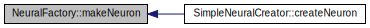
\includegraphics[width=400pt]{class_neural_factory_a656b7663182769bcfd5ce5940e03b7cd_icgraph}
\end{center}
\end{figure}


\hypertarget{class_neural_factory_a1f56d9485fe3669a79d5d5dc70be65af}{
\index{NeuralFactory@{NeuralFactory}!makeNeuronContainer@{makeNeuronContainer}}
\index{makeNeuronContainer@{makeNeuronContainer}!NeuralFactory@{NeuralFactory}}
\subsubsection[{makeNeuronContainer}]{\setlength{\rightskip}{0pt plus 5cm}virtual {\bf Container}$<${\bf NeuronPtr}$>$$\ast$ NeuralFactory::makeNeuronContainer (
\begin{DoxyParamCaption}
{}
\end{DoxyParamCaption}
)\hspace{0.3cm}{\ttfamily  \mbox{[}pure virtual\mbox{]}}}}
\label{class_neural_factory_a1f56d9485fe3669a79d5d5dc70be65af}


Implemented in \hyperlink{class_m_l_pfactory_a18bbb914f7b974c0f8c5dd3913f6dd1c}{MLPfactory}, and \hyperlink{class_r_b_ffactory_a92fc16863bf60ebd93be1f108ce95ad6}{RBFfactory}.



The documentation for this class was generated from the following file:\begin{DoxyCompactItemize}
\item 
pkg/AMORE/src/dia/\hyperlink{_neural_factory_8h}{NeuralFactory.h}\end{DoxyCompactItemize}

\hypertarget{class_neuron}{
\section{Neuron Class Reference}
\label{class_neuron}\index{Neuron@{Neuron}}
}


A class to handle the information contained in a general \hyperlink{class_neuron}{Neuron}.  




{\ttfamily \#include $<$Neuron.h$>$}



Collaboration diagram for Neuron:
\nopagebreak
\begin{figure}[H]
\begin{center}
\leavevmode
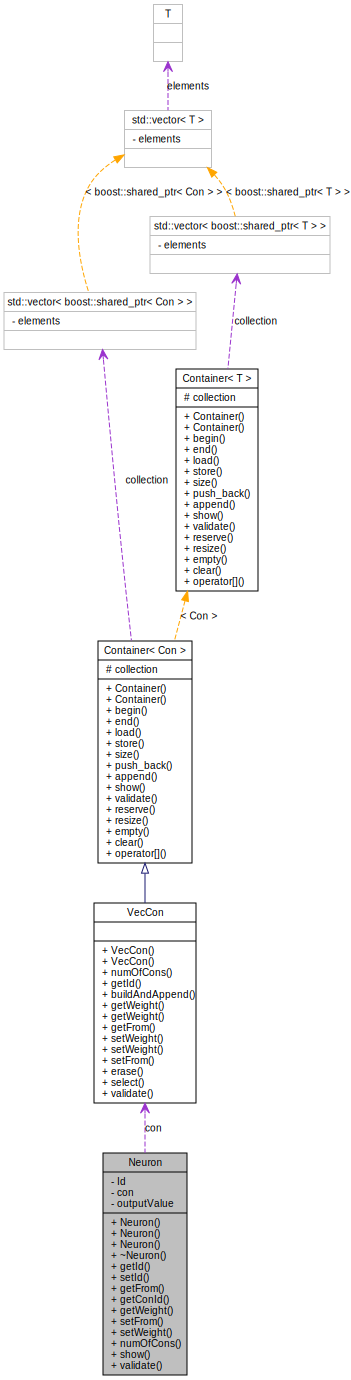
\includegraphics[height=600pt]{class_neuron__coll__graph}
\end{center}
\end{figure}
\subsection*{Public Member Functions}
\begin{DoxyCompactItemize}
\item 
\hyperlink{class_neuron_a823487d01615fadb8ac19a2768dd9d96}{Neuron} ()
\item 
\hyperlink{class_neuron_a05698a11ac18b6cee34d18f63681ddcc}{Neuron} (int \hyperlink{class_neuron_a72bb327a7c5c865e6748a4e074ce0680}{Id})
\item 
\hyperlink{class_neuron_af6ba81347cc25d4d5d256dba2c4e441a}{Neuron} (int \hyperlink{class_neuron_a72bb327a7c5c865e6748a4e074ce0680}{Id}, \hyperlink{class_vec_con}{VecCon} \hyperlink{class_con}{Con})
\item 
\hyperlink{class_neuron_a94a250ce7e167760e593979b899745b1}{$\sim$Neuron} ()
\item 
int \hyperlink{class_neuron_ad9211d55ea50ad6dfbd2676b9e2335e4}{getId} ()
\item 
void \hyperlink{class_neuron_a6eb17a0d297b8c65170911aff37ba968}{setId} (int \hyperlink{class_neuron_a72bb327a7c5c865e6748a4e074ce0680}{Id})
\item 
std::vector$<$ \hyperlink{_a_m_o_r_e_8h_ac1ea936c2c7728eb382278131652fef4}{NeuronPtr} $>$ \hyperlink{class_neuron_a66e3800037d2789a8fe7b73996c14f84}{getFrom} ()
\item 
std::vector$<$ int $>$ \hyperlink{class_neuron_aac7d538b4a5087f730ba80f19852bced}{getConId} ()
\item 
std::vector$<$ double $>$ \hyperlink{class_neuron_a3349c0a2053e35afa5b7036bb816f8c6}{getWeight} ()
\item 
bool \hyperlink{class_neuron_ace0e92348f8a5604f25a3cfc07f38ec8}{setFrom} (std::vector$<$ \hyperlink{_a_m_o_r_e_8h_ac1ea936c2c7728eb382278131652fef4}{NeuronPtr} $>$ vFrom)
\item 
bool \hyperlink{class_neuron_ab067bfe507f5386eccc860d4ad2d0bca}{setWeight} (std::vector$<$ double $>$ vWeight)
\item 
int \hyperlink{class_neuron_ae447dce39ed04581609a83d742b585d1}{numOfCons} ()
\item 
bool \hyperlink{class_neuron_a255c3597520c730d798218f7174eff1b}{show} ()
\item 
bool \hyperlink{class_neuron_a95327aa80a9ec949491f214a0c159b5a}{validate} ()
\end{DoxyCompactItemize}
\subsection*{Private Attributes}
\begin{DoxyCompactItemize}
\item 
int \hyperlink{class_neuron_a72bb327a7c5c865e6748a4e074ce0680}{Id}
\begin{DoxyCompactList}\small\item\em An integer variable with the \hyperlink{class_neuron}{Neuron} Id. \end{DoxyCompactList}\item 
\hyperlink{class_vec_con}{VecCon} \hyperlink{class_neuron_a1451f2424a8f9e46ca643d03ff98a616}{con}
\begin{DoxyCompactList}\small\item\em A vector of input connections. \end{DoxyCompactList}\item 
double \hyperlink{class_neuron_ada029047646c36e525a6a1b77cafc03c}{outputValue}
\end{DoxyCompactItemize}


\subsection{Detailed Description}
A class to handle the information contained in a general \hyperlink{class_neuron}{Neuron}. 

A general class for neurons. The MLPneuron and RBFneuron classes will specialize this general class 

Definition at line 16 of file Neuron.h.



\subsection{Constructor \& Destructor Documentation}
\hypertarget{class_neuron_a823487d01615fadb8ac19a2768dd9d96}{
\index{Neuron@{Neuron}!Neuron@{Neuron}}
\index{Neuron@{Neuron}!Neuron@{Neuron}}
\subsubsection[{Neuron}]{\setlength{\rightskip}{0pt plus 5cm}Neuron::Neuron (
\begin{DoxyParamCaption}
{}
\end{DoxyParamCaption}
)}}
\label{class_neuron_a823487d01615fadb8ac19a2768dd9d96}


Definition at line 12 of file Neuron.cpp.


\begin{DoxyCode}
: Id(NA_INTEGER), con() {};
\end{DoxyCode}
\hypertarget{class_neuron_a05698a11ac18b6cee34d18f63681ddcc}{
\index{Neuron@{Neuron}!Neuron@{Neuron}}
\index{Neuron@{Neuron}!Neuron@{Neuron}}
\subsubsection[{Neuron}]{\setlength{\rightskip}{0pt plus 5cm}Neuron::Neuron (
\begin{DoxyParamCaption}
\item[{int}]{Id}
\end{DoxyParamCaption}
)}}
\label{class_neuron_a05698a11ac18b6cee34d18f63681ddcc}


Definition at line 13 of file Neuron.cpp.


\begin{DoxyCode}
: Id(Id), outputValue(0.0) {};
\end{DoxyCode}
\hypertarget{class_neuron_af6ba81347cc25d4d5d256dba2c4e441a}{
\index{Neuron@{Neuron}!Neuron@{Neuron}}
\index{Neuron@{Neuron}!Neuron@{Neuron}}
\subsubsection[{Neuron}]{\setlength{\rightskip}{0pt plus 5cm}Neuron::Neuron (
\begin{DoxyParamCaption}
\item[{int}]{Id, }
\item[{{\bf VecCon}}]{Con}
\end{DoxyParamCaption}
)}}
\label{class_neuron_af6ba81347cc25d4d5d256dba2c4e441a}


Definition at line 14 of file Neuron.cpp.


\begin{DoxyCode}
: Id(Id), con(con), outputValue(0.0) {} ;
\end{DoxyCode}
\hypertarget{class_neuron_a94a250ce7e167760e593979b899745b1}{
\index{Neuron@{Neuron}!$\sim$Neuron@{$\sim$Neuron}}
\index{$\sim$Neuron@{$\sim$Neuron}!Neuron@{Neuron}}
\subsubsection[{$\sim$Neuron}]{\setlength{\rightskip}{0pt plus 5cm}Neuron::$\sim$Neuron (
\begin{DoxyParamCaption}
{}
\end{DoxyParamCaption}
)}}
\label{class_neuron_a94a250ce7e167760e593979b899745b1}


Definition at line 15 of file Neuron.cpp.


\begin{DoxyCode}
{};
\end{DoxyCode}


\subsection{Member Function Documentation}
\hypertarget{class_neuron_aac7d538b4a5087f730ba80f19852bced}{
\index{Neuron@{Neuron}!getConId@{getConId}}
\index{getConId@{getConId}!Neuron@{Neuron}}
\subsubsection[{getConId}]{\setlength{\rightskip}{0pt plus 5cm}std::vector$<$ int $>$ Neuron::getConId (
\begin{DoxyParamCaption}
{}
\end{DoxyParamCaption}
)}}
\label{class_neuron_aac7d538b4a5087f730ba80f19852bced}


Definition at line 32 of file Neuron.cpp.



References con, and VecCon::getId().


\begin{DoxyCode}
                                  {
        return con.getId();
}
\end{DoxyCode}


Here is the call graph for this function:
\nopagebreak
\begin{figure}[H]
\begin{center}
\leavevmode
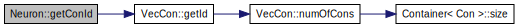
\includegraphics[width=400pt]{class_neuron_aac7d538b4a5087f730ba80f19852bced_cgraph}
\end{center}
\end{figure}


\hypertarget{class_neuron_a66e3800037d2789a8fe7b73996c14f84}{
\index{Neuron@{Neuron}!getFrom@{getFrom}}
\index{getFrom@{getFrom}!Neuron@{Neuron}}
\subsubsection[{getFrom}]{\setlength{\rightskip}{0pt plus 5cm}std::vector$<$ {\bf NeuronPtr} $>$ Neuron::getFrom (
\begin{DoxyParamCaption}
{}
\end{DoxyParamCaption}
)}}
\label{class_neuron_a66e3800037d2789a8fe7b73996c14f84}


Definition at line 27 of file Neuron.cpp.



References con, and VecCon::getFrom().


\begin{DoxyCode}
                                                  {
        return con.getFrom();
}
\end{DoxyCode}


Here is the call graph for this function:
\nopagebreak
\begin{figure}[H]
\begin{center}
\leavevmode
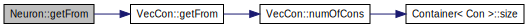
\includegraphics[width=400pt]{class_neuron_a66e3800037d2789a8fe7b73996c14f84_cgraph}
\end{center}
\end{figure}


\hypertarget{class_neuron_ad9211d55ea50ad6dfbd2676b9e2335e4}{
\index{Neuron@{Neuron}!getId@{getId}}
\index{getId@{getId}!Neuron@{Neuron}}
\subsubsection[{getId}]{\setlength{\rightskip}{0pt plus 5cm}int Neuron::getId (
\begin{DoxyParamCaption}
{}
\end{DoxyParamCaption}
)}}
\label{class_neuron_ad9211d55ea50ad6dfbd2676b9e2335e4}


Definition at line 18 of file Neuron.cpp.



References Id.



Referenced by show(), and validate().


\begin{DoxyCode}
                  {
        return Id;
}
\end{DoxyCode}


Here is the caller graph for this function:\nopagebreak
\begin{figure}[H]
\begin{center}
\leavevmode
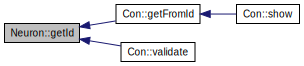
\includegraphics[width=280pt]{class_neuron_ad9211d55ea50ad6dfbd2676b9e2335e4_icgraph}
\end{center}
\end{figure}


\hypertarget{class_neuron_a3349c0a2053e35afa5b7036bb816f8c6}{
\index{Neuron@{Neuron}!getWeight@{getWeight}}
\index{getWeight@{getWeight}!Neuron@{Neuron}}
\subsubsection[{getWeight}]{\setlength{\rightskip}{0pt plus 5cm}std::vector$<$ double $>$ Neuron::getWeight (
\begin{DoxyParamCaption}
{}
\end{DoxyParamCaption}
)}}
\label{class_neuron_a3349c0a2053e35afa5b7036bb816f8c6}


Definition at line 37 of file Neuron.cpp.



References con, and VecCon::getWeight().


\begin{DoxyCode}
                                          {
        return con.getWeight();
}
\end{DoxyCode}


Here is the call graph for this function:
\nopagebreak
\begin{figure}[H]
\begin{center}
\leavevmode
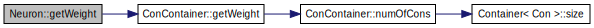
\includegraphics[width=400pt]{class_neuron_a3349c0a2053e35afa5b7036bb816f8c6_cgraph}
\end{center}
\end{figure}


\hypertarget{class_neuron_ae447dce39ed04581609a83d742b585d1}{
\index{Neuron@{Neuron}!numOfCons@{numOfCons}}
\index{numOfCons@{numOfCons}!Neuron@{Neuron}}
\subsubsection[{numOfCons}]{\setlength{\rightskip}{0pt plus 5cm}int Neuron::numOfCons (
\begin{DoxyParamCaption}
{}
\end{DoxyParamCaption}
)}}
\label{class_neuron_ae447dce39ed04581609a83d742b585d1}


Definition at line 51 of file Neuron.cpp.



References con, and VecCon::numOfCons().



Referenced by show().


\begin{DoxyCode}
                          {
        return con.numOfCons();
}
\end{DoxyCode}


Here is the call graph for this function:
\nopagebreak
\begin{figure}[H]
\begin{center}
\leavevmode
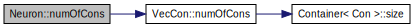
\includegraphics[width=400pt]{class_neuron_ae447dce39ed04581609a83d742b585d1_cgraph}
\end{center}
\end{figure}




Here is the caller graph for this function:
\nopagebreak
\begin{figure}[H]
\begin{center}
\leavevmode
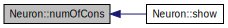
\includegraphics[width=300pt]{class_neuron_ae447dce39ed04581609a83d742b585d1_icgraph}
\end{center}
\end{figure}


\hypertarget{class_neuron_ace0e92348f8a5604f25a3cfc07f38ec8}{
\index{Neuron@{Neuron}!setFrom@{setFrom}}
\index{setFrom@{setFrom}!Neuron@{Neuron}}
\subsubsection[{setFrom}]{\setlength{\rightskip}{0pt plus 5cm}bool Neuron::setFrom (
\begin{DoxyParamCaption}
\item[{std::vector$<$ {\bf NeuronPtr} $>$}]{vFrom}
\end{DoxyParamCaption}
)}}
\label{class_neuron_ace0e92348f8a5604f25a3cfc07f38ec8}


Definition at line 42 of file Neuron.cpp.



References con, and VecCon::setFrom().


\begin{DoxyCode}
                                                            {
        con.setFrom(vFrom);
}
\end{DoxyCode}


Here is the call graph for this function:
\nopagebreak
\begin{figure}[H]
\begin{center}
\leavevmode
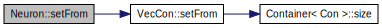
\includegraphics[width=400pt]{class_neuron_ace0e92348f8a5604f25a3cfc07f38ec8_cgraph}
\end{center}
\end{figure}


\hypertarget{class_neuron_a6eb17a0d297b8c65170911aff37ba968}{
\index{Neuron@{Neuron}!setId@{setId}}
\index{setId@{setId}!Neuron@{Neuron}}
\subsubsection[{setId}]{\setlength{\rightskip}{0pt plus 5cm}void Neuron::setId (
\begin{DoxyParamCaption}
\item[{int}]{Id}
\end{DoxyParamCaption}
)}}
\label{class_neuron_a6eb17a0d297b8c65170911aff37ba968}


Definition at line 22 of file Neuron.cpp.



References Id.


\begin{DoxyCode}
                         {
        Id=id;
}
\end{DoxyCode}
\hypertarget{class_neuron_ab067bfe507f5386eccc860d4ad2d0bca}{
\index{Neuron@{Neuron}!setWeight@{setWeight}}
\index{setWeight@{setWeight}!Neuron@{Neuron}}
\subsubsection[{setWeight}]{\setlength{\rightskip}{0pt plus 5cm}bool Neuron::setWeight (
\begin{DoxyParamCaption}
\item[{std::vector$<$ double $>$}]{vWeight}
\end{DoxyParamCaption}
)}}
\label{class_neuron_ab067bfe507f5386eccc860d4ad2d0bca}


Definition at line 47 of file Neuron.cpp.



References con, and VecCon::setWeight().


\begin{DoxyCode}
                                                   {
        con.setWeight(vWeight);
}
\end{DoxyCode}


Here is the call graph for this function:
\nopagebreak
\begin{figure}[H]
\begin{center}
\leavevmode
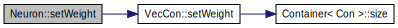
\includegraphics[width=400pt]{class_neuron_ab067bfe507f5386eccc860d4ad2d0bca_cgraph}
\end{center}
\end{figure}


\hypertarget{class_neuron_a255c3597520c730d798218f7174eff1b}{
\index{Neuron@{Neuron}!show@{show}}
\index{show@{show}!Neuron@{Neuron}}
\subsubsection[{show}]{\setlength{\rightskip}{0pt plus 5cm}bool Neuron::show (
\begin{DoxyParamCaption}
{}
\end{DoxyParamCaption}
)}}
\label{class_neuron_a255c3597520c730d798218f7174eff1b}


Definition at line 55 of file Neuron.cpp.



References con, getId(), numOfCons(), and Container$<$ T $>$::show().


\begin{DoxyCode}
                                  {
        int id=getId();
        Rprintf("\n------------------------\n");
        if (id==NA_INTEGER) {
                Rprintf("\n Id: NA, Invalid neuron Id");
        } else {
                Rprintf("\n Id: %d", id);
        }
        Rprintf("\n------------------------\n");
        if (numOfCons()==0) {
                Rprintf("\n No connections defined");
        } else {
                con.show();
        }
        Rprintf("\n------------------------\n");
        return true;

}
\end{DoxyCode}


Here is the call graph for this function:
\nopagebreak
\begin{figure}[H]
\begin{center}
\leavevmode
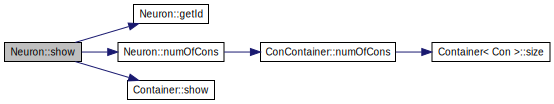
\includegraphics[width=400pt]{class_neuron_a255c3597520c730d798218f7174eff1b_cgraph}
\end{center}
\end{figure}


\hypertarget{class_neuron_a95327aa80a9ec949491f214a0c159b5a}{
\index{Neuron@{Neuron}!validate@{validate}}
\index{validate@{validate}!Neuron@{Neuron}}
\subsubsection[{validate}]{\setlength{\rightskip}{0pt plus 5cm}bool Neuron::validate (
\begin{DoxyParamCaption}
{}
\end{DoxyParamCaption}
)}}
\label{class_neuron_a95327aa80a9ec949491f214a0c159b5a}


Definition at line 75 of file Neuron.cpp.



References con, getId(), and VecCon::validate().


\begin{DoxyCode}
                          {
        BEGIN_RCPP
        if (getId() == NA_INTEGER )             throw std::range_error("[C++ Neur
      on::validate]: Error, Id is NA.");
        con.validate();
        return(TRUE);
        END_RCPP

}
\end{DoxyCode}


Here is the call graph for this function:
\nopagebreak
\begin{figure}[H]
\begin{center}
\leavevmode
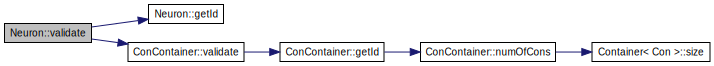
\includegraphics[width=400pt]{class_neuron_a95327aa80a9ec949491f214a0c159b5a_cgraph}
\end{center}
\end{figure}




\subsection{Member Data Documentation}
\hypertarget{class_neuron_a1451f2424a8f9e46ca643d03ff98a616}{
\index{Neuron@{Neuron}!con@{con}}
\index{con@{con}!Neuron@{Neuron}}
\subsubsection[{con}]{\setlength{\rightskip}{0pt plus 5cm}{\bf VecCon} {\bf Neuron::con}\hspace{0.3cm}{\ttfamily  \mbox{[}private\mbox{]}}}}
\label{class_neuron_a1451f2424a8f9e46ca643d03ff98a616}


A vector of input connections. 



Definition at line 28 of file Neuron.h.



Referenced by getConId(), getFrom(), getWeight(), numOfCons(), setFrom(), setWeight(), show(), and validate().

\hypertarget{class_neuron_a72bb327a7c5c865e6748a4e074ce0680}{
\index{Neuron@{Neuron}!Id@{Id}}
\index{Id@{Id}!Neuron@{Neuron}}
\subsubsection[{Id}]{\setlength{\rightskip}{0pt plus 5cm}int {\bf Neuron::Id}\hspace{0.3cm}{\ttfamily  \mbox{[}private\mbox{]}}}}
\label{class_neuron_a72bb327a7c5c865e6748a4e074ce0680}


An integer variable with the \hyperlink{class_neuron}{Neuron} Id. 

The \hyperlink{class_neuron}{Neuron} Id provides a name to the neuron. This value is not expected to be used neither during simulation nor training but it provides an easy reference for human readers. 

Definition at line 21 of file Neuron.h.



Referenced by getId(), and setId().

\hypertarget{class_neuron_ada029047646c36e525a6a1b77cafc03c}{
\index{Neuron@{Neuron}!outputValue@{outputValue}}
\index{outputValue@{outputValue}!Neuron@{Neuron}}
\subsubsection[{outputValue}]{\setlength{\rightskip}{0pt plus 5cm}double {\bf Neuron::outputValue}\hspace{0.3cm}{\ttfamily  \mbox{[}private\mbox{]}}}}
\label{class_neuron_ada029047646c36e525a6a1b77cafc03c}


Definition at line 29 of file Neuron.h.



The documentation for this class was generated from the following files:\begin{DoxyCompactItemize}
\item 
pkg/AMORE/src/\hyperlink{_neuron_8h}{Neuron.h}\item 
pkg/AMORE/src/\hyperlink{_neuron_8cpp}{Neuron.cpp}\end{DoxyCompactItemize}

\hypertarget{class_predict_behavior}{
\section{PredictBehavior Class Reference}
\label{class_predict_behavior}\index{PredictBehavior@{PredictBehavior}}
}


class \hyperlink{class_predict_behavior}{PredictBehavior} -\/  




{\ttfamily \#include $<$PredictBehavior.h$>$}



Inheritance diagram for PredictBehavior:
\nopagebreak
\begin{figure}[H]
\begin{center}
\leavevmode
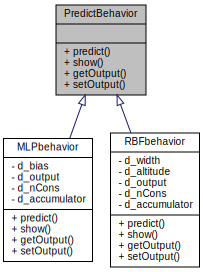
\includegraphics[width=286pt]{class_predict_behavior__inherit__graph}
\end{center}
\end{figure}
\subsection*{Public Member Functions}
\begin{DoxyCompactItemize}
\item 
virtual void \hyperlink{class_predict_behavior_a7db41238d6d1dbf60c67cf8575e79885}{predict} ()=0
\item 
virtual void \hyperlink{class_predict_behavior_a9ef84360f73784248d994fa4707c1dde}{show} ()=0
\item 
double \hyperlink{class_predict_behavior_ac07dbe00c03788119df5df9f57ce11e5}{getOutput} ()
\item 
void \hyperlink{class_predict_behavior_afeabe1f543e46d41909b41816d8210a6}{setOutput} (double output)
\item 
void \hyperlink{class_predict_behavior_a996642f65ce5f5933854039981b66b56}{setActivationFunction} (\hyperlink{_a_m_o_r_e_8h_a77602a0277a02e5769c3df0adc669b17}{ActivationFunctionPtr} activationFunctionPtr, \hyperlink{_a_m_o_r_e_8h_a1fb2f1f8fdf1e08c42ef4bdce436af93}{PredictBehaviorPtr} predictBehaviorPtr)
\item 
double \hyperlink{class_predict_behavior_a69187d626108f96e50675729828daf07}{getInducedLocalField} ()
\item 
void \hyperlink{class_predict_behavior_a0acf1564a1d50771e357dae05986f7b8}{setConnections} (\hyperlink{_a_m_o_r_e_8h_a1021dbaf961d1c8da6d58a8566e5778b}{ConContainerPtr} conContainerPtr)
\end{DoxyCompactItemize}
\subsection*{Protected Member Functions}
\begin{DoxyCompactItemize}
\item 
\hyperlink{class_predict_behavior_af0a2b23a6b860f470a3d7d22ce604689}{PredictBehavior} ()
\end{DoxyCompactItemize}
\subsection*{Protected Attributes}
\begin{DoxyCompactItemize}
\item 
\hyperlink{_a_m_o_r_e_8h_a1021dbaf961d1c8da6d58a8566e5778b}{ConContainerPtr} \hyperlink{class_predict_behavior_ae7d8e531771e06a855f4f1ade167f2f3}{d\_\-nCons}
\item 
double \hyperlink{class_predict_behavior_afdf6139d11c2c1336dd9402262dc1b5e}{d\_\-inducedLocalField}
\item 
\hyperlink{_a_m_o_r_e_8h_a77602a0277a02e5769c3df0adc669b17}{ActivationFunctionPtr} \hyperlink{class_predict_behavior_a60e5bf9ad1d151741a359cdd88346eb5}{d\_\-activationFunction}
\item 
double \hyperlink{class_predict_behavior_acae2a69a47c0af627fc17b9243148db2}{d\_\-output}
\end{DoxyCompactItemize}


\subsection{Detailed Description}
class \hyperlink{class_predict_behavior}{PredictBehavior} -\/ 

Definition at line 4 of file PredictBehavior.h.



\subsection{Constructor \& Destructor Documentation}
\hypertarget{class_predict_behavior_af0a2b23a6b860f470a3d7d22ce604689}{
\index{PredictBehavior@{PredictBehavior}!PredictBehavior@{PredictBehavior}}
\index{PredictBehavior@{PredictBehavior}!PredictBehavior@{PredictBehavior}}
\subsubsection[{PredictBehavior}]{\setlength{\rightskip}{0pt plus 5cm}PredictBehavior::PredictBehavior (
\begin{DoxyParamCaption}
{}
\end{DoxyParamCaption}
)\hspace{0.3cm}{\ttfamily  \mbox{[}protected\mbox{]}}}}
\label{class_predict_behavior_af0a2b23a6b860f470a3d7d22ce604689}


Definition at line 11 of file PredictBehavior.cpp.


\begin{DoxyCode}
                                 :
  d_output(0.0), d_inducedLocalField(0.0)
{
}
\end{DoxyCode}


\subsection{Member Function Documentation}
\hypertarget{class_predict_behavior_a69187d626108f96e50675729828daf07}{
\index{PredictBehavior@{PredictBehavior}!getInducedLocalField@{getInducedLocalField}}
\index{getInducedLocalField@{getInducedLocalField}!PredictBehavior@{PredictBehavior}}
\subsubsection[{getInducedLocalField}]{\setlength{\rightskip}{0pt plus 5cm}double PredictBehavior::getInducedLocalField (
\begin{DoxyParamCaption}
{}
\end{DoxyParamCaption}
)}}
\label{class_predict_behavior_a69187d626108f96e50675729828daf07}


Definition at line 29 of file PredictBehavior.cpp.



References d\_\-inducedLocalField.


\begin{DoxyCode}
{
  return d_inducedLocalField;
}
\end{DoxyCode}
\hypertarget{class_predict_behavior_ac07dbe00c03788119df5df9f57ce11e5}{
\index{PredictBehavior@{PredictBehavior}!getOutput@{getOutput}}
\index{getOutput@{getOutput}!PredictBehavior@{PredictBehavior}}
\subsubsection[{getOutput}]{\setlength{\rightskip}{0pt plus 5cm}double PredictBehavior::getOutput (
\begin{DoxyParamCaption}
{}
\end{DoxyParamCaption}
)}}
\label{class_predict_behavior_ac07dbe00c03788119df5df9f57ce11e5}


Definition at line 23 of file PredictBehavior.cpp.



References d\_\-output.


\begin{DoxyCode}
{
  return d_output;
}
\end{DoxyCode}
\hypertarget{class_predict_behavior_a7db41238d6d1dbf60c67cf8575e79885}{
\index{PredictBehavior@{PredictBehavior}!predict@{predict}}
\index{predict@{predict}!PredictBehavior@{PredictBehavior}}
\subsubsection[{predict}]{\setlength{\rightskip}{0pt plus 5cm}virtual void PredictBehavior::predict (
\begin{DoxyParamCaption}
{}
\end{DoxyParamCaption}
)\hspace{0.3cm}{\ttfamily  \mbox{[}pure virtual\mbox{]}}}}
\label{class_predict_behavior_a7db41238d6d1dbf60c67cf8575e79885}


Implemented in \hyperlink{class_m_l_pbehavior_aaff94adc3577cda9e48d8da925b0ffbf}{MLPbehavior}, and \hyperlink{class_r_b_fbehavior_ac14521848163e04810a6d038aef81896}{RBFbehavior}.

\hypertarget{class_predict_behavior_a996642f65ce5f5933854039981b66b56}{
\index{PredictBehavior@{PredictBehavior}!setActivationFunction@{setActivationFunction}}
\index{setActivationFunction@{setActivationFunction}!PredictBehavior@{PredictBehavior}}
\subsubsection[{setActivationFunction}]{\setlength{\rightskip}{0pt plus 5cm}void PredictBehavior::setActivationFunction (
\begin{DoxyParamCaption}
\item[{{\bf ActivationFunctionPtr}}]{activationFunctionPtr, }
\item[{{\bf PredictBehaviorPtr}}]{predictBehaviorPtr}
\end{DoxyParamCaption}
)}}
\label{class_predict_behavior_a996642f65ce5f5933854039981b66b56}


Definition at line 35 of file PredictBehavior.cpp.



References d\_\-activationFunction.


\begin{DoxyCode}
{
  d_activationFunction = activationFunctionPtr;
  d_activationFunction.get()->setPredictBehavior(predictBehaviorPtr);
}
\end{DoxyCode}
\hypertarget{class_predict_behavior_a0acf1564a1d50771e357dae05986f7b8}{
\index{PredictBehavior@{PredictBehavior}!setConnections@{setConnections}}
\index{setConnections@{setConnections}!PredictBehavior@{PredictBehavior}}
\subsubsection[{setConnections}]{\setlength{\rightskip}{0pt plus 5cm}void PredictBehavior::setConnections (
\begin{DoxyParamCaption}
\item[{{\bf ConContainerPtr}}]{conContainerPtr}
\end{DoxyParamCaption}
)}}
\label{class_predict_behavior_a0acf1564a1d50771e357dae05986f7b8}


Definition at line 44 of file PredictBehavior.cpp.



References d\_\-nCons.


\begin{DoxyCode}
{
  d_nCons = conContainerPtr;
}
\end{DoxyCode}
\hypertarget{class_predict_behavior_afeabe1f543e46d41909b41816d8210a6}{
\index{PredictBehavior@{PredictBehavior}!setOutput@{setOutput}}
\index{setOutput@{setOutput}!PredictBehavior@{PredictBehavior}}
\subsubsection[{setOutput}]{\setlength{\rightskip}{0pt plus 5cm}void PredictBehavior::setOutput (
\begin{DoxyParamCaption}
\item[{double}]{output}
\end{DoxyParamCaption}
)}}
\label{class_predict_behavior_afeabe1f543e46d41909b41816d8210a6}


Definition at line 17 of file PredictBehavior.cpp.



References d\_\-output.


\begin{DoxyCode}
{
  d_output = output;
}
\end{DoxyCode}
\hypertarget{class_predict_behavior_a9ef84360f73784248d994fa4707c1dde}{
\index{PredictBehavior@{PredictBehavior}!show@{show}}
\index{show@{show}!PredictBehavior@{PredictBehavior}}
\subsubsection[{show}]{\setlength{\rightskip}{0pt plus 5cm}virtual void PredictBehavior::show (
\begin{DoxyParamCaption}
{}
\end{DoxyParamCaption}
)\hspace{0.3cm}{\ttfamily  \mbox{[}pure virtual\mbox{]}}}}
\label{class_predict_behavior_a9ef84360f73784248d994fa4707c1dde}


Implemented in \hyperlink{class_m_l_pbehavior_a32aa885e07e8f4eb33e05afb46040567}{MLPbehavior}, and \hyperlink{class_r_b_fbehavior_a96b123a5b657e46946c3ff98ea78f5de}{RBFbehavior}.



\subsection{Member Data Documentation}
\hypertarget{class_predict_behavior_a60e5bf9ad1d151741a359cdd88346eb5}{
\index{PredictBehavior@{PredictBehavior}!d\_\-activationFunction@{d\_\-activationFunction}}
\index{d\_\-activationFunction@{d\_\-activationFunction}!PredictBehavior@{PredictBehavior}}
\subsubsection[{d\_\-activationFunction}]{\setlength{\rightskip}{0pt plus 5cm}{\bf ActivationFunctionPtr} {\bf PredictBehavior::d\_\-activationFunction}\hspace{0.3cm}{\ttfamily  \mbox{[}protected\mbox{]}}}}
\label{class_predict_behavior_a60e5bf9ad1d151741a359cdd88346eb5}


Definition at line 9 of file PredictBehavior.h.



Referenced by MLPbehavior::predict(), and setActivationFunction().

\hypertarget{class_predict_behavior_afdf6139d11c2c1336dd9402262dc1b5e}{
\index{PredictBehavior@{PredictBehavior}!d\_\-inducedLocalField@{d\_\-inducedLocalField}}
\index{d\_\-inducedLocalField@{d\_\-inducedLocalField}!PredictBehavior@{PredictBehavior}}
\subsubsection[{d\_\-inducedLocalField}]{\setlength{\rightskip}{0pt plus 5cm}double {\bf PredictBehavior::d\_\-inducedLocalField}\hspace{0.3cm}{\ttfamily  \mbox{[}protected\mbox{]}}}}
\label{class_predict_behavior_afdf6139d11c2c1336dd9402262dc1b5e}


Definition at line 8 of file PredictBehavior.h.



Referenced by getInducedLocalField(), and MLPbehavior::predict().

\hypertarget{class_predict_behavior_ae7d8e531771e06a855f4f1ade167f2f3}{
\index{PredictBehavior@{PredictBehavior}!d\_\-nCons@{d\_\-nCons}}
\index{d\_\-nCons@{d\_\-nCons}!PredictBehavior@{PredictBehavior}}
\subsubsection[{d\_\-nCons}]{\setlength{\rightskip}{0pt plus 5cm}{\bf ConContainerPtr} {\bf PredictBehavior::d\_\-nCons}\hspace{0.3cm}{\ttfamily  \mbox{[}protected\mbox{]}}}}
\label{class_predict_behavior_ae7d8e531771e06a855f4f1ade167f2f3}


Definition at line 7 of file PredictBehavior.h.



Referenced by MLPbehavior::predict(), setConnections(), and MLPbehavior::show().

\hypertarget{class_predict_behavior_acae2a69a47c0af627fc17b9243148db2}{
\index{PredictBehavior@{PredictBehavior}!d\_\-output@{d\_\-output}}
\index{d\_\-output@{d\_\-output}!PredictBehavior@{PredictBehavior}}
\subsubsection[{d\_\-output}]{\setlength{\rightskip}{0pt plus 5cm}double {\bf PredictBehavior::d\_\-output}\hspace{0.3cm}{\ttfamily  \mbox{[}protected\mbox{]}}}}
\label{class_predict_behavior_acae2a69a47c0af627fc17b9243148db2}


Definition at line 10 of file PredictBehavior.h.



Referenced by getOutput(), MLPbehavior::predict(), setOutput(), and MLPbehavior::show().



The documentation for this class was generated from the following files:\begin{DoxyCompactItemize}
\item 
pkg/AMORE/src/dia/\hyperlink{_predict_behavior_8h}{PredictBehavior.h}\item 
pkg/AMORE/src/\hyperlink{_predict_behavior_8cpp}{PredictBehavior.cpp}\end{DoxyCompactItemize}

\hypertarget{class_r_b_fbehavior}{
\section{RBFbehavior Class Reference}
\label{class_r_b_fbehavior}\index{RBFbehavior@{RBFbehavior}}
}


class \hyperlink{class_r_b_fbehavior}{RBFbehavior} -\/  




{\ttfamily \#include $<$RBFbehavior.h$>$}



Inheritance diagram for RBFbehavior:
\nopagebreak
\begin{figure}[H]
\begin{center}
\leavevmode
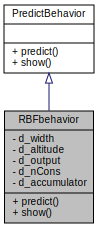
\includegraphics[width=214pt]{class_r_b_fbehavior__inherit__graph}
\end{center}
\end{figure}


Collaboration diagram for RBFbehavior:
\nopagebreak
\begin{figure}[H]
\begin{center}
\leavevmode
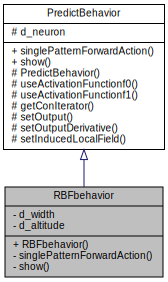
\includegraphics[width=214pt]{class_r_b_fbehavior__coll__graph}
\end{center}
\end{figure}
\subsection*{Public Member Functions}
\begin{DoxyCompactItemize}
\item 
\hyperlink{class_r_b_fbehavior_a647307bf5da0c9c909e7dd1ae92634c9}{RBFbehavior} ()
\item 
void \hyperlink{class_r_b_fbehavior_ac14521848163e04810a6d038aef81896}{predict} ()
\item 
void \hyperlink{class_r_b_fbehavior_a96b123a5b657e46946c3ff98ea78f5de}{show} ()
\end{DoxyCompactItemize}
\subsection*{Private Attributes}
\begin{DoxyCompactItemize}
\item 
double \hyperlink{class_r_b_fbehavior_a6b37a2973f5e8390e37333e81de26077}{d\_\-width}
\item 
double \hyperlink{class_r_b_fbehavior_a831ab08f316756149ff37a92098f7033}{d\_\-altitude}
\end{DoxyCompactItemize}


\subsection{Detailed Description}
class \hyperlink{class_r_b_fbehavior}{RBFbehavior} -\/ 

Definition at line 5 of file RBFbehavior.h.



\subsection{Constructor \& Destructor Documentation}
\hypertarget{class_r_b_fbehavior_a647307bf5da0c9c909e7dd1ae92634c9}{
\index{RBFbehavior@{RBFbehavior}!RBFbehavior@{RBFbehavior}}
\index{RBFbehavior@{RBFbehavior}!RBFbehavior@{RBFbehavior}}
\subsubsection[{RBFbehavior}]{\setlength{\rightskip}{0pt plus 5cm}RBFbehavior::RBFbehavior (
\begin{DoxyParamCaption}
{}
\end{DoxyParamCaption}
)}}
\label{class_r_b_fbehavior_a647307bf5da0c9c909e7dd1ae92634c9}


\subsection{Member Function Documentation}
\hypertarget{class_r_b_fbehavior_ac14521848163e04810a6d038aef81896}{
\index{RBFbehavior@{RBFbehavior}!predict@{predict}}
\index{predict@{predict}!RBFbehavior@{RBFbehavior}}
\subsubsection[{predict}]{\setlength{\rightskip}{0pt plus 5cm}void RBFbehavior::predict (
\begin{DoxyParamCaption}
{}
\end{DoxyParamCaption}
)\hspace{0.3cm}{\ttfamily  \mbox{[}virtual\mbox{]}}}}
\label{class_r_b_fbehavior_ac14521848163e04810a6d038aef81896}


Implements \hyperlink{class_predict_behavior_a7db41238d6d1dbf60c67cf8575e79885}{PredictBehavior}.

\hypertarget{class_r_b_fbehavior_a96b123a5b657e46946c3ff98ea78f5de}{
\index{RBFbehavior@{RBFbehavior}!show@{show}}
\index{show@{show}!RBFbehavior@{RBFbehavior}}
\subsubsection[{show}]{\setlength{\rightskip}{0pt plus 5cm}void RBFbehavior::show (
\begin{DoxyParamCaption}
{}
\end{DoxyParamCaption}
)\hspace{0.3cm}{\ttfamily  \mbox{[}virtual\mbox{]}}}}
\label{class_r_b_fbehavior_a96b123a5b657e46946c3ff98ea78f5de}


Implements \hyperlink{class_predict_behavior_a9ef84360f73784248d994fa4707c1dde}{PredictBehavior}.



\subsection{Member Data Documentation}
\hypertarget{class_r_b_fbehavior_a831ab08f316756149ff37a92098f7033}{
\index{RBFbehavior@{RBFbehavior}!d\_\-altitude@{d\_\-altitude}}
\index{d\_\-altitude@{d\_\-altitude}!RBFbehavior@{RBFbehavior}}
\subsubsection[{d\_\-altitude}]{\setlength{\rightskip}{0pt plus 5cm}double {\bf RBFbehavior::d\_\-altitude}\hspace{0.3cm}{\ttfamily  \mbox{[}private\mbox{]}}}}
\label{class_r_b_fbehavior_a831ab08f316756149ff37a92098f7033}


Definition at line 9 of file RBFbehavior.h.

\hypertarget{class_r_b_fbehavior_a6b37a2973f5e8390e37333e81de26077}{
\index{RBFbehavior@{RBFbehavior}!d\_\-width@{d\_\-width}}
\index{d\_\-width@{d\_\-width}!RBFbehavior@{RBFbehavior}}
\subsubsection[{d\_\-width}]{\setlength{\rightskip}{0pt plus 5cm}double {\bf RBFbehavior::d\_\-width}\hspace{0.3cm}{\ttfamily  \mbox{[}private\mbox{]}}}}
\label{class_r_b_fbehavior_a6b37a2973f5e8390e37333e81de26077}


Definition at line 8 of file RBFbehavior.h.



The documentation for this class was generated from the following file:\begin{DoxyCompactItemize}
\item 
pkg/AMORE/src/dia/\hyperlink{_r_b_fbehavior_8h}{RBFbehavior.h}\end{DoxyCompactItemize}

\hypertarget{class_r_b_ffactory}{
\section{RBFfactory Class Reference}
\label{class_r_b_ffactory}\index{RBFfactory@{RBFfactory}}
}


class \hyperlink{class_r_b_ffactory}{RBFfactory} -\/  




{\ttfamily \#include $<$RBFfactory.h$>$}



Inheritance diagram for RBFfactory:\nopagebreak
\begin{figure}[H]
\begin{center}
\leavevmode
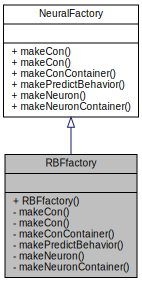
\includegraphics[width=222pt]{class_r_b_ffactory__inherit__graph}
\end{center}
\end{figure}


Collaboration diagram for RBFfactory:\nopagebreak
\begin{figure}[H]
\begin{center}
\leavevmode
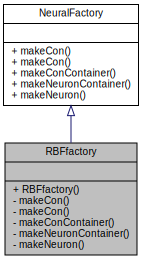
\includegraphics[width=222pt]{class_r_b_ffactory__coll__graph}
\end{center}
\end{figure}
\subsection*{Protected Member Functions}
\begin{DoxyCompactItemize}
\item 
\hyperlink{_a_m_o_r_e_8h_a169bb8e5f26ce70bf2b10dec2fb5ee50}{ConPtr} \hyperlink{class_r_b_ffactory_a5068c3caacf0525f7069dbec4bf87a67}{makeCon} (\hyperlink{class_neuron}{Neuron} $\ast$neuron, double weight)
\item 
\hyperlink{_a_m_o_r_e_8h_a1021dbaf961d1c8da6d58a8566e5778b}{ConContainerPtr} \hyperlink{class_r_b_ffactory_a0b85ec075904a9d915d1a3527f5d6471}{makeConContainer} ()
\item 
virtual \hyperlink{_a_m_o_r_e_8h_a77602a0277a02e5769c3df0adc669b17}{ActivationFunctionPtr} \hyperlink{class_r_b_ffactory_a5620811041643684e164fb19bd03258b}{makeActivationFunction} (\hyperlink{_a_m_o_r_e_8h_ac1ea936c2c7728eb382278131652fef4}{NeuronPtr} neuronPtr)=0
\item 
\hyperlink{_a_m_o_r_e_8h_a1fb2f1f8fdf1e08c42ef4bdce436af93}{PredictBehaviorPtr} \hyperlink{class_r_b_ffactory_a37c1e41af6f362767be462afcd417726}{makePredictBehavior} ()
\item 
\hyperlink{_a_m_o_r_e_8h_ac1ea936c2c7728eb382278131652fef4}{NeuronPtr} \hyperlink{class_r_b_ffactory_a3c6fa334aaffe3ebcbd35da57e6ce045}{makeNeuron} (\hyperlink{_a_m_o_r_e_8h_abc871abb71cff6655b8172ee7240b8ef}{Handler} Id)
\item 
\hyperlink{_a_m_o_r_e_8h_ac1ea936c2c7728eb382278131652fef4}{NeuronPtr} \hyperlink{class_r_b_ffactory_a244d2f6eb8d7d36b1fc5252ab10797ed}{makeNeuron} (\hyperlink{_a_m_o_r_e_8h_abc871abb71cff6655b8172ee7240b8ef}{Handler} Id, \hyperlink{_a_m_o_r_e_8h_aa794539c0a68e4eb451e7a2cc6294acc}{NeuronIteratorPtr} neuronIteratorPtr, double totalAmountOfParameters)
\item 
\hyperlink{_a_m_o_r_e_8h_acce4b66db3921b7326fbe1a04a56e5fc}{LayerPtr} \hyperlink{class_r_b_ffactory_a6ad31da66b1e633de65bca9e2b6e79c2}{makeLayer} ()
\item 
\hyperlink{_a_m_o_r_e_8h_af261b546158af61fc27686fb926961f2}{LayerContainerPtr} \hyperlink{class_r_b_ffactory_a2f66a1e1b09b4cfffeb4972a4d8b0a3c}{makeLayerContainer} ()
\item 
\hyperlink{_a_m_o_r_e_8h_a7adadf1c313313507b00cd1193db29a1}{NeuralNetworkPtr} \hyperlink{class_r_b_ffactory_a73207bed1447c8b1f5b1c8ecd3dc0d16}{makeNeuralNetwork} (\hyperlink{class_neural_factory}{NeuralFactory} \&neuralFactory)
\item 
\hyperlink{_a_m_o_r_e_8h_aefebabe3353f684b7708712480c15699}{NeuralCreatorPtr} \hyperlink{class_r_b_ffactory_a458d59688c8fb27ee5f9206f248dca03}{makeNeuralCreator} ()
\end{DoxyCompactItemize}


\subsection{Detailed Description}
class \hyperlink{class_r_b_ffactory}{RBFfactory} -\/ 

Definition at line 5 of file RBFfactory.h.



\subsection{Member Function Documentation}
\hypertarget{class_r_b_ffactory_a5620811041643684e164fb19bd03258b}{
\index{RBFfactory@{RBFfactory}!makeActivationFunction@{makeActivationFunction}}
\index{makeActivationFunction@{makeActivationFunction}!RBFfactory@{RBFfactory}}
\subsubsection[{makeActivationFunction}]{\setlength{\rightskip}{0pt plus 5cm}virtual {\bf ActivationFunctionPtr} RBFfactory::makeActivationFunction (
\begin{DoxyParamCaption}
\item[{{\bf NeuronPtr}}]{neuronPtr}
\end{DoxyParamCaption}
)\hspace{0.3cm}{\ttfamily  \mbox{[}protected, pure virtual\mbox{]}}}}
\label{class_r_b_ffactory_a5620811041643684e164fb19bd03258b}


Implements \hyperlink{class_neural_factory_a678ec16456e5772a2c188c475a78c588}{NeuralFactory}.



Implemented in \hyperlink{class_radial_basis_factory_ae68ec682e8f04e99e5a1560e347b7735}{RadialBasisFactory}.

\hypertarget{class_r_b_ffactory_a5068c3caacf0525f7069dbec4bf87a67}{
\index{RBFfactory@{RBFfactory}!makeCon@{makeCon}}
\index{makeCon@{makeCon}!RBFfactory@{RBFfactory}}
\subsubsection[{makeCon}]{\setlength{\rightskip}{0pt plus 5cm}{\bf ConPtr} RBFfactory::makeCon (
\begin{DoxyParamCaption}
\item[{{\bf Neuron} $\ast$}]{neuron, }
\item[{double}]{weight}
\end{DoxyParamCaption}
)\hspace{0.3cm}{\ttfamily  \mbox{[}protected\mbox{]}}}}
\label{class_r_b_ffactory_a5068c3caacf0525f7069dbec4bf87a67}
\hypertarget{class_r_b_ffactory_a0b85ec075904a9d915d1a3527f5d6471}{
\index{RBFfactory@{RBFfactory}!makeConContainer@{makeConContainer}}
\index{makeConContainer@{makeConContainer}!RBFfactory@{RBFfactory}}
\subsubsection[{makeConContainer}]{\setlength{\rightskip}{0pt plus 5cm}{\bf ConContainerPtr} RBFfactory::makeConContainer (
\begin{DoxyParamCaption}
{}
\end{DoxyParamCaption}
)\hspace{0.3cm}{\ttfamily  \mbox{[}protected, virtual\mbox{]}}}}
\label{class_r_b_ffactory_a0b85ec075904a9d915d1a3527f5d6471}


Implements \hyperlink{class_neural_factory_a4fa5f4f57a2551c95481146b1a0c83d7}{NeuralFactory}.

\hypertarget{class_r_b_ffactory_a6ad31da66b1e633de65bca9e2b6e79c2}{
\index{RBFfactory@{RBFfactory}!makeLayer@{makeLayer}}
\index{makeLayer@{makeLayer}!RBFfactory@{RBFfactory}}
\subsubsection[{makeLayer}]{\setlength{\rightskip}{0pt plus 5cm}{\bf LayerPtr} RBFfactory::makeLayer (
\begin{DoxyParamCaption}
{}
\end{DoxyParamCaption}
)\hspace{0.3cm}{\ttfamily  \mbox{[}protected, virtual\mbox{]}}}}
\label{class_r_b_ffactory_a6ad31da66b1e633de65bca9e2b6e79c2}


Implements \hyperlink{class_neural_factory_a1a02bc2427430c4085654a72a03a5f4f}{NeuralFactory}.

\hypertarget{class_r_b_ffactory_a2f66a1e1b09b4cfffeb4972a4d8b0a3c}{
\index{RBFfactory@{RBFfactory}!makeLayerContainer@{makeLayerContainer}}
\index{makeLayerContainer@{makeLayerContainer}!RBFfactory@{RBFfactory}}
\subsubsection[{makeLayerContainer}]{\setlength{\rightskip}{0pt plus 5cm}{\bf LayerContainerPtr} RBFfactory::makeLayerContainer (
\begin{DoxyParamCaption}
{}
\end{DoxyParamCaption}
)\hspace{0.3cm}{\ttfamily  \mbox{[}protected, virtual\mbox{]}}}}
\label{class_r_b_ffactory_a2f66a1e1b09b4cfffeb4972a4d8b0a3c}


Implements \hyperlink{class_neural_factory_a10b5056a57cc3fef56c66da1ad367fc7}{NeuralFactory}.

\hypertarget{class_r_b_ffactory_a458d59688c8fb27ee5f9206f248dca03}{
\index{RBFfactory@{RBFfactory}!makeNeuralCreator@{makeNeuralCreator}}
\index{makeNeuralCreator@{makeNeuralCreator}!RBFfactory@{RBFfactory}}
\subsubsection[{makeNeuralCreator}]{\setlength{\rightskip}{0pt plus 5cm}{\bf NeuralCreatorPtr} RBFfactory::makeNeuralCreator (
\begin{DoxyParamCaption}
{}
\end{DoxyParamCaption}
)\hspace{0.3cm}{\ttfamily  \mbox{[}protected, virtual\mbox{]}}}}
\label{class_r_b_ffactory_a458d59688c8fb27ee5f9206f248dca03}


Implements \hyperlink{class_neural_factory_a2c7502e1bf81d3fc33284123d733428e}{NeuralFactory}.

\hypertarget{class_r_b_ffactory_a73207bed1447c8b1f5b1c8ecd3dc0d16}{
\index{RBFfactory@{RBFfactory}!makeNeuralNetwork@{makeNeuralNetwork}}
\index{makeNeuralNetwork@{makeNeuralNetwork}!RBFfactory@{RBFfactory}}
\subsubsection[{makeNeuralNetwork}]{\setlength{\rightskip}{0pt plus 5cm}{\bf NeuralNetworkPtr} RBFfactory::makeNeuralNetwork (
\begin{DoxyParamCaption}
\item[{{\bf NeuralFactory} \&}]{neuralFactory}
\end{DoxyParamCaption}
)\hspace{0.3cm}{\ttfamily  \mbox{[}protected, virtual\mbox{]}}}}
\label{class_r_b_ffactory_a73207bed1447c8b1f5b1c8ecd3dc0d16}


Implements \hyperlink{class_neural_factory_a15b9308e868ca439869b1d68afabfcde}{NeuralFactory}.

\hypertarget{class_r_b_ffactory_a3c6fa334aaffe3ebcbd35da57e6ce045}{
\index{RBFfactory@{RBFfactory}!makeNeuron@{makeNeuron}}
\index{makeNeuron@{makeNeuron}!RBFfactory@{RBFfactory}}
\subsubsection[{makeNeuron}]{\setlength{\rightskip}{0pt plus 5cm}{\bf NeuronPtr} RBFfactory::makeNeuron (
\begin{DoxyParamCaption}
\item[{{\bf Handler}}]{Id}
\end{DoxyParamCaption}
)\hspace{0.3cm}{\ttfamily  \mbox{[}protected, virtual\mbox{]}}}}
\label{class_r_b_ffactory_a3c6fa334aaffe3ebcbd35da57e6ce045}


Implements \hyperlink{class_neural_factory_a12abbf93f829aab585975f157c8c98f7}{NeuralFactory}.

\hypertarget{class_r_b_ffactory_a244d2f6eb8d7d36b1fc5252ab10797ed}{
\index{RBFfactory@{RBFfactory}!makeNeuron@{makeNeuron}}
\index{makeNeuron@{makeNeuron}!RBFfactory@{RBFfactory}}
\subsubsection[{makeNeuron}]{\setlength{\rightskip}{0pt plus 5cm}{\bf NeuronPtr} RBFfactory::makeNeuron (
\begin{DoxyParamCaption}
\item[{{\bf Handler}}]{Id, }
\item[{{\bf NeuronIteratorPtr}}]{neuronIteratorPtr, }
\item[{double}]{totalAmountOfParameters}
\end{DoxyParamCaption}
)\hspace{0.3cm}{\ttfamily  \mbox{[}protected, virtual\mbox{]}}}}
\label{class_r_b_ffactory_a244d2f6eb8d7d36b1fc5252ab10797ed}


Implements \hyperlink{class_neural_factory_a19c08ba7ad05ef7af05f7595dda2100b}{NeuralFactory}.

\hypertarget{class_r_b_ffactory_a37c1e41af6f362767be462afcd417726}{
\index{RBFfactory@{RBFfactory}!makePredictBehavior@{makePredictBehavior}}
\index{makePredictBehavior@{makePredictBehavior}!RBFfactory@{RBFfactory}}
\subsubsection[{makePredictBehavior}]{\setlength{\rightskip}{0pt plus 5cm}{\bf PredictBehaviorPtr} RBFfactory::makePredictBehavior (
\begin{DoxyParamCaption}
{}
\end{DoxyParamCaption}
)\hspace{0.3cm}{\ttfamily  \mbox{[}protected\mbox{]}}}}
\label{class_r_b_ffactory_a37c1e41af6f362767be462afcd417726}


The documentation for this class was generated from the following file:\begin{DoxyCompactItemize}
\item 
/Users/mcasl/pc-\/ule/Trabajo/investigacion/AMORE/AMORE-\/WC/AMORE-\/WC/pkg/AMORE/src/classHeaders/\hyperlink{_r_b_ffactory_8h}{RBFfactory.h}\end{DoxyCompactItemize}

\hypertarget{class_simple_container}{
\section{SimpleContainer$<$ T $>$ Class Template Reference}
\label{class_simple_container}\index{SimpleContainer@{SimpleContainer}}
}


class \hyperlink{class_simple_container}{SimpleContainer} -\/  




{\ttfamily \#include $<$SimpleContainer.h$>$}



Inheritance diagram for SimpleContainer$<$ T $>$:
\nopagebreak
\begin{figure}[H]
\begin{center}
\leavevmode
\includegraphics[height=600pt]{class_simple_container__inherit__graph}
\end{center}
\end{figure}


Collaboration diagram for SimpleContainer$<$ T $>$:
\nopagebreak
\begin{figure}[H]
\begin{center}
\leavevmode
\includegraphics[height=600pt]{class_simple_container__coll__graph}
\end{center}
\end{figure}
\subsection*{Public Member Functions}
\begin{DoxyCompactItemize}
\item 
\hyperlink{class_simple_container_a87d087aab51b4b6aad359ad906a90e4d}{SimpleContainer} ()
\item 
\hyperlink{class_simple_container_ad0704bf9c306ab57a9c4a2b83879670c}{$\sim$SimpleContainer} ()
\end{DoxyCompactItemize}
\subsection*{Protected Attributes}
\begin{DoxyCompactItemize}
\item 
std::vector$<$ T $>$ \hyperlink{class_simple_container_a0be5592282fc09b51a344d4083a7daf9}{d\_\-collection}
\end{DoxyCompactItemize}
\subsection*{Private Member Functions}
\begin{DoxyCompactItemize}
\item 
boost::shared\_\-ptr$<$ \hyperlink{class_iterator}{Iterator}$<$ T $>$ $>$ \hyperlink{class_simple_container_a4e46f5cb32231deaf9aa9bb7f871d09e}{createIterator} ()
\item 
void \hyperlink{class_simple_container_a53466966297b3f0a707e025b3721004a}{push\_\-back} (T const \&\hyperlink{class_container_a8dd7ae9d0687e11d873f98206e961ac1}{const\_\-reference})
\begin{DoxyCompactList}\small\item\em Append a shared\_\-ptr at the end of collection. \end{DoxyCompactList}\item 
void \hyperlink{class_simple_container_a4bca44e6a9cef9d57627218c0a180d8a}{reserve} (int n)
\item 
bool \hyperlink{class_simple_container_ac2966f33796f69c290a84361a578ed08}{empty} ()
\item 
size\_\-type \hyperlink{class_simple_container_a2fdb3580e1728e6e2ba6ef77c0bce63e}{size} ()
\begin{DoxyCompactList}\small\item\em Returns the size or length of the vector. \end{DoxyCompactList}\item 
void \hyperlink{class_simple_container_ae3ee6cb18f1dd33ab5de4f9854ce245f}{clear} ()
\item 
void \hyperlink{class_simple_container_af4d591e2c3a44ae016e01e3d07d1e9ac}{show} ()
\begin{DoxyCompactList}\small\item\em Pretty print of the Container$<$T$>$ \end{DoxyCompactList}\item 
bool \hyperlink{class_simple_container_ac7cae8eaac2dc0a69138b65f679bd16a}{validate} ()
\begin{DoxyCompactList}\small\item\em Object validator. \end{DoxyCompactList}\end{DoxyCompactItemize}
\subsection*{Friends}
\begin{DoxyCompactItemize}
\item 
class \hyperlink{class_simple_container_a9abe836547cca50b94869af58a0901f7}{SimpleContainerIterator$<$ T $>$}
\end{DoxyCompactItemize}


\subsection{Detailed Description}
\subsubsection*{template$<$typename T$>$class SimpleContainer$<$ T $>$}

class \hyperlink{class_simple_container}{SimpleContainer} -\/ 

Definition at line 6 of file SimpleContainer.h.



\subsection{Constructor \& Destructor Documentation}
\hypertarget{class_simple_container_a87d087aab51b4b6aad359ad906a90e4d}{
\index{SimpleContainer@{SimpleContainer}!SimpleContainer@{SimpleContainer}}
\index{SimpleContainer@{SimpleContainer}!SimpleContainer@{SimpleContainer}}
\subsubsection[{SimpleContainer}]{\setlength{\rightskip}{0pt plus 5cm}template$<$typename T $>$ {\bf SimpleContainer}$<$ T $>$::{\bf SimpleContainer} (
\begin{DoxyParamCaption}
{}
\end{DoxyParamCaption}
)}}
\label{class_simple_container_a87d087aab51b4b6aad359ad906a90e4d}
\hypertarget{class_simple_container_ad0704bf9c306ab57a9c4a2b83879670c}{
\index{SimpleContainer@{SimpleContainer}!$\sim$SimpleContainer@{$\sim$SimpleContainer}}
\index{$\sim$SimpleContainer@{$\sim$SimpleContainer}!SimpleContainer@{SimpleContainer}}
\subsubsection[{$\sim$SimpleContainer}]{\setlength{\rightskip}{0pt plus 5cm}template$<$typename T $>$ {\bf SimpleContainer}$<$ T $>$::$\sim${\bf SimpleContainer} (
\begin{DoxyParamCaption}
{}
\end{DoxyParamCaption}
)}}
\label{class_simple_container_ad0704bf9c306ab57a9c4a2b83879670c}


\subsection{Member Function Documentation}
\hypertarget{class_simple_container_ae3ee6cb18f1dd33ab5de4f9854ce245f}{
\index{SimpleContainer@{SimpleContainer}!clear@{clear}}
\index{clear@{clear}!SimpleContainer@{SimpleContainer}}
\subsubsection[{clear}]{\setlength{\rightskip}{0pt plus 5cm}template$<$typename T $>$ void {\bf SimpleContainer}$<$ T $>$::clear (
\begin{DoxyParamCaption}
{}
\end{DoxyParamCaption}
)\hspace{0.3cm}{\ttfamily  \mbox{[}private, virtual\mbox{]}}}}
\label{class_simple_container_ae3ee6cb18f1dd33ab5de4f9854ce245f}


Implements \hyperlink{class_container_a3c98faf8d85775ce5deb9db00fc11b18}{Container$<$ T $>$}.

\hypertarget{class_simple_container_a4e46f5cb32231deaf9aa9bb7f871d09e}{
\index{SimpleContainer@{SimpleContainer}!createIterator@{createIterator}}
\index{createIterator@{createIterator}!SimpleContainer@{SimpleContainer}}
\subsubsection[{createIterator}]{\setlength{\rightskip}{0pt plus 5cm}template$<$typename T $>$ boost::shared\_\-ptr$<$ {\bf Iterator}$<$T$>$ $>$ {\bf SimpleContainer}$<$ T $>$::createIterator (
\begin{DoxyParamCaption}
{}
\end{DoxyParamCaption}
)\hspace{0.3cm}{\ttfamily  \mbox{[}private, virtual\mbox{]}}}}
\label{class_simple_container_a4e46f5cb32231deaf9aa9bb7f871d09e}


Implements \hyperlink{class_container_a1cfd60c48bf7ac7d0c6e323c8fa3d1da}{Container$<$ T $>$}.

\hypertarget{class_simple_container_ac2966f33796f69c290a84361a578ed08}{
\index{SimpleContainer@{SimpleContainer}!empty@{empty}}
\index{empty@{empty}!SimpleContainer@{SimpleContainer}}
\subsubsection[{empty}]{\setlength{\rightskip}{0pt plus 5cm}template$<$typename T $>$ bool {\bf SimpleContainer}$<$ T $>$::empty (
\begin{DoxyParamCaption}
{}
\end{DoxyParamCaption}
)\hspace{0.3cm}{\ttfamily  \mbox{[}private, virtual\mbox{]}}}}
\label{class_simple_container_ac2966f33796f69c290a84361a578ed08}


Implements \hyperlink{class_container_aeb0ba9c87519ae6b7036d72589948755}{Container$<$ T $>$}.

\hypertarget{class_simple_container_a53466966297b3f0a707e025b3721004a}{
\index{SimpleContainer@{SimpleContainer}!push\_\-back@{push\_\-back}}
\index{push\_\-back@{push\_\-back}!SimpleContainer@{SimpleContainer}}
\subsubsection[{push\_\-back}]{\setlength{\rightskip}{0pt plus 5cm}template$<$typename T $>$ void {\bf SimpleContainer}$<$ T $>$::push\_\-back (
\begin{DoxyParamCaption}
\item[{T const \&}]{reference}
\end{DoxyParamCaption}
)\hspace{0.3cm}{\ttfamily  \mbox{[}private, virtual\mbox{]}}}}
\label{class_simple_container_a53466966297b3f0a707e025b3721004a}


Append a shared\_\-ptr at the end of collection. 

Implements push\_\-back for the \hyperlink{class_container}{Container} class 
\begin{DoxyParams}{Parameters}
{\em TsharedPtr} & A shared\_\-ptr pointer to be inserted at the end of collection\\
\hline
\end{DoxyParams}

\begin{DoxyCode}
                //================
                //Usage example:
                //================
                // Data set up
                        Neuron N1, N2, N3;
                        Container<Con> conContainer;
                        std::vector<ConPtr> vc;
                        std::vector<int> result;
                        N1.setId(10);
                        N2.setId(20);
                        N3.setId(30);
                // Test
                        ConPtr ptCon( new Con(&N1, 1.13) );     // Create new Con
       and initialize ptCon
                        conContainer.push_back(ptCon);                          /
      / push_back
                        ptCon.reset(  new Con(&N2, 2.22) );             // create
       new Con and assign to ptCon
                        conContainer.push_back(ptCon);                          /
      / push_back
                        ptCon.reset(  new Con(&N3, 3.33) );             // create
       new Con and assign to ptCon
                        conContainer.push_back(ptCon);                          /
      / push_back

                        vc = conContainer.load();

                        result.push_back(vc.at(0)->getId());
                        result.push_back(vc.at(1)->getId());
                        result.push_back(vc.at(2)->getId());
        // After execution of this code, result contains a numeric vector with va
      lues 10, 20 and 30.
\end{DoxyCode}


\begin{DoxySeeAlso}{See also}
C++ documentation for std::vector::push\_\-back and the unit test files, e.g., runit.Cpp.Container.R, for usage examples. 
\end{DoxySeeAlso}


Implements \hyperlink{class_container_adc177ce7c428ded8788bc66fb829db8b}{Container$<$ T $>$}.

\hypertarget{class_simple_container_a4bca44e6a9cef9d57627218c0a180d8a}{
\index{SimpleContainer@{SimpleContainer}!reserve@{reserve}}
\index{reserve@{reserve}!SimpleContainer@{SimpleContainer}}
\subsubsection[{reserve}]{\setlength{\rightskip}{0pt plus 5cm}template$<$typename T $>$ void {\bf SimpleContainer}$<$ T $>$::reserve (
\begin{DoxyParamCaption}
\item[{int}]{n}
\end{DoxyParamCaption}
)\hspace{0.3cm}{\ttfamily  \mbox{[}private, virtual\mbox{]}}}}
\label{class_simple_container_a4bca44e6a9cef9d57627218c0a180d8a}


Implements \hyperlink{class_container_a39dd135ff6d4ba1bb3785100e266a748}{Container$<$ T $>$}.

\hypertarget{class_simple_container_af4d591e2c3a44ae016e01e3d07d1e9ac}{
\index{SimpleContainer@{SimpleContainer}!show@{show}}
\index{show@{show}!SimpleContainer@{SimpleContainer}}
\subsubsection[{show}]{\setlength{\rightskip}{0pt plus 5cm}template$<$typename T $>$ void {\bf SimpleContainer}$<$ T $>$::show (
\begin{DoxyParamCaption}
{}
\end{DoxyParamCaption}
)\hspace{0.3cm}{\ttfamily  \mbox{[}private, virtual\mbox{]}}}}
\label{class_simple_container_af4d591e2c3a44ae016e01e3d07d1e9ac}


Pretty print of the Container$<$T$>$ 

This method outputs in the R terminal the contents of \hyperlink{class_container_a6cc12233bceb7d72709320d2c57e3398}{Container::collection}. \begin{DoxyReturn}{Returns}
true in case everything works without throwing an exception
\end{DoxyReturn}
$\ast$ 
\begin{DoxyCode}
                //================
                //Usage example:
                //================
                // Data set up
                        ContainerNeuronPtr      neuronContainerPtr( new 
      Container<Neuron>() );
                        ContainerConPtr conContainerPtr( new Container<Con>() );
                        ConPtr  ptC;
                        NeuronPtr ptN;
                        int ids[]= {10, 20, 30};
                        double weights[] = {1.13, 2.22, 3.33 };

                        for (int i=0; i<=2 ; i++) {                             /
      / Let's create a vector with three neurons
                                ptN.reset( new Neuron( ids[i] ) );
                                neuronContainerPtr->push_back(ptN);
                        }

                        for (int i=0; i<=2 ; i++) {                             /
      / and a vector with three connections
                                ptC.reset( new Con( neuronContainerPtr->load().at
      (i), weights[i]) );
                                conContainerPtr->push_back(ptC);
                        }

                // Test
                        conContainerPtr->show() ;

                // The output at the R terminal would display:
                //
                //      # From:  10      Weight=         1.130000
                //      # From:  20      Weight=         2.220000
                //      # From:  30      Weight=         3.330000
                //
\end{DoxyCode}


\begin{DoxySeeAlso}{See also}
The unit test files, e.g., runit.Cpp.Container.R, for usage examples. 
\end{DoxySeeAlso}


Implements \hyperlink{class_container_ada156e5601bc75549e64ea4befb136f0}{Container$<$ T $>$}.

\hypertarget{class_simple_container_a2fdb3580e1728e6e2ba6ef77c0bce63e}{
\index{SimpleContainer@{SimpleContainer}!size@{size}}
\index{size@{size}!SimpleContainer@{SimpleContainer}}
\subsubsection[{size}]{\setlength{\rightskip}{0pt plus 5cm}template$<$typename T $>$ size\_\-type {\bf SimpleContainer}$<$ T $>$::size (
\begin{DoxyParamCaption}
{}
\end{DoxyParamCaption}
)\hspace{0.3cm}{\ttfamily  \mbox{[}private, virtual\mbox{]}}}}
\label{class_simple_container_a2fdb3580e1728e6e2ba6ef77c0bce63e}


Returns the size or length of the vector. 

This method returns the size of the vector. In the classes derived from Container$<$T$>$ this is aliased as numOfCons, numOfNeurons and numOfLayers. The unit test files, e.g., runit.Cpp.Container.R, for usage examples. 

Implements \hyperlink{class_container_a359f34bc418575b474184cbe3f33527e}{Container$<$ T $>$}.

\hypertarget{class_simple_container_ac7cae8eaac2dc0a69138b65f679bd16a}{
\index{SimpleContainer@{SimpleContainer}!validate@{validate}}
\index{validate@{validate}!SimpleContainer@{SimpleContainer}}
\subsubsection[{validate}]{\setlength{\rightskip}{0pt plus 5cm}template$<$typename T $>$ bool {\bf SimpleContainer}$<$ T $>$::validate (
\begin{DoxyParamCaption}
{}
\end{DoxyParamCaption}
)\hspace{0.3cm}{\ttfamily  \mbox{[}private, virtual\mbox{]}}}}
\label{class_simple_container_ac7cae8eaac2dc0a69138b65f679bd16a}


Object validator. 

This method checks the object for internal coherence. This method calls the validate method for each element in collection, \begin{DoxySeeAlso}{See also}
The unit test files, e.g., runit.Cpp.Container.R, for usage examples. 
\end{DoxySeeAlso}


Implements \hyperlink{class_container_acfdc5456a2fc854d1830a8a351567928}{Container$<$ T $>$}.



\subsection{Friends And Related Function Documentation}
\hypertarget{class_simple_container_a9abe836547cca50b94869af58a0901f7}{
\index{SimpleContainer@{SimpleContainer}!SimpleContainerIterator$<$ T $>$@{SimpleContainerIterator$<$ T $>$}}
\index{SimpleContainerIterator$<$ T $>$@{SimpleContainerIterator$<$ T $>$}!SimpleContainer@{SimpleContainer}}
\subsubsection[{SimpleContainerIterator$<$ T $>$}]{\setlength{\rightskip}{0pt plus 5cm}template$<$typename T $>$ friend class {\bf SimpleContainerIterator}$<$ T $>$\hspace{0.3cm}{\ttfamily  \mbox{[}friend\mbox{]}}}}
\label{class_simple_container_a9abe836547cca50b94869af58a0901f7}


Definition at line 12 of file SimpleContainer.h.



\subsection{Member Data Documentation}
\hypertarget{class_simple_container_a0be5592282fc09b51a344d4083a7daf9}{
\index{SimpleContainer@{SimpleContainer}!d\_\-collection@{d\_\-collection}}
\index{d\_\-collection@{d\_\-collection}!SimpleContainer@{SimpleContainer}}
\subsubsection[{d\_\-collection}]{\setlength{\rightskip}{0pt plus 5cm}template$<$typename T $>$ std::vector$<$ T $>$ {\bf SimpleContainer}$<$ T $>$::{\bf d\_\-collection}\hspace{0.3cm}{\ttfamily  \mbox{[}protected\mbox{]}}}}
\label{class_simple_container_a0be5592282fc09b51a344d4083a7daf9}


Definition at line 9 of file SimpleContainer.h.



The documentation for this class was generated from the following file:\begin{DoxyCompactItemize}
\item 
pkg/AMORE/src/dia/\hyperlink{_simple_container_8h}{SimpleContainer.h}\end{DoxyCompactItemize}

\hypertarget{class_simple_container_iterator}{
\section{SimpleContainerIterator$<$ T $>$ Class Template Reference}
\label{class_simple_container_iterator}\index{SimpleContainerIterator@{SimpleContainerIterator}}
}


class \hyperlink{class_simple_container_iterator}{SimpleContainerIterator} -\/  




{\ttfamily \#include $<$SimpleContainerIterator.h$>$}



Inheritance diagram for SimpleContainerIterator$<$ T $>$:\nopagebreak
\begin{figure}[H]
\begin{center}
\leavevmode
\includegraphics[width=230pt]{class_simple_container_iterator__inherit__graph}
\end{center}
\end{figure}


Collaboration diagram for SimpleContainerIterator$<$ T $>$:\nopagebreak
\begin{figure}[H]
\begin{center}
\leavevmode
\includegraphics[width=230pt]{class_simple_container_iterator__coll__graph}
\end{center}
\end{figure}
\subsection*{Public Member Functions}
\begin{DoxyCompactItemize}
\item 
\hyperlink{class_simple_container_iterator_a7efe60ad1b976260e29cfc793b9f5b1a}{SimpleContainerIterator} ()
\item 
\hyperlink{class_simple_container_iterator_a4f1d34a0c187f4359885755372b6aa79}{$\sim$SimpleContainerIterator} ()
\end{DoxyCompactItemize}
\subsection*{Private Member Functions}
\begin{DoxyCompactItemize}
\item 
void \hyperlink{class_simple_container_iterator_a71b26d5acddcab75ca0386c187fd2bbc}{first} ()
\item 
void \hyperlink{class_simple_container_iterator_a11274af2bc4dc9930f983b7b246d8f87}{next} ()
\item 
bool \hyperlink{class_simple_container_iterator_a91352e803f39fb58d9312d9d866842c8}{isDone} ()
\item 
T \hyperlink{class_simple_container_iterator_ad65642e6d9540b58193e7a40f1688fc7}{currentItem} ()
\end{DoxyCompactItemize}
\subsection*{Private Attributes}
\begin{DoxyCompactItemize}
\item 
\hyperlink{class_container}{Container}$<$ T $>$ $\ast$ \hyperlink{class_simple_container_iterator_a179c3b6ee590cd5476d6dee1c7b9a90e}{d\_\-container}
\item 
size\_\-type \hyperlink{class_simple_container_iterator_a0e03fa66760ef1cb70ed2a357299605f}{d\_\-current}
\end{DoxyCompactItemize}
\subsection*{Friends}
\begin{DoxyCompactItemize}
\item 
class \hyperlink{class_simple_container_iterator_af3eda3b215741021fb668d573cf344f3}{SimpleContainer$<$ T $>$}
\end{DoxyCompactItemize}


\subsection{Detailed Description}
\subsubsection*{template$<$typename T$>$class SimpleContainerIterator$<$ T $>$}

class \hyperlink{class_simple_container_iterator}{SimpleContainerIterator} -\/ 

Definition at line 6 of file SimpleContainerIterator.h.



\subsection{Constructor \& Destructor Documentation}
\hypertarget{class_simple_container_iterator_a7efe60ad1b976260e29cfc793b9f5b1a}{
\index{SimpleContainerIterator@{SimpleContainerIterator}!SimpleContainerIterator@{SimpleContainerIterator}}
\index{SimpleContainerIterator@{SimpleContainerIterator}!SimpleContainerIterator@{SimpleContainerIterator}}
\subsubsection[{SimpleContainerIterator}]{\setlength{\rightskip}{0pt plus 5cm}template$<$typename T $>$ {\bf SimpleContainerIterator}$<$ T $>$::{\bf SimpleContainerIterator} (
\begin{DoxyParamCaption}
{}
\end{DoxyParamCaption}
)}}
\label{class_simple_container_iterator_a7efe60ad1b976260e29cfc793b9f5b1a}


Definition at line 4 of file SimpleContainerIterator.cpp.


\begin{DoxyCode}
  {
  }
\end{DoxyCode}
\hypertarget{class_simple_container_iterator_a4f1d34a0c187f4359885755372b6aa79}{
\index{SimpleContainerIterator@{SimpleContainerIterator}!$\sim$SimpleContainerIterator@{$\sim$SimpleContainerIterator}}
\index{$\sim$SimpleContainerIterator@{$\sim$SimpleContainerIterator}!SimpleContainerIterator@{SimpleContainerIterator}}
\subsubsection[{$\sim$SimpleContainerIterator}]{\setlength{\rightskip}{0pt plus 5cm}template$<$typename T $>$ {\bf SimpleContainerIterator}$<$ T $>$::$\sim${\bf SimpleContainerIterator} (
\begin{DoxyParamCaption}
{}
\end{DoxyParamCaption}
)}}
\label{class_simple_container_iterator_a4f1d34a0c187f4359885755372b6aa79}


Definition at line 9 of file SimpleContainerIterator.cpp.


\begin{DoxyCode}
  {
  }
\end{DoxyCode}


\subsection{Member Function Documentation}
\hypertarget{class_simple_container_iterator_ad65642e6d9540b58193e7a40f1688fc7}{
\index{SimpleContainerIterator@{SimpleContainerIterator}!currentItem@{currentItem}}
\index{currentItem@{currentItem}!SimpleContainerIterator@{SimpleContainerIterator}}
\subsubsection[{currentItem}]{\setlength{\rightskip}{0pt plus 5cm}template$<$typename T $>$ T {\bf SimpleContainerIterator}$<$ T $>$::currentItem (
\begin{DoxyParamCaption}
{}
\end{DoxyParamCaption}
)\hspace{0.3cm}{\ttfamily  \mbox{[}private, virtual\mbox{]}}}}
\label{class_simple_container_iterator_ad65642e6d9540b58193e7a40f1688fc7}


Implements \hyperlink{class_iterator_a1fce5bc9b2218407b5cedf2a0ba3131b}{Iterator$<$ T $>$}.



Definition at line 37 of file SimpleContainerIterator.cpp.


\begin{DoxyCode}
  {
      if (isDone()) throw std::range_error("SimpleContainerIterator::currentItem 
       Error: IteratorOutOfBounds");
      return d_container->at(d_current);
  }
\end{DoxyCode}
\hypertarget{class_simple_container_iterator_a71b26d5acddcab75ca0386c187fd2bbc}{
\index{SimpleContainerIterator@{SimpleContainerIterator}!first@{first}}
\index{first@{first}!SimpleContainerIterator@{SimpleContainerIterator}}
\subsubsection[{first}]{\setlength{\rightskip}{0pt plus 5cm}template$<$typename T $>$ void {\bf SimpleContainerIterator}$<$ T $>$::first (
\begin{DoxyParamCaption}
{}
\end{DoxyParamCaption}
)\hspace{0.3cm}{\ttfamily  \mbox{[}private, virtual\mbox{]}}}}
\label{class_simple_container_iterator_a71b26d5acddcab75ca0386c187fd2bbc}


Implements \hyperlink{class_iterator_a6f13cc79a1574086c63ce4ddba1d3d9f}{Iterator$<$ T $>$}.



Definition at line 15 of file SimpleContainerIterator.cpp.


\begin{DoxyCode}
  {
    d_current = 0;
  }
\end{DoxyCode}
\hypertarget{class_simple_container_iterator_a91352e803f39fb58d9312d9d866842c8}{
\index{SimpleContainerIterator@{SimpleContainerIterator}!isDone@{isDone}}
\index{isDone@{isDone}!SimpleContainerIterator@{SimpleContainerIterator}}
\subsubsection[{isDone}]{\setlength{\rightskip}{0pt plus 5cm}template$<$typename T $>$ bool {\bf SimpleContainerIterator}$<$ T $>$::isDone (
\begin{DoxyParamCaption}
{}
\end{DoxyParamCaption}
)\hspace{0.3cm}{\ttfamily  \mbox{[}private, virtual\mbox{]}}}}
\label{class_simple_container_iterator_a91352e803f39fb58d9312d9d866842c8}


Implements \hyperlink{class_iterator_a8e7b414c641f4f0838ff8bd6ba954b7a}{Iterator$<$ T $>$}.



Definition at line 29 of file SimpleContainerIterator.cpp.


\begin{DoxyCode}
  {
    bool IteratorIsDone(d_current == d_container->size());
    return IteratorIsDone;
  }
\end{DoxyCode}
\hypertarget{class_simple_container_iterator_a11274af2bc4dc9930f983b7b246d8f87}{
\index{SimpleContainerIterator@{SimpleContainerIterator}!next@{next}}
\index{next@{next}!SimpleContainerIterator@{SimpleContainerIterator}}
\subsubsection[{next}]{\setlength{\rightskip}{0pt plus 5cm}template$<$typename T $>$ void {\bf SimpleContainerIterator}$<$ T $>$::next (
\begin{DoxyParamCaption}
{}
\end{DoxyParamCaption}
)\hspace{0.3cm}{\ttfamily  \mbox{[}private, virtual\mbox{]}}}}
\label{class_simple_container_iterator_a11274af2bc4dc9930f983b7b246d8f87}


Implements \hyperlink{class_iterator_a94a7b0c50676cd9ee924eddece41d8d4}{Iterator$<$ T $>$}.



Definition at line 22 of file SimpleContainerIterator.cpp.


\begin{DoxyCode}
  {
    ++d_current;
  }
\end{DoxyCode}


\subsection{Friends And Related Function Documentation}
\hypertarget{class_simple_container_iterator_af3eda3b215741021fb668d573cf344f3}{
\index{SimpleContainerIterator@{SimpleContainerIterator}!SimpleContainer$<$ T $>$@{SimpleContainer$<$ T $>$}}
\index{SimpleContainer$<$ T $>$@{SimpleContainer$<$ T $>$}!SimpleContainerIterator@{SimpleContainerIterator}}
\subsubsection[{SimpleContainer$<$ T $>$}]{\setlength{\rightskip}{0pt plus 5cm}template$<$typename T $>$ friend class {\bf SimpleContainer}$<$ T $>$\hspace{0.3cm}{\ttfamily  \mbox{[}friend\mbox{]}}}}
\label{class_simple_container_iterator_af3eda3b215741021fb668d573cf344f3}


Definition at line 13 of file SimpleContainerIterator.h.



\subsection{Member Data Documentation}
\hypertarget{class_simple_container_iterator_a179c3b6ee590cd5476d6dee1c7b9a90e}{
\index{SimpleContainerIterator@{SimpleContainerIterator}!d\_\-container@{d\_\-container}}
\index{d\_\-container@{d\_\-container}!SimpleContainerIterator@{SimpleContainerIterator}}
\subsubsection[{d\_\-container}]{\setlength{\rightskip}{0pt plus 5cm}template$<$typename T $>$ {\bf Container}$<$T$>$$\ast$ {\bf SimpleContainerIterator}$<$ T $>$::{\bf d\_\-container}\hspace{0.3cm}{\ttfamily  \mbox{[}private\mbox{]}}}}
\label{class_simple_container_iterator_a179c3b6ee590cd5476d6dee1c7b9a90e}


Definition at line 9 of file SimpleContainerIterator.h.

\hypertarget{class_simple_container_iterator_a0e03fa66760ef1cb70ed2a357299605f}{
\index{SimpleContainerIterator@{SimpleContainerIterator}!d\_\-current@{d\_\-current}}
\index{d\_\-current@{d\_\-current}!SimpleContainerIterator@{SimpleContainerIterator}}
\subsubsection[{d\_\-current}]{\setlength{\rightskip}{0pt plus 5cm}template$<$typename T $>$ size\_\-type {\bf SimpleContainerIterator}$<$ T $>$::{\bf d\_\-current}\hspace{0.3cm}{\ttfamily  \mbox{[}private\mbox{]}}}}
\label{class_simple_container_iterator_a0e03fa66760ef1cb70ed2a357299605f}


Definition at line 10 of file SimpleContainerIterator.h.



The documentation for this class was generated from the following files:\begin{DoxyCompactItemize}
\item 
pkg/AMORE/src/dia/\hyperlink{_simple_container_iterator_8h}{SimpleContainerIterator.h}\item 
pkg/AMORE/src/\hyperlink{_simple_container_iterator_8cpp}{SimpleContainerIterator.cpp}\end{DoxyCompactItemize}

\hypertarget{class_simple_neural_creator}{
\section{SimpleNeuralCreator Class Reference}
\label{class_simple_neural_creator}\index{SimpleNeuralCreator@{SimpleNeuralCreator}}
}


class \hyperlink{class_simple_neural_creator}{SimpleNeuralCreator} -\/  




{\ttfamily \#include $<$SimpleNeuralCreator.h$>$}



Inheritance diagram for SimpleNeuralCreator:
\nopagebreak
\begin{figure}[H]
\begin{center}
\leavevmode
\includegraphics[width=244pt]{class_simple_neural_creator__inherit__graph}
\end{center}
\end{figure}


Collaboration diagram for SimpleNeuralCreator:
\nopagebreak
\begin{figure}[H]
\begin{center}
\leavevmode
\includegraphics[width=244pt]{class_simple_neural_creator__coll__graph}
\end{center}
\end{figure}
\subsection*{Public Member Functions}
\begin{DoxyCompactItemize}
\item 
\hyperlink{class_simple_neural_creator_adbb88d9250fc4cd85b036039286918bc}{SimpleNeuralCreator} ()
\item 
\hyperlink{_a_m_o_r_e_8h_a7adadf1c313313507b00cd1193db29a1}{NeuralNetworkPtr} \hyperlink{class_simple_neural_creator_a02ea62733f819e7b4a0b9878910545c5}{createFeedForwardNetwork} (std::vector$<$ int $>$ numberOfNeurons, \hyperlink{class_neural_factory}{NeuralFactory} \&hiddenLayersFactory, \hyperlink{class_neural_factory}{NeuralFactory} \&outputLayerFactory)
\end{DoxyCompactItemize}


\subsection{Detailed Description}
class \hyperlink{class_simple_neural_creator}{SimpleNeuralCreator} -\/ 

Definition at line 5 of file SimpleNeuralCreator.h.



\subsection{Constructor \& Destructor Documentation}
\hypertarget{class_simple_neural_creator_adbb88d9250fc4cd85b036039286918bc}{
\index{SimpleNeuralCreator@{SimpleNeuralCreator}!SimpleNeuralCreator@{SimpleNeuralCreator}}
\index{SimpleNeuralCreator@{SimpleNeuralCreator}!SimpleNeuralCreator@{SimpleNeuralCreator}}
\subsubsection[{SimpleNeuralCreator}]{\setlength{\rightskip}{0pt plus 5cm}SimpleNeuralCreator::SimpleNeuralCreator (
\begin{DoxyParamCaption}
{}
\end{DoxyParamCaption}
)}}
\label{class_simple_neural_creator_adbb88d9250fc4cd85b036039286918bc}


Definition at line 19 of file SimpleNeuralCreator.cpp.


\begin{DoxyCode}
{
}
\end{DoxyCode}


\subsection{Member Function Documentation}
\hypertarget{class_simple_neural_creator_a02ea62733f819e7b4a0b9878910545c5}{
\index{SimpleNeuralCreator@{SimpleNeuralCreator}!createFeedForwardNetwork@{createFeedForwardNetwork}}
\index{createFeedForwardNetwork@{createFeedForwardNetwork}!SimpleNeuralCreator@{SimpleNeuralCreator}}
\subsubsection[{createFeedForwardNetwork}]{\setlength{\rightskip}{0pt plus 5cm}{\bf NeuralNetworkPtr} SimpleNeuralCreator::createFeedForwardNetwork (
\begin{DoxyParamCaption}
\item[{std::vector$<$ int $>$}]{numberOfNeurons, }
\item[{{\bf NeuralFactory} \&}]{hiddenLayersFactory, }
\item[{{\bf NeuralFactory} \&}]{outputLayerFactory}
\end{DoxyParamCaption}
)\hspace{0.3cm}{\ttfamily  \mbox{[}virtual\mbox{]}}}}
\label{class_simple_neural_creator_a02ea62733f819e7b4a0b9878910545c5}


Implements \hyperlink{class_neural_creator_a611ada630d83418fbd4ade790a1e655e}{NeuralCreator}.



Definition at line 24 of file SimpleNeuralCreator.cpp.



References NeuralFactory::makeLayer(), NeuralFactory::makeNeuralNetwork(), and NeuralFactory::makeNeuron().


\begin{DoxyCode}
{
  NeuralNetworkPtr neuralNetworkPtr(outputLayerFactory.makeNeuralNetwork(outputLa
      yerFactory));
  NeuronPtr neuronPtr;

  if (numberOfNeurons.size() <= 2)
    {
      throw std::range_error(
          "[C++ CreateFeedForwardNetwork::validate]: Error, number of layers lowe
      r than 3.");
    }

  Handler neuronId = 1;

  //============================================================
  // Calculation of the total amount of parameters
  //============================================================
  int totalAmountOfParameters = 0;

  std::vector<int>::iterator itr1 = numberOfNeurons.begin();
  int totalNumberOfNeurons = *itr1;
  for (std::vector<int>::iterator itr2 = 1+itr1; itr2 != numberOfNeurons.end(); +
      +itr2, ++itr1)
    {
      totalNumberOfNeurons += *itr2;
      totalAmountOfParameters += (*itr2) * (*itr1); //integer multiplication
    }
  totalAmountOfParameters += totalNumberOfNeurons;


  //============================================================
  // Neuron insertion
  //============================================================

  //Input Layer
  for (int i = 0; i < numberOfNeurons.at(0); ++i)
    {
      neuronPtr = outputLayerFactory.makeNeuron(neuronId++); // It's irrelevant w
      hether to use outputLayerFactory o hiddenLayersFactory as inputFactory
      neuralNetworkPtr->d_inputLayer->push_back(neuronPtr);
    }


  // Hidden layers

  for (int i = 0; i < numberOfNeurons.at(1); ++i)
     {
       neuronPtr = hiddenLayersFactory.makeNeuron(neuronId++, neuralNetworkPtr->d
      _inputLayer->createIterator(), totalAmountOfParameters);
       neuralNetworkPtr->d_hiddenLayers->at(0)->push_back(neuronPtr);
     }

  unsigned int layerItr = 2 ;
  for (; layerItr < (-1 + numberOfNeurons.size()); ++layerItr)
    {
      neuralNetworkPtr->d_hiddenLayers->push_back( hiddenLayersFactory.makeLayer(
      ) ) ;
      for (int i = 0; i < numberOfNeurons.at(layerItr); ++i)
        {
          neuronPtr = hiddenLayersFactory.makeNeuron(neuronId++, neuralNetworkPtr
      ->d_hiddenLayers->at(layerItr-2)->createIterator(), totalAmountOfParameters);
          neuralNetworkPtr->d_hiddenLayers->at(layerItr-1)->push_back(neuronPtr);
      
        }
    }


  //Output Layer
  for (int i = 0; i < numberOfNeurons.back(); ++i)
    {
      neuronPtr = outputLayerFactory.makeNeuron(neuronId++, neuralNetworkPtr->d_h
      iddenLayers->at(layerItr-2)->createIterator() , totalAmountOfParameters);
      neuralNetworkPtr->d_outputLayer->push_back(neuronPtr);
    }

  return neuralNetworkPtr;
}
\end{DoxyCode}


Here is the call graph for this function:
\nopagebreak
\begin{figure}[H]
\begin{center}
\leavevmode
\includegraphics[width=400pt]{class_simple_neural_creator_a02ea62733f819e7b4a0b9878910545c5_cgraph}
\end{center}
\end{figure}




The documentation for this class was generated from the following files:\begin{DoxyCompactItemize}
\item 
/Users/mcasl/pc-\/ule/Trabajo/investigacion/AMORE/AMORE-\/WC/AMORE-\/WC/pkg/AMORE/src/classHeaders/\hyperlink{_simple_neural_creator_8h}{SimpleNeuralCreator.h}\item 
/Users/mcasl/pc-\/ule/Trabajo/investigacion/AMORE/AMORE-\/WC/AMORE-\/WC/pkg/AMORE/src/\hyperlink{_simple_neural_creator_8cpp}{SimpleNeuralCreator.cpp}\end{DoxyCompactItemize}

\hypertarget{class_simple_neuron}{
\section{SimpleNeuron Class Reference}
\label{class_simple_neuron}\index{SimpleNeuron@{SimpleNeuron}}
}


class \hyperlink{class_simple_neuron}{SimpleNeuron} -\/  




{\ttfamily \#include $<$SimpleNeuron.h$>$}



Inheritance diagram for SimpleNeuron:
\nopagebreak
\begin{figure}[H]
\begin{center}
\leavevmode
\includegraphics[width=222pt]{class_simple_neuron__inherit__graph}
\end{center}
\end{figure}


Collaboration diagram for SimpleNeuron:
\nopagebreak
\begin{figure}[H]
\begin{center}
\leavevmode
\includegraphics[width=222pt]{class_simple_neuron__coll__graph}
\end{center}
\end{figure}
\subsection*{Public Member Functions}
\begin{DoxyCompactItemize}
\item 
\hyperlink{class_simple_neuron_adb0becb30ddc511aba5cc7cadea9d981}{SimpleNeuron} (\hyperlink{class_neural_factory}{NeuralFactory} \&neuralFactory)
\end{DoxyCompactItemize}
\subsection*{Private Member Functions}
\begin{DoxyCompactItemize}
\item 
double \hyperlink{class_simple_neuron_ac7d28dffa06f0825c4b7d12e981ce9b1}{getInducedLocalField} ()
\item 
void \hyperlink{class_simple_neuron_a6f0a732980dc4860757b475539085324}{setInducedLocalField} (double inducedLocalField)
\item 
double \hyperlink{class_simple_neuron_ae5a325412827ad1f63e2a75f82023267}{getOutput} ()
\item 
void \hyperlink{class_simple_neuron_af59d76e80aea2bb224b817390f083bf9}{setOutput} (double output)
\item 
\hyperlink{_a_m_o_r_e_8h_abc871abb71cff6655b8172ee7240b8ef}{Handler} \hyperlink{class_simple_neuron_a2ed8cdd977472afaecca2c6b27c6beef}{getId} ()
\item 
void \hyperlink{class_simple_neuron_a7330de5a6a79925b950f78a65c529297}{setId} (\hyperlink{_a_m_o_r_e_8h_abc871abb71cff6655b8172ee7240b8ef}{Handler} Id)
\item 
\hyperlink{_a_m_o_r_e_8h_a819efaf710ead601ac8241df5e235dd8}{ConIteratorPtr} \hyperlink{class_simple_neuron_a53a18c4b7ff06ae1a05eadc7222c7197}{getConIterator} ()
\item 
void \hyperlink{class_simple_neuron_a07d0ec8afcfde17098277e1ff2a5a61d}{addCon} (\hyperlink{_a_m_o_r_e_8h_a169bb8e5f26ce70bf2b10dec2fb5ee50}{ConPtr} conPtr)
\item 
void \hyperlink{class_simple_neuron_a3ccde895829b70bd0f6e42903d469b5f}{setActivationFunction} (\hyperlink{_a_m_o_r_e_8h_a77602a0277a02e5769c3df0adc669b17}{ActivationFunctionPtr} activationFunctionPtr)
\item 
void \hyperlink{class_simple_neuron_a8f230b4566e85adda71c7e0633d8a20d}{setPredictBehavior} (\hyperlink{_a_m_o_r_e_8h_a1fb2f1f8fdf1e08c42ef4bdce436af93}{PredictBehaviorPtr} predictBehaviorPtr)
\item 
double \hyperlink{class_simple_neuron_abf7f3ad2eac82aec49c1521d26521ff2}{useActivationFunctionf0} ()
\item 
void \hyperlink{class_simple_neuron_a232e6c3a7205372e3ccb7e93f26c58b6}{predict} ()
\item 
void \hyperlink{class_simple_neuron_afea22112336409283a5bb7d281f7f4bd}{show} ()
\item 
bool \hyperlink{class_simple_neuron_a9e7173abb892281d0b2ffb0efc82f0e5}{validate} ()
\end{DoxyCompactItemize}


\subsection{Detailed Description}
class \hyperlink{class_simple_neuron}{SimpleNeuron} -\/ 

Definition at line 5 of file SimpleNeuron.h.



\subsection{Constructor \& Destructor Documentation}
\hypertarget{class_simple_neuron_adb0becb30ddc511aba5cc7cadea9d981}{
\index{SimpleNeuron@{SimpleNeuron}!SimpleNeuron@{SimpleNeuron}}
\index{SimpleNeuron@{SimpleNeuron}!SimpleNeuron@{SimpleNeuron}}
\subsubsection[{SimpleNeuron}]{\setlength{\rightskip}{0pt plus 5cm}SimpleNeuron::SimpleNeuron (
\begin{DoxyParamCaption}
\item[{{\bf NeuralFactory} \&}]{neuralFactory}
\end{DoxyParamCaption}
)}}
\label{class_simple_neuron_adb0becb30ddc511aba5cc7cadea9d981}


Definition at line 10 of file SimpleNeuron.cpp.


\begin{DoxyCode}
                                                       :
  Neuron(neuralFactory)
{
}
\end{DoxyCode}


\subsection{Member Function Documentation}
\hypertarget{class_simple_neuron_a07d0ec8afcfde17098277e1ff2a5a61d}{
\index{SimpleNeuron@{SimpleNeuron}!addCon@{addCon}}
\index{addCon@{addCon}!SimpleNeuron@{SimpleNeuron}}
\subsubsection[{addCon}]{\setlength{\rightskip}{0pt plus 5cm}void SimpleNeuron::addCon (
\begin{DoxyParamCaption}
\item[{{\bf ConPtr}}]{conPtr}
\end{DoxyParamCaption}
)\hspace{0.3cm}{\ttfamily  \mbox{[}private, virtual\mbox{]}}}}
\label{class_simple_neuron_a07d0ec8afcfde17098277e1ff2a5a61d}


Implements \hyperlink{class_neuron_a9b991901b252c50c76b5192e2d135c68}{Neuron}.



Definition at line 59 of file SimpleNeuron.cpp.



References Neuron::d\_\-nCons.


\begin{DoxyCode}
{
  d_nCons->push_back( conPtr) ;
}
\end{DoxyCode}
\hypertarget{class_simple_neuron_a53a18c4b7ff06ae1a05eadc7222c7197}{
\index{SimpleNeuron@{SimpleNeuron}!getConIterator@{getConIterator}}
\index{getConIterator@{getConIterator}!SimpleNeuron@{SimpleNeuron}}
\subsubsection[{getConIterator}]{\setlength{\rightskip}{0pt plus 5cm}{\bf ConIteratorPtr} SimpleNeuron::getConIterator (
\begin{DoxyParamCaption}
{}
\end{DoxyParamCaption}
)\hspace{0.3cm}{\ttfamily  \mbox{[}private, virtual\mbox{]}}}}
\label{class_simple_neuron_a53a18c4b7ff06ae1a05eadc7222c7197}


Implements \hyperlink{class_neuron_ac52554d6ba02e8eec2dd04a150169ec9}{Neuron}.



Definition at line 53 of file SimpleNeuron.cpp.



References Neuron::d\_\-nCons.


\begin{DoxyCode}
{
  return d_nCons->createIterator();
}
\end{DoxyCode}
\hypertarget{class_simple_neuron_a2ed8cdd977472afaecca2c6b27c6beef}{
\index{SimpleNeuron@{SimpleNeuron}!getId@{getId}}
\index{getId@{getId}!SimpleNeuron@{SimpleNeuron}}
\subsubsection[{getId}]{\setlength{\rightskip}{0pt plus 5cm}{\bf Handler} SimpleNeuron::getId (
\begin{DoxyParamCaption}
{}
\end{DoxyParamCaption}
)\hspace{0.3cm}{\ttfamily  \mbox{[}private, virtual\mbox{]}}}}
\label{class_simple_neuron_a2ed8cdd977472afaecca2c6b27c6beef}


Implements \hyperlink{class_neuron_a1a34edd39fba70be1d18219d5e9e1eea}{Neuron}.



Definition at line 41 of file SimpleNeuron.cpp.



References Neuron::d\_\-Id.



Referenced by show(), and validate().


\begin{DoxyCode}
{
  return d_Id;
}
\end{DoxyCode}


Here is the caller graph for this function:\nopagebreak
\begin{figure}[H]
\begin{center}
\leavevmode
\includegraphics[width=354pt]{class_simple_neuron_a2ed8cdd977472afaecca2c6b27c6beef_icgraph}
\end{center}
\end{figure}


\hypertarget{class_simple_neuron_ac7d28dffa06f0825c4b7d12e981ce9b1}{
\index{SimpleNeuron@{SimpleNeuron}!getInducedLocalField@{getInducedLocalField}}
\index{getInducedLocalField@{getInducedLocalField}!SimpleNeuron@{SimpleNeuron}}
\subsubsection[{getInducedLocalField}]{\setlength{\rightskip}{0pt plus 5cm}double SimpleNeuron::getInducedLocalField (
\begin{DoxyParamCaption}
{}
\end{DoxyParamCaption}
)\hspace{0.3cm}{\ttfamily  \mbox{[}private, virtual\mbox{]}}}}
\label{class_simple_neuron_ac7d28dffa06f0825c4b7d12e981ce9b1}


Implements \hyperlink{class_neuron_a1b7eea569128502e3387f5b50751a119}{Neuron}.



Definition at line 17 of file SimpleNeuron.cpp.



References Neuron::d\_\-inducedLocalField.


\begin{DoxyCode}
{
  return d_inducedLocalField;
}
\end{DoxyCode}
\hypertarget{class_simple_neuron_ae5a325412827ad1f63e2a75f82023267}{
\index{SimpleNeuron@{SimpleNeuron}!getOutput@{getOutput}}
\index{getOutput@{getOutput}!SimpleNeuron@{SimpleNeuron}}
\subsubsection[{getOutput}]{\setlength{\rightskip}{0pt plus 5cm}double SimpleNeuron::getOutput (
\begin{DoxyParamCaption}
{}
\end{DoxyParamCaption}
)\hspace{0.3cm}{\ttfamily  \mbox{[}private, virtual\mbox{]}}}}
\label{class_simple_neuron_ae5a325412827ad1f63e2a75f82023267}


Implements \hyperlink{class_neuron_a43ac0c8461c610bb2b82017d597435e3}{Neuron}.



Definition at line 29 of file SimpleNeuron.cpp.



References Neuron::d\_\-output.


\begin{DoxyCode}
{
  return d_output;
}
\end{DoxyCode}
\hypertarget{class_simple_neuron_a232e6c3a7205372e3ccb7e93f26c58b6}{
\index{SimpleNeuron@{SimpleNeuron}!predict@{predict}}
\index{predict@{predict}!SimpleNeuron@{SimpleNeuron}}
\subsubsection[{predict}]{\setlength{\rightskip}{0pt plus 5cm}void SimpleNeuron::predict (
\begin{DoxyParamCaption}
{}
\end{DoxyParamCaption}
)\hspace{0.3cm}{\ttfamily  \mbox{[}private, virtual\mbox{]}}}}
\label{class_simple_neuron_a232e6c3a7205372e3ccb7e93f26c58b6}


Implements \hyperlink{class_neuron_a7181d8d0a5f9b0e4ff39410785f087e9}{Neuron}.



Definition at line 83 of file SimpleNeuron.cpp.



References Neuron::d\_\-predictBehavior.


\begin{DoxyCode}
{
  d_predictBehavior->predict();
}
\end{DoxyCode}
\hypertarget{class_simple_neuron_a3ccde895829b70bd0f6e42903d469b5f}{
\index{SimpleNeuron@{SimpleNeuron}!setActivationFunction@{setActivationFunction}}
\index{setActivationFunction@{setActivationFunction}!SimpleNeuron@{SimpleNeuron}}
\subsubsection[{setActivationFunction}]{\setlength{\rightskip}{0pt plus 5cm}void SimpleNeuron::setActivationFunction (
\begin{DoxyParamCaption}
\item[{{\bf ActivationFunctionPtr}}]{activationFunctionPtr}
\end{DoxyParamCaption}
)\hspace{0.3cm}{\ttfamily  \mbox{[}private, virtual\mbox{]}}}}
\label{class_simple_neuron_a3ccde895829b70bd0f6e42903d469b5f}


Implements \hyperlink{class_neuron_ab73922d2dba9f86ab192e2bb87c6a1aa}{Neuron}.



Definition at line 65 of file SimpleNeuron.cpp.



References Neuron::d\_\-activationFunction.


\begin{DoxyCode}
{
  d_activationFunction = activationFunctionPtr;
}
\end{DoxyCode}
\hypertarget{class_simple_neuron_a7330de5a6a79925b950f78a65c529297}{
\index{SimpleNeuron@{SimpleNeuron}!setId@{setId}}
\index{setId@{setId}!SimpleNeuron@{SimpleNeuron}}
\subsubsection[{setId}]{\setlength{\rightskip}{0pt plus 5cm}void SimpleNeuron::setId (
\begin{DoxyParamCaption}
\item[{{\bf Handler}}]{Id}
\end{DoxyParamCaption}
)\hspace{0.3cm}{\ttfamily  \mbox{[}private, virtual\mbox{]}}}}
\label{class_simple_neuron_a7330de5a6a79925b950f78a65c529297}


Implements \hyperlink{class_neuron_a65331c891ac34a344d0bb791073a8dd9}{Neuron}.



Definition at line 47 of file SimpleNeuron.cpp.



References Neuron::d\_\-Id.


\begin{DoxyCode}
{
  d_Id = Id;
}
\end{DoxyCode}
\hypertarget{class_simple_neuron_a6f0a732980dc4860757b475539085324}{
\index{SimpleNeuron@{SimpleNeuron}!setInducedLocalField@{setInducedLocalField}}
\index{setInducedLocalField@{setInducedLocalField}!SimpleNeuron@{SimpleNeuron}}
\subsubsection[{setInducedLocalField}]{\setlength{\rightskip}{0pt plus 5cm}void SimpleNeuron::setInducedLocalField (
\begin{DoxyParamCaption}
\item[{double}]{inducedLocalField}
\end{DoxyParamCaption}
)\hspace{0.3cm}{\ttfamily  \mbox{[}private, virtual\mbox{]}}}}
\label{class_simple_neuron_a6f0a732980dc4860757b475539085324}


Implements \hyperlink{class_neuron_ab7244964f798eb9cace1cb916f5ef359}{Neuron}.



Definition at line 23 of file SimpleNeuron.cpp.



References Neuron::d\_\-inducedLocalField.


\begin{DoxyCode}
{
  d_inducedLocalField = inducedLocalField;
}
\end{DoxyCode}
\hypertarget{class_simple_neuron_af59d76e80aea2bb224b817390f083bf9}{
\index{SimpleNeuron@{SimpleNeuron}!setOutput@{setOutput}}
\index{setOutput@{setOutput}!SimpleNeuron@{SimpleNeuron}}
\subsubsection[{setOutput}]{\setlength{\rightskip}{0pt plus 5cm}void SimpleNeuron::setOutput (
\begin{DoxyParamCaption}
\item[{double}]{output}
\end{DoxyParamCaption}
)\hspace{0.3cm}{\ttfamily  \mbox{[}private, virtual\mbox{]}}}}
\label{class_simple_neuron_af59d76e80aea2bb224b817390f083bf9}


Implements \hyperlink{class_neuron_aae94f78cfa7ed3ce4935f23a3a585f95}{Neuron}.



Definition at line 35 of file SimpleNeuron.cpp.



References Neuron::d\_\-output.


\begin{DoxyCode}
{
  d_output = output;
}
\end{DoxyCode}
\hypertarget{class_simple_neuron_a8f230b4566e85adda71c7e0633d8a20d}{
\index{SimpleNeuron@{SimpleNeuron}!setPredictBehavior@{setPredictBehavior}}
\index{setPredictBehavior@{setPredictBehavior}!SimpleNeuron@{SimpleNeuron}}
\subsubsection[{setPredictBehavior}]{\setlength{\rightskip}{0pt plus 5cm}void SimpleNeuron::setPredictBehavior (
\begin{DoxyParamCaption}
\item[{{\bf PredictBehaviorPtr}}]{predictBehaviorPtr}
\end{DoxyParamCaption}
)\hspace{0.3cm}{\ttfamily  \mbox{[}private, virtual\mbox{]}}}}
\label{class_simple_neuron_a8f230b4566e85adda71c7e0633d8a20d}


Implements \hyperlink{class_neuron_af21848d0ef33bec5587e4c2702c83e3f}{Neuron}.



Definition at line 71 of file SimpleNeuron.cpp.



References Neuron::d\_\-predictBehavior.


\begin{DoxyCode}
{
  d_predictBehavior = predictBehaviorPtr;
}
\end{DoxyCode}
\hypertarget{class_simple_neuron_afea22112336409283a5bb7d281f7f4bd}{
\index{SimpleNeuron@{SimpleNeuron}!show@{show}}
\index{show@{show}!SimpleNeuron@{SimpleNeuron}}
\subsubsection[{show}]{\setlength{\rightskip}{0pt plus 5cm}void SimpleNeuron::show (
\begin{DoxyParamCaption}
{}
\end{DoxyParamCaption}
)\hspace{0.3cm}{\ttfamily  \mbox{[}private, virtual\mbox{]}}}}
\label{class_simple_neuron_afea22112336409283a5bb7d281f7f4bd}


Implements \hyperlink{class_neuron_ae18a86f9b67c63a6fcb28c813b47a38d}{Neuron}.



Definition at line 89 of file SimpleNeuron.cpp.



References Neuron::d\_\-nCons, Neuron::d\_\-output, Neuron::d\_\-predictBehavior, and getId().


\begin{DoxyCode}
{
  int id = getId();
  Rprintf("\n------------------------\n");
  if (id == NA_INTEGER)
    {
      Rprintf("\n Id: NA, Invalid neuron Id");
    }
  else
    {
      Rprintf("\n Id: %d", id);
    }
  Rprintf("\n------------------------\n");
  d_predictBehavior->show();
  Rprintf("\n output: %lf", d_output);
  Rprintf("\n------------------------\n");
  if (d_nCons->size() == 0)
    {
      Rprintf("\n No connections defined");
    }
  else
    {
      d_nCons->show();
    }
  Rprintf("\n------------------------\n");

}
\end{DoxyCode}


Here is the call graph for this function:\nopagebreak
\begin{figure}[H]
\begin{center}
\leavevmode
\includegraphics[width=344pt]{class_simple_neuron_afea22112336409283a5bb7d281f7f4bd_cgraph}
\end{center}
\end{figure}


\hypertarget{class_simple_neuron_abf7f3ad2eac82aec49c1521d26521ff2}{
\index{SimpleNeuron@{SimpleNeuron}!useActivationFunctionf0@{useActivationFunctionf0}}
\index{useActivationFunctionf0@{useActivationFunctionf0}!SimpleNeuron@{SimpleNeuron}}
\subsubsection[{useActivationFunctionf0}]{\setlength{\rightskip}{0pt plus 5cm}double SimpleNeuron::useActivationFunctionf0 (
\begin{DoxyParamCaption}
{}
\end{DoxyParamCaption}
)\hspace{0.3cm}{\ttfamily  \mbox{[}private, virtual\mbox{]}}}}
\label{class_simple_neuron_abf7f3ad2eac82aec49c1521d26521ff2}


Implements \hyperlink{class_neuron_a78c90ab1f5d18b2d7cb8f366391b7821}{Neuron}.



Definition at line 77 of file SimpleNeuron.cpp.



References Neuron::d\_\-activationFunction.


\begin{DoxyCode}
{
  return d_activationFunction->f0();
}
\end{DoxyCode}
\hypertarget{class_simple_neuron_a9e7173abb892281d0b2ffb0efc82f0e5}{
\index{SimpleNeuron@{SimpleNeuron}!validate@{validate}}
\index{validate@{validate}!SimpleNeuron@{SimpleNeuron}}
\subsubsection[{validate}]{\setlength{\rightskip}{0pt plus 5cm}bool SimpleNeuron::validate (
\begin{DoxyParamCaption}
{}
\end{DoxyParamCaption}
)\hspace{0.3cm}{\ttfamily  \mbox{[}private, virtual\mbox{]}}}}
\label{class_simple_neuron_a9e7173abb892281d0b2ffb0efc82f0e5}


Implements \hyperlink{class_neuron_a37f57f44fefa328ea0b7ab32b52c853e}{Neuron}.



Definition at line 118 of file SimpleNeuron.cpp.



References getId().


\begin{DoxyCode}
{
  BEGIN_RCPP
  if (getId() == NA_INTEGER ) throw std::range_error("[C++ SimpleNeuron::validate
      ]: Error, Id is NA.");
  // nCons.validate();
  return (TRUE);
END_RCPP}
\end{DoxyCode}


Here is the call graph for this function:\nopagebreak
\begin{figure}[H]
\begin{center}
\leavevmode
\includegraphics[width=354pt]{class_simple_neuron_a9e7173abb892281d0b2ffb0efc82f0e5_cgraph}
\end{center}
\end{figure}




The documentation for this class was generated from the following files:\begin{DoxyCompactItemize}
\item 
pkg/AMORE/src/dia/\hyperlink{_simple_neuron_8h}{SimpleNeuron.h}\item 
pkg/AMORE/src/\hyperlink{_simple_neuron_8cpp}{SimpleNeuron.cpp}\end{DoxyCompactItemize}

\hypertarget{class_training_behavior}{
\section{TrainingBehavior Class Reference}
\label{class_training_behavior}\index{TrainingBehavior@{TrainingBehavior}}
}


class \hyperlink{class_training_behavior}{TrainingBehavior} -\/  




{\ttfamily \#include $<$TrainingBehavior.h$>$}



Inheritance diagram for TrainingBehavior:\nopagebreak
\begin{figure}[H]
\begin{center}
\leavevmode
\includegraphics[width=400pt]{class_training_behavior__inherit__graph}
\end{center}
\end{figure}
\subsection*{Public Member Functions}
\begin{DoxyCompactItemize}
\item 
void \hyperlink{class_training_behavior_ae5729ae35b8557f92872ce778e4d8657}{adjustParameters} ()
\end{DoxyCompactItemize}


\subsection{Detailed Description}
class \hyperlink{class_training_behavior}{TrainingBehavior} -\/ 

Definition at line 4 of file TrainingBehavior.h.



\subsection{Member Function Documentation}
\hypertarget{class_training_behavior_ae5729ae35b8557f92872ce778e4d8657}{
\index{TrainingBehavior@{TrainingBehavior}!adjustParameters@{adjustParameters}}
\index{adjustParameters@{adjustParameters}!TrainingBehavior@{TrainingBehavior}}
\subsubsection[{adjustParameters}]{\setlength{\rightskip}{0pt plus 5cm}void TrainingBehavior::adjustParameters (
\begin{DoxyParamCaption}
{}
\end{DoxyParamCaption}
)}}
\label{class_training_behavior_ae5729ae35b8557f92872ce778e4d8657}


Reimplemented in \hyperlink{class_adapt_behavior_a718cc9761a139f812db92583b658810b}{AdaptBehavior}, \hyperlink{class_a_d_a_p_tgd_a61a992390f1994694918254eb49226a8}{ADAPTgd}, \hyperlink{class_a_d_a_p_tgdwm_ae7aacd1009a935359982c0b78d87a990}{ADAPTgdwm}, \hyperlink{class_batch_behavior_a491c5129f7f66c6aa6978469338ca41f}{BatchBehavior}, \hyperlink{class_b_a_t_c_hgd_af595488bdd12a46087edbdab0385251a}{BATCHgd}, and \hyperlink{class_b_a_t_c_hgdwm_af53c2c70dcef41328bb405f2905fd2c9}{BATCHgdwm}.



The documentation for this class was generated from the following file:\begin{DoxyCompactItemize}
\item 
pkg/AMORE/src/dia/\hyperlink{_training_behavior_8h}{TrainingBehavior.h}\end{DoxyCompactItemize}

\chapter{File Documentation}
\hypertarget{_a_m_o_r_e_8h}{
\section{pkg/AMORE/src/AMORE.h File Reference}
\label{_a_m_o_r_e_8h}\index{pkg/AMORE/src/AMORE.h@{pkg/AMORE/src/AMORE.h}}
}
{\ttfamily \#include $<$iostream$>$}\par
{\ttfamily \#include $<$sstream$>$}\par
{\ttfamily \#include $<$algorithm$>$}\par
{\ttfamily \#include $<$vector$>$}\par
{\ttfamily \#include $<$iterator$>$}\par
{\ttfamily \#include $<$boost/shared\_\-ptr.hpp$>$}\par
{\ttfamily \#include $<$boost/weak\_\-ptr.hpp$>$}\par
{\ttfamily \#include $<$boost/foreach.hpp$>$}\par
{\ttfamily \#include $<$Rcpp.h$>$}\par
{\ttfamily \#include \char`\"{}Con.h\char`\"{}}\par
{\ttfamily \#include \char`\"{}Container.h\char`\"{}}\par
{\ttfamily \#include \char`\"{}VecCon.h\char`\"{}}\par
{\ttfamily \#include \char`\"{}Neuron.h\char`\"{}}\par
{\ttfamily \#include \char`\"{}VecNeuron.h\char`\"{}}\par
{\ttfamily \#include \char`\"{}Con.cpp\char`\"{}}\par
{\ttfamily \#include \char`\"{}Container.cpp\char`\"{}}\par
{\ttfamily \#include \char`\"{}VecCon.cpp\char`\"{}}\par
{\ttfamily \#include \char`\"{}Neuron.cpp\char`\"{}}\par
{\ttfamily \#include \char`\"{}VecNeuron.cpp\char`\"{}}\par
Include dependency graph for AMORE.h:\nopagebreak
\begin{figure}[H]
\begin{center}
\leavevmode
\includegraphics[width=400pt]{_a_m_o_r_e_8h__incl}
\end{center}
\end{figure}
\subsection*{Defines}
\begin{DoxyCompactItemize}
\item 
\#define \hyperlink{_a_m_o_r_e_8h_a85d9ac269eba33293361f4ed7c2a697b}{foreach}~BOOST\_\-FOREACH
\item 
\#define \hyperlink{_a_m_o_r_e_8h_adead3ef83e9181db3b1d4d7d098a18c0}{size\_\-type}~unsigned int
\end{DoxyCompactItemize}
\subsection*{Typedefs}
\begin{DoxyCompactItemize}
\item 
typedef boost::shared\_\-ptr$<$ \hyperlink{class_con}{Con} $>$ \hyperlink{_a_m_o_r_e_8h_a169bb8e5f26ce70bf2b10dec2fb5ee50}{ConPtr}
\item 
typedef boost::shared\_\-ptr$<$ \hyperlink{class_neuron}{Neuron} $>$ \hyperlink{_a_m_o_r_e_8h_ac1ea936c2c7728eb382278131652fef4}{NeuronPtr}
\item 
typedef boost::weak\_\-ptr$<$ \hyperlink{class_neuron}{Neuron} $>$ \hyperlink{_a_m_o_r_e_8h_a3e2d414e247d33f77957e70765d161c0}{NeuronWeakPtr}
\item 
typedef boost::shared\_\-ptr$<$ \hyperlink{class_container}{Container}$<$ \hyperlink{class_con}{Con} $>$ $>$ \hyperlink{_a_m_o_r_e_8h_abba1e8416cee9fc9974360ef2d79220c}{ContainerConPtr}
\item 
typedef boost::shared\_\-ptr$<$ \hyperlink{class_container}{Container}$<$ \hyperlink{class_neuron}{Neuron} $>$ $>$ \hyperlink{_a_m_o_r_e_8h_a51de806b5fb3f72d5ba606754815d3c2}{ContainerNeuronPtr}
\item 
typedef boost::shared\_\-ptr$<$ \hyperlink{class_vec_con}{VecCon} $>$ \hyperlink{_a_m_o_r_e_8h_a046825e30d0ea2676a07e83f08f8ef00}{VecConPtr}
\item 
typedef boost::shared\_\-ptr$<$ \hyperlink{class_vec_neuron}{VecNeuron} $>$ \hyperlink{_a_m_o_r_e_8h_a99d350c3aace7600ad2d065cc4ef2ce4}{VecNeuronPtr}
\end{DoxyCompactItemize}


\subsection{Define Documentation}
\hypertarget{_a_m_o_r_e_8h_a85d9ac269eba33293361f4ed7c2a697b}{
\index{AMORE.h@{AMORE.h}!foreach@{foreach}}
\index{foreach@{foreach}!AMORE.h@{AMORE.h}}
\subsubsection[{foreach}]{\setlength{\rightskip}{0pt plus 5cm}\#define foreach~BOOST\_\-FOREACH}}
\label{_a_m_o_r_e_8h_a85d9ac269eba33293361f4ed7c2a697b}


Definition at line 37 of file AMORE.h.

\hypertarget{_a_m_o_r_e_8h_adead3ef83e9181db3b1d4d7d098a18c0}{
\index{AMORE.h@{AMORE.h}!size\_\-type@{size\_\-type}}
\index{size\_\-type@{size\_\-type}!AMORE.h@{AMORE.h}}
\subsubsection[{size\_\-type}]{\setlength{\rightskip}{0pt plus 5cm}\#define size\_\-type~unsigned int}}
\label{_a_m_o_r_e_8h_adead3ef83e9181db3b1d4d7d098a18c0}


Definition at line 40 of file AMORE.h.



\subsection{Typedef Documentation}
\hypertarget{_a_m_o_r_e_8h_a169bb8e5f26ce70bf2b10dec2fb5ee50}{
\index{AMORE.h@{AMORE.h}!ConPtr@{ConPtr}}
\index{ConPtr@{ConPtr}!AMORE.h@{AMORE.h}}
\subsubsection[{ConPtr}]{\setlength{\rightskip}{0pt plus 5cm}typedef boost::shared\_\-ptr$<${\bf Con}$>$ {\bf ConPtr}}}
\label{_a_m_o_r_e_8h_a169bb8e5f26ce70bf2b10dec2fb5ee50}


Definition at line 43 of file AMORE.h.

\hypertarget{_a_m_o_r_e_8h_abba1e8416cee9fc9974360ef2d79220c}{
\index{AMORE.h@{AMORE.h}!ContainerConPtr@{ContainerConPtr}}
\index{ContainerConPtr@{ContainerConPtr}!AMORE.h@{AMORE.h}}
\subsubsection[{ContainerConPtr}]{\setlength{\rightskip}{0pt plus 5cm}typedef boost::shared\_\-ptr$<${\bf Container}$<${\bf Con}$>$ $>$ {\bf ContainerConPtr}}}
\label{_a_m_o_r_e_8h_abba1e8416cee9fc9974360ef2d79220c}


Definition at line 46 of file AMORE.h.

\hypertarget{_a_m_o_r_e_8h_a51de806b5fb3f72d5ba606754815d3c2}{
\index{AMORE.h@{AMORE.h}!ContainerNeuronPtr@{ContainerNeuronPtr}}
\index{ContainerNeuronPtr@{ContainerNeuronPtr}!AMORE.h@{AMORE.h}}
\subsubsection[{ContainerNeuronPtr}]{\setlength{\rightskip}{0pt plus 5cm}typedef boost::shared\_\-ptr$<${\bf Container}$<${\bf Neuron}$>$ $>$ {\bf ContainerNeuronPtr}}}
\label{_a_m_o_r_e_8h_a51de806b5fb3f72d5ba606754815d3c2}


Definition at line 47 of file AMORE.h.

\hypertarget{_a_m_o_r_e_8h_ac1ea936c2c7728eb382278131652fef4}{
\index{AMORE.h@{AMORE.h}!NeuronPtr@{NeuronPtr}}
\index{NeuronPtr@{NeuronPtr}!AMORE.h@{AMORE.h}}
\subsubsection[{NeuronPtr}]{\setlength{\rightskip}{0pt plus 5cm}typedef boost::shared\_\-ptr$<${\bf Neuron}$>$ {\bf NeuronPtr}}}
\label{_a_m_o_r_e_8h_ac1ea936c2c7728eb382278131652fef4}


Definition at line 44 of file AMORE.h.

\hypertarget{_a_m_o_r_e_8h_a3e2d414e247d33f77957e70765d161c0}{
\index{AMORE.h@{AMORE.h}!NeuronWeakPtr@{NeuronWeakPtr}}
\index{NeuronWeakPtr@{NeuronWeakPtr}!AMORE.h@{AMORE.h}}
\subsubsection[{NeuronWeakPtr}]{\setlength{\rightskip}{0pt plus 5cm}typedef boost::weak\_\-ptr$<${\bf Neuron}$>$ {\bf NeuronWeakPtr}}}
\label{_a_m_o_r_e_8h_a3e2d414e247d33f77957e70765d161c0}


Definition at line 45 of file AMORE.h.

\hypertarget{_a_m_o_r_e_8h_a046825e30d0ea2676a07e83f08f8ef00}{
\index{AMORE.h@{AMORE.h}!VecConPtr@{VecConPtr}}
\index{VecConPtr@{VecConPtr}!AMORE.h@{AMORE.h}}
\subsubsection[{VecConPtr}]{\setlength{\rightskip}{0pt plus 5cm}typedef boost::shared\_\-ptr$<${\bf VecCon}$>$ {\bf VecConPtr}}}
\label{_a_m_o_r_e_8h_a046825e30d0ea2676a07e83f08f8ef00}


Definition at line 48 of file AMORE.h.

\hypertarget{_a_m_o_r_e_8h_a99d350c3aace7600ad2d065cc4ef2ce4}{
\index{AMORE.h@{AMORE.h}!VecNeuronPtr@{VecNeuronPtr}}
\index{VecNeuronPtr@{VecNeuronPtr}!AMORE.h@{AMORE.h}}
\subsubsection[{VecNeuronPtr}]{\setlength{\rightskip}{0pt plus 5cm}typedef boost::shared\_\-ptr$<${\bf VecNeuron}$>$ {\bf VecNeuronPtr}}}
\label{_a_m_o_r_e_8h_a99d350c3aace7600ad2d065cc4ef2ce4}


Definition at line 49 of file AMORE.h.


\hypertarget{_con_8cpp}{
\section{pkg/AMORE/src/Con.cpp File Reference}
\label{_con_8cpp}\index{pkg/AMORE/src/Con.cpp@{pkg/AMORE/src/Con.cpp}}
}
{\ttfamily \#include \char`\"{}dia/Con.h\char`\"{}}\par
{\ttfamily \#include \char`\"{}dia/Neuron.h\char`\"{}}\par
Include dependency graph for Con.cpp:
\nopagebreak
\begin{figure}[H]
\begin{center}
\leavevmode
\includegraphics[width=231pt]{_con_8cpp__incl}
\end{center}
\end{figure}
This graph shows which files directly or indirectly include this file:\nopagebreak
\begin{figure}[H]
\begin{center}
\leavevmode
\includegraphics[width=216pt]{_con_8cpp__dep__incl}
\end{center}
\end{figure}

\hypertarget{_container_8cpp}{
\section{pkg/AMORE/src/Container.cpp File Reference}
\label{_container_8cpp}\index{pkg/AMORE/src/Container.cpp@{pkg/AMORE/src/Container.cpp}}
}
This graph shows which files directly or indirectly include this file:
\nopagebreak
\begin{figure}[H]
\begin{center}
\leavevmode
\includegraphics[width=232pt]{_container_8cpp__dep__incl}
\end{center}
\end{figure}

\hypertarget{_adapt_behavior_8h}{
\section{pkg/AMORE/src/dia/AdaptBehavior.h File Reference}
\label{_adapt_behavior_8h}\index{pkg/AMORE/src/dia/AdaptBehavior.h@{pkg/AMORE/src/dia/AdaptBehavior.h}}
}
{\ttfamily \#include \char`\"{}TrainingBehavior.h\char`\"{}}\par
Include dependency graph for AdaptBehavior.h:\nopagebreak
\begin{figure}[H]
\begin{center}
\leavevmode
\includegraphics[width=262pt]{_adapt_behavior_8h__incl}
\end{center}
\end{figure}
This graph shows which files directly or indirectly include this file:\nopagebreak
\begin{figure}[H]
\begin{center}
\leavevmode
\includegraphics[width=400pt]{_adapt_behavior_8h__dep__incl}
\end{center}
\end{figure}
\subsection*{Classes}
\begin{DoxyCompactItemize}
\item 
class \hyperlink{class_adapt_behavior}{AdaptBehavior}
\begin{DoxyCompactList}\small\item\em class \hyperlink{class_adapt_behavior}{AdaptBehavior} -\/ \end{DoxyCompactList}\end{DoxyCompactItemize}

\hypertarget{_a_d_a_p_tgd_8h}{
\section{pkg/AMORE/src/dia/ADAPTgd.h File Reference}
\label{_a_d_a_p_tgd_8h}\index{pkg/AMORE/src/dia/ADAPTgd.h@{pkg/AMORE/src/dia/ADAPTgd.h}}
}
{\ttfamily \#include \char`\"{}AdaptBehavior.h\char`\"{}}\par
Include dependency graph for ADAPTgd.h:\nopagebreak
\begin{figure}[H]
\begin{center}
\leavevmode
\includegraphics[width=240pt]{_a_d_a_p_tgd_8h__incl}
\end{center}
\end{figure}
\subsection*{Classes}
\begin{DoxyCompactItemize}
\item 
class \hyperlink{class_a_d_a_p_tgd}{ADAPTgd}
\begin{DoxyCompactList}\small\item\em class \hyperlink{class_a_d_a_p_tgd}{ADAPTgd} -\/ \end{DoxyCompactList}\end{DoxyCompactItemize}

\hypertarget{_a_d_a_p_tgdwm_8h}{
\section{pkg/AMORE/src/dia/ADAPTgdwm.h File Reference}
\label{_a_d_a_p_tgdwm_8h}\index{pkg/AMORE/src/dia/ADAPTgdwm.h@{pkg/AMORE/src/dia/ADAPTgdwm.h}}
}
{\ttfamily \#include \char`\"{}AdaptBehavior.h\char`\"{}}\par
Include dependency graph for ADAPTgdwm.h:\nopagebreak
\begin{figure}[H]
\begin{center}
\leavevmode
\includegraphics[width=256pt]{_a_d_a_p_tgdwm_8h__incl}
\end{center}
\end{figure}
\subsection*{Classes}
\begin{DoxyCompactItemize}
\item 
class \hyperlink{class_a_d_a_p_tgdwm}{ADAPTgdwm}
\begin{DoxyCompactList}\small\item\em class \hyperlink{class_a_d_a_p_tgdwm}{ADAPTgdwm} -\/ \end{DoxyCompactList}\end{DoxyCompactItemize}

\hypertarget{_batch_behavior_8h}{
\section{/Users/mcasl/pc-\/ule/Trabajo/investigacion/AMORE/AMORE-\/WC/AMORE-\/WC/pkg/AMORE/src/classHeaders/BatchBehavior.h File Reference}
\label{_batch_behavior_8h}\index{/Users/mcasl/pc-\/ule/Trabajo/investigacion/AMORE/AMORE-\/WC/AMORE-\/WC/pkg/AMORE/src/classHeaders/BatchBehavior.h@{/Users/mcasl/pc-\/ule/Trabajo/investigacion/AMORE/AMORE-\/WC/AMORE-\/WC/pkg/AMORE/src/classHeaders/BatchBehavior.h}}
}
{\ttfamily \#include \char`\"{}TrainingBehavior.h\char`\"{}}\par
Include dependency graph for BatchBehavior.h:
\nopagebreak
\begin{figure}[H]
\begin{center}
\leavevmode
\includegraphics[width=400pt]{_batch_behavior_8h__incl}
\end{center}
\end{figure}
This graph shows which files directly or indirectly include this file:
\nopagebreak
\begin{figure}[H]
\begin{center}
\leavevmode
\includegraphics[width=400pt]{_batch_behavior_8h__dep__incl}
\end{center}
\end{figure}
\subsection*{Classes}
\begin{DoxyCompactItemize}
\item 
class \hyperlink{class_batch_behavior}{BatchBehavior}
\begin{DoxyCompactList}\small\item\em class \hyperlink{class_batch_behavior}{BatchBehavior} -\/ \end{DoxyCompactList}\end{DoxyCompactItemize}

\hypertarget{_b_a_t_c_hgd_8h}{
\section{/Users/mcasl/pc-\/ule/Trabajo/investigacion/AMORE/AMORE-\/WC/AMORE-\/WC/pkg/AMORE/src/classHeaders/BATCHgd.h File Reference}
\label{_b_a_t_c_hgd_8h}\index{/Users/mcasl/pc-\/ule/Trabajo/investigacion/AMORE/AMORE-\/WC/AMORE-\/WC/pkg/AMORE/src/classHeaders/BATCHgd.h@{/Users/mcasl/pc-\/ule/Trabajo/investigacion/AMORE/AMORE-\/WC/AMORE-\/WC/pkg/AMORE/src/classHeaders/BATCHgd.h}}
}
{\ttfamily \#include \char`\"{}BatchBehavior.h\char`\"{}}\par
Include dependency graph for BATCHgd.h:
\nopagebreak
\begin{figure}[H]
\begin{center}
\leavevmode
\includegraphics[width=400pt]{_b_a_t_c_hgd_8h__incl}
\end{center}
\end{figure}
\subsection*{Classes}
\begin{DoxyCompactItemize}
\item 
class \hyperlink{class_b_a_t_c_hgd}{BATCHgd}
\begin{DoxyCompactList}\small\item\em class \hyperlink{class_b_a_t_c_hgd}{BATCHgd} -\/ \end{DoxyCompactList}\end{DoxyCompactItemize}

\hypertarget{_b_a_t_c_hgdwm_8h}{
\section{pkg/AMORE/src/dia/BATCHgdwm.h File Reference}
\label{_b_a_t_c_hgdwm_8h}\index{pkg/AMORE/src/dia/BATCHgdwm.h@{pkg/AMORE/src/dia/BATCHgdwm.h}}
}
{\ttfamily \#include \char`\"{}BatchBehavior.h\char`\"{}}\par
Include dependency graph for BATCHgdwm.h:\nopagebreak
\begin{figure}[H]
\begin{center}
\leavevmode
\includegraphics[width=258pt]{_b_a_t_c_hgdwm_8h__incl}
\end{center}
\end{figure}
\subsection*{Classes}
\begin{DoxyCompactItemize}
\item 
class \hyperlink{class_b_a_t_c_hgdwm}{BATCHgdwm}
\begin{DoxyCompactList}\small\item\em class \hyperlink{class_b_a_t_c_hgdwm}{BATCHgdwm} -\/ \end{DoxyCompactList}\end{DoxyCompactItemize}

\hypertarget{_con_8h}{
\section{pkg/AMORE/src/Con.h File Reference}
\label{_con_8h}\index{pkg/AMORE/src/Con.h@{pkg/AMORE/src/Con.h}}
}
This graph shows which files directly or indirectly include this file:\nopagebreak
\begin{figure}[H]
\begin{center}
\leavevmode
\includegraphics[width=216pt]{_con_8h__dep__incl}
\end{center}
\end{figure}
\subsection*{Classes}
\begin{DoxyCompactItemize}
\item 
class \hyperlink{class_con}{Con}
\begin{DoxyCompactList}\small\item\em class \hyperlink{class_con}{Con} -\/ \end{DoxyCompactList}\end{DoxyCompactItemize}

\hypertarget{_container_8h}{
\section{/Users/mcasl/pc-\/ule/Trabajo/investigacion/AMORE/AMORE-\/WC/AMORE-\/WC/pkg/AMORE/src/classHeaders/Container.h File Reference}
\label{_container_8h}\index{/Users/mcasl/pc-\/ule/Trabajo/investigacion/AMORE/AMORE-\/WC/AMORE-\/WC/pkg/AMORE/src/classHeaders/Container.h@{/Users/mcasl/pc-\/ule/Trabajo/investigacion/AMORE/AMORE-\/WC/AMORE-\/WC/pkg/AMORE/src/classHeaders/Container.h}}
}
{\ttfamily \#include \char`\"{}../Container.code\char`\"{}}\par
Include dependency graph for Container.h:
\nopagebreak
\begin{figure}[H]
\begin{center}
\leavevmode
\includegraphics[width=400pt]{_container_8h__incl}
\end{center}
\end{figure}
This graph shows which files directly or indirectly include this file:
\nopagebreak
\begin{figure}[H]
\begin{center}
\leavevmode
\includegraphics[width=400pt]{_container_8h__dep__incl}
\end{center}
\end{figure}
\subsection*{Classes}
\begin{DoxyCompactItemize}
\item 
class \hyperlink{class_container}{Container$<$ T $>$}
\begin{DoxyCompactList}\small\item\em class \hyperlink{class_container}{Container} -\/ \end{DoxyCompactList}\end{DoxyCompactItemize}

\hypertarget{_iterator_8h}{
\section{/Users/mcasl/pc-\/ule/Trabajo/investigacion/AMORE/AMORE-\/WC/AMORE-\/WC/pkg/AMORE/src/classHeaders/Iterator.h File Reference}
\label{_iterator_8h}\index{/Users/mcasl/pc-\/ule/Trabajo/investigacion/AMORE/AMORE-\/WC/AMORE-\/WC/pkg/AMORE/src/classHeaders/Iterator.h@{/Users/mcasl/pc-\/ule/Trabajo/investigacion/AMORE/AMORE-\/WC/AMORE-\/WC/pkg/AMORE/src/classHeaders/Iterator.h}}
}
{\ttfamily \#include \char`\"{}../Iterator.code\char`\"{}}\par
Include dependency graph for Iterator.h:
\nopagebreak
\begin{figure}[H]
\begin{center}
\leavevmode
\includegraphics[width=400pt]{_iterator_8h__incl}
\end{center}
\end{figure}
This graph shows which files directly or indirectly include this file:
\nopagebreak
\begin{figure}[H]
\begin{center}
\leavevmode
\includegraphics[width=400pt]{_iterator_8h__dep__incl}
\end{center}
\end{figure}
\subsection*{Classes}
\begin{DoxyCompactItemize}
\item 
class \hyperlink{class_iterator}{Iterator$<$ T $>$}
\begin{DoxyCompactList}\small\item\em class \hyperlink{class_iterator}{Iterator} -\/ \end{DoxyCompactList}\end{DoxyCompactItemize}

\hypertarget{_m_l_pbehavior_8h}{
\section{pkg/AMORE/src/dia/MLPbehavior.h File Reference}
\label{_m_l_pbehavior_8h}\index{pkg/AMORE/src/dia/MLPbehavior.h@{pkg/AMORE/src/dia/MLPbehavior.h}}
}
{\ttfamily \#include \char`\"{}PredictBehavior.h\char`\"{}}\par
Include dependency graph for MLPbehavior.h:\nopagebreak
\begin{figure}[H]
\begin{center}
\leavevmode
\includegraphics[width=254pt]{_m_l_pbehavior_8h__incl}
\end{center}
\end{figure}
This graph shows which files directly or indirectly include this file:\nopagebreak
\begin{figure}[H]
\begin{center}
\leavevmode
\includegraphics[width=309pt]{_m_l_pbehavior_8h__dep__incl}
\end{center}
\end{figure}
\subsection*{Classes}
\begin{DoxyCompactItemize}
\item 
class \hyperlink{class_m_l_pbehavior}{MLPbehavior}
\begin{DoxyCompactList}\small\item\em class \hyperlink{class_m_l_pbehavior}{MLPbehavior} -\/ \end{DoxyCompactList}\end{DoxyCompactItemize}

\hypertarget{_m_l_pfactory_8h}{
\section{pkg/AMORE/src/dia/MLPfactory.h File Reference}
\label{_m_l_pfactory_8h}\index{pkg/AMORE/src/dia/MLPfactory.h@{pkg/AMORE/src/dia/MLPfactory.h}}
}
{\ttfamily \#include \char`\"{}NeuralFactory.h\char`\"{}}\par
Include dependency graph for MLPfactory.h:\nopagebreak
\begin{figure}[H]
\begin{center}
\leavevmode
\includegraphics[width=246pt]{_m_l_pfactory_8h__incl}
\end{center}
\end{figure}
This graph shows which files directly or indirectly include this file:
\nopagebreak
\begin{figure}[H]
\begin{center}
\leavevmode
\includegraphics[width=400pt]{_m_l_pfactory_8h__dep__incl}
\end{center}
\end{figure}
\subsection*{Classes}
\begin{DoxyCompactItemize}
\item 
class \hyperlink{class_m_l_pfactory}{MLPfactory}
\begin{DoxyCompactList}\small\item\em class \hyperlink{class_m_l_pfactory}{MLPfactory} -\/ \end{DoxyCompactList}\end{DoxyCompactItemize}

\hypertarget{_neural_creator_8h}{
\section{/Users/mcasl/pc-\/ule/Trabajo/investigacion/AMORE/AMORE-\/WC/AMORE-\/WC/pkg/AMORE/src/classHeaders/NeuralCreator.h File Reference}
\label{_neural_creator_8h}\index{/Users/mcasl/pc-\/ule/Trabajo/investigacion/AMORE/AMORE-\/WC/AMORE-\/WC/pkg/AMORE/src/classHeaders/NeuralCreator.h@{/Users/mcasl/pc-\/ule/Trabajo/investigacion/AMORE/AMORE-\/WC/AMORE-\/WC/pkg/AMORE/src/classHeaders/NeuralCreator.h}}
}
This graph shows which files directly or indirectly include this file:
\nopagebreak
\begin{figure}[H]
\begin{center}
\leavevmode
\includegraphics[width=400pt]{_neural_creator_8h__dep__incl}
\end{center}
\end{figure}
\subsection*{Classes}
\begin{DoxyCompactItemize}
\item 
class \hyperlink{class_neural_creator}{NeuralCreator}
\begin{DoxyCompactList}\small\item\em class \hyperlink{class_neural_creator}{NeuralCreator} -\/ \end{DoxyCompactList}\end{DoxyCompactItemize}

\hypertarget{_neural_factory_8h}{
\section{/Users/mcasl/pc-\/ule/Trabajo/investigacion/AMORE/AMORE-\/WC/AMORE-\/WC/pkg/AMORE/src/classHeaders/NeuralFactory.h File Reference}
\label{_neural_factory_8h}\index{/Users/mcasl/pc-\/ule/Trabajo/investigacion/AMORE/AMORE-\/WC/AMORE-\/WC/pkg/AMORE/src/classHeaders/NeuralFactory.h@{/Users/mcasl/pc-\/ule/Trabajo/investigacion/AMORE/AMORE-\/WC/AMORE-\/WC/pkg/AMORE/src/classHeaders/NeuralFactory.h}}
}
This graph shows which files directly or indirectly include this file:\nopagebreak
\begin{figure}[H]
\begin{center}
\leavevmode
\includegraphics[width=400pt]{_neural_factory_8h__dep__incl}
\end{center}
\end{figure}
\subsection*{Classes}
\begin{DoxyCompactItemize}
\item 
class \hyperlink{class_neural_factory}{NeuralFactory}
\begin{DoxyCompactList}\small\item\em class \hyperlink{class_neural_factory}{NeuralFactory} -\/ \end{DoxyCompactList}\end{DoxyCompactItemize}

\hypertarget{_neuron_8h}{
\section{pkg/AMORE/src/dia/Neuron.h File Reference}
\label{_neuron_8h}\index{pkg/AMORE/src/dia/Neuron.h@{pkg/AMORE/src/dia/Neuron.h}}
}
This graph shows which files directly or indirectly include this file:\nopagebreak
\begin{figure}[H]
\begin{center}
\leavevmode
\includegraphics[width=400pt]{_neuron_8h__dep__incl}
\end{center}
\end{figure}
\subsection*{Classes}
\begin{DoxyCompactItemize}
\item 
class \hyperlink{class_neuron}{Neuron}
\begin{DoxyCompactList}\small\item\em class \hyperlink{class_neuron}{Neuron} -\/ \end{DoxyCompactList}\end{DoxyCompactItemize}

\hypertarget{_predict_behavior_8h}{
\section{pkg/AMORE/src/dia/PredictBehavior.h File Reference}
\label{_predict_behavior_8h}\index{pkg/AMORE/src/dia/PredictBehavior.h@{pkg/AMORE/src/dia/PredictBehavior.h}}
}
This graph shows which files directly or indirectly include this file:\nopagebreak
\begin{figure}[H]
\begin{center}
\leavevmode
\includegraphics[width=400pt]{_predict_behavior_8h__dep__incl}
\end{center}
\end{figure}
\subsection*{Classes}
\begin{DoxyCompactItemize}
\item 
class \hyperlink{class_predict_behavior}{PredictBehavior}
\begin{DoxyCompactList}\small\item\em class \hyperlink{class_predict_behavior}{PredictBehavior} -\/ \end{DoxyCompactList}\end{DoxyCompactItemize}

\hypertarget{_r_b_fbehavior_8h}{
\section{pkg/AMORE/src/dia/RBFbehavior.h File Reference}
\label{_r_b_fbehavior_8h}\index{pkg/AMORE/src/dia/RBFbehavior.h@{pkg/AMORE/src/dia/RBFbehavior.h}}
}
{\ttfamily \#include \char`\"{}PredictBehavior.h\char`\"{}}\par
Include dependency graph for RBFbehavior.h:\nopagebreak
\begin{figure}[H]
\begin{center}
\leavevmode
\includegraphics[width=254pt]{_r_b_fbehavior_8h__incl}
\end{center}
\end{figure}
\subsection*{Classes}
\begin{DoxyCompactItemize}
\item 
class \hyperlink{class_r_b_fbehavior}{RBFbehavior}
\begin{DoxyCompactList}\small\item\em class \hyperlink{class_r_b_fbehavior}{RBFbehavior} -\/ \end{DoxyCompactList}\end{DoxyCompactItemize}

\hypertarget{_r_b_ffactory_8h}{
\section{/Users/mcasl/pc-\/ule/Trabajo/investigacion/AMORE/AMORE-\/WC/AMORE-\/WC/pkg/AMORE/src/classHeaders/RBFfactory.h File Reference}
\label{_r_b_ffactory_8h}\index{/Users/mcasl/pc-\/ule/Trabajo/investigacion/AMORE/AMORE-\/WC/AMORE-\/WC/pkg/AMORE/src/classHeaders/RBFfactory.h@{/Users/mcasl/pc-\/ule/Trabajo/investigacion/AMORE/AMORE-\/WC/AMORE-\/WC/pkg/AMORE/src/classHeaders/RBFfactory.h}}
}
{\ttfamily \#include \char`\"{}NeuralFactory.h\char`\"{}}\par
Include dependency graph for RBFfactory.h:\nopagebreak
\begin{figure}[H]
\begin{center}
\leavevmode
\includegraphics[width=400pt]{_r_b_ffactory_8h__incl}
\end{center}
\end{figure}
This graph shows which files directly or indirectly include this file:\nopagebreak
\begin{figure}[H]
\begin{center}
\leavevmode
\includegraphics[width=400pt]{_r_b_ffactory_8h__dep__incl}
\end{center}
\end{figure}
\subsection*{Classes}
\begin{DoxyCompactItemize}
\item 
class \hyperlink{class_r_b_ffactory}{RBFfactory}
\begin{DoxyCompactList}\small\item\em class \hyperlink{class_r_b_ffactory}{RBFfactory} -\/ \end{DoxyCompactList}\end{DoxyCompactItemize}

\hypertarget{_simple_container_8h}{
\section{pkg/AMORE/src/dia/SimpleContainer.h File Reference}
\label{_simple_container_8h}\index{pkg/AMORE/src/dia/SimpleContainer.h@{pkg/AMORE/src/dia/SimpleContainer.h}}
}
{\ttfamily \#include \char`\"{}Container.h\char`\"{}}\par
Include dependency graph for SimpleContainer.h:
\nopagebreak
\begin{figure}[H]
\begin{center}
\leavevmode
\includegraphics[width=270pt]{_simple_container_8h__incl}
\end{center}
\end{figure}
\subsection*{Classes}
\begin{DoxyCompactItemize}
\item 
class \hyperlink{class_simple_container}{SimpleContainer$<$ T $>$}
\begin{DoxyCompactList}\small\item\em class \hyperlink{class_simple_container}{SimpleContainer} -\/ \end{DoxyCompactList}\end{DoxyCompactItemize}

\hypertarget{_simple_container_iterator_8h}{
\section{/Users/mcasl/pc-\/ule/Trabajo/investigacion/AMORE/AMORE-\/WC/AMORE-\/WC/pkg/AMORE/src/classHeaders/SimpleContainerIterator.h File Reference}
\label{_simple_container_iterator_8h}\index{/Users/mcasl/pc-\/ule/Trabajo/investigacion/AMORE/AMORE-\/WC/AMORE-\/WC/pkg/AMORE/src/classHeaders/SimpleContainerIterator.h@{/Users/mcasl/pc-\/ule/Trabajo/investigacion/AMORE/AMORE-\/WC/AMORE-\/WC/pkg/AMORE/src/classHeaders/SimpleContainerIterator.h}}
}
{\ttfamily \#include \char`\"{}Iterator.h\char`\"{}}\par
{\ttfamily \#include \char`\"{}../SimpleContainerIterator.code\char`\"{}}\par
Include dependency graph for SimpleContainerIterator.h:\nopagebreak
\begin{figure}[H]
\begin{center}
\leavevmode
\includegraphics[width=400pt]{_simple_container_iterator_8h__incl}
\end{center}
\end{figure}
This graph shows which files directly or indirectly include this file:\nopagebreak
\begin{figure}[H]
\begin{center}
\leavevmode
\includegraphics[width=400pt]{_simple_container_iterator_8h__dep__incl}
\end{center}
\end{figure}
\subsection*{Classes}
\begin{DoxyCompactItemize}
\item 
class \hyperlink{class_simple_container_iterator}{SimpleContainerIterator$<$ T $>$}
\begin{DoxyCompactList}\small\item\em class \hyperlink{class_simple_container_iterator}{SimpleContainerIterator} -\/ \end{DoxyCompactList}\end{DoxyCompactItemize}

\hypertarget{_simple_neural_creator_8h}{
\section{/Users/mcasl/pc-\/ule/Trabajo/investigacion/AMORE/AMORE-\/WC/AMORE-\/WC/pkg/AMORE/src/classHeaders/SimpleNeuralCreator.h File Reference}
\label{_simple_neural_creator_8h}\index{/Users/mcasl/pc-\/ule/Trabajo/investigacion/AMORE/AMORE-\/WC/AMORE-\/WC/pkg/AMORE/src/classHeaders/SimpleNeuralCreator.h@{/Users/mcasl/pc-\/ule/Trabajo/investigacion/AMORE/AMORE-\/WC/AMORE-\/WC/pkg/AMORE/src/classHeaders/SimpleNeuralCreator.h}}
}
{\ttfamily \#include \char`\"{}NeuralCreator.h\char`\"{}}\par
Include dependency graph for SimpleNeuralCreator.h:\nopagebreak
\begin{figure}[H]
\begin{center}
\leavevmode
\includegraphics[width=400pt]{_simple_neural_creator_8h__incl}
\end{center}
\end{figure}
This graph shows which files directly or indirectly include this file:\nopagebreak
\begin{figure}[H]
\begin{center}
\leavevmode
\includegraphics[width=400pt]{_simple_neural_creator_8h__dep__incl}
\end{center}
\end{figure}
\subsection*{Classes}
\begin{DoxyCompactItemize}
\item 
class \hyperlink{class_simple_neural_creator}{SimpleNeuralCreator}
\begin{DoxyCompactList}\small\item\em class \hyperlink{class_simple_neural_creator}{SimpleNeuralCreator} -\/ \end{DoxyCompactList}\end{DoxyCompactItemize}

\hypertarget{_simple_neuron_8h}{
\section{pkg/AMORE/src/dia/SimpleNeuron.h File Reference}
\label{_simple_neuron_8h}\index{pkg/AMORE/src/dia/SimpleNeuron.h@{pkg/AMORE/src/dia/SimpleNeuron.h}}
}
{\ttfamily \#include \char`\"{}Neuron.h\char`\"{}}\par
Include dependency graph for SimpleNeuron.h:\nopagebreak
\begin{figure}[H]
\begin{center}
\leavevmode
\includegraphics[width=260pt]{_simple_neuron_8h__incl}
\end{center}
\end{figure}
This graph shows which files directly or indirectly include this file:
\nopagebreak
\begin{figure}[H]
\begin{center}
\leavevmode
\includegraphics[width=316pt]{_simple_neuron_8h__dep__incl}
\end{center}
\end{figure}
\subsection*{Classes}
\begin{DoxyCompactItemize}
\item 
class \hyperlink{class_simple_neuron}{SimpleNeuron}
\begin{DoxyCompactList}\small\item\em class \hyperlink{class_simple_neuron}{SimpleNeuron} -\/ \end{DoxyCompactList}\end{DoxyCompactItemize}

\hypertarget{_training_behavior_8h}{
\section{pkg/AMORE/src/dia/TrainingBehavior.h File Reference}
\label{_training_behavior_8h}\index{pkg/AMORE/src/dia/TrainingBehavior.h@{pkg/AMORE/src/dia/TrainingBehavior.h}}
}
This graph shows which files directly or indirectly include this file:\nopagebreak
\begin{figure}[H]
\begin{center}
\leavevmode
\includegraphics[width=400pt]{_training_behavior_8h__dep__incl}
\end{center}
\end{figure}
\subsection*{Classes}
\begin{DoxyCompactItemize}
\item 
class \hyperlink{class_training_behavior}{TrainingBehavior}
\begin{DoxyCompactList}\small\item\em class \hyperlink{class_training_behavior}{TrainingBehavior} -\/ \end{DoxyCompactList}\end{DoxyCompactItemize}

\hypertarget{_iterator_8cpp}{
\section{pkg/AMORE/src/Iterator.cpp File Reference}
\label{_iterator_8cpp}\index{pkg/AMORE/src/Iterator.cpp@{pkg/AMORE/src/Iterator.cpp}}
}
{\ttfamily \#include \char`\"{}dia/Iterator.h\char`\"{}}\par
Include dependency graph for Iterator.cpp:\nopagebreak
\begin{figure}[H]
\begin{center}
\leavevmode
\includegraphics[width=224pt]{_iterator_8cpp__incl}
\end{center}
\end{figure}
This graph shows which files directly or indirectly include this file:\nopagebreak
\begin{figure}[H]
\begin{center}
\leavevmode
\includegraphics[width=224pt]{_iterator_8cpp__dep__incl}
\end{center}
\end{figure}

\hypertarget{_m_l_pbehavior_8cpp}{
\section{pkg/AMORE/src/MLPbehavior.cpp File Reference}
\label{_m_l_pbehavior_8cpp}\index{pkg/AMORE/src/MLPbehavior.cpp@{pkg/AMORE/src/MLPbehavior.cpp}}
}
{\ttfamily \#include \char`\"{}dia/PredictBehavior.h\char`\"{}}\par
{\ttfamily \#include \char`\"{}dia/MLPbehavior.h\char`\"{}}\par
Include dependency graph for MLPbehavior.cpp:
\nopagebreak
\begin{figure}[H]
\begin{center}
\leavevmode
\includegraphics[width=255pt]{_m_l_pbehavior_8cpp__incl}
\end{center}
\end{figure}
This graph shows which files directly or indirectly include this file:
\nopagebreak
\begin{figure}[H]
\begin{center}
\leavevmode
\includegraphics[width=250pt]{_m_l_pbehavior_8cpp__dep__incl}
\end{center}
\end{figure}

\hypertarget{_m_l_pfactory_8cpp}{
\section{pkg/AMORE/src/MLPfactory.cpp File Reference}
\label{_m_l_pfactory_8cpp}\index{pkg/AMORE/src/MLPfactory.cpp@{pkg/AMORE/src/MLPfactory.cpp}}
}
{\ttfamily \#include \char`\"{}dia/NeuralFactory.h\char`\"{}}\par
{\ttfamily \#include \char`\"{}dia/MLPfactory.h\char`\"{}}\par
Include dependency graph for MLPfactory.cpp:\nopagebreak
\begin{figure}[H]
\begin{center}
\leavevmode
\includegraphics[width=246pt]{_m_l_pfactory_8cpp__incl}
\end{center}
\end{figure}
This graph shows which files directly or indirectly include this file:\nopagebreak
\begin{figure}[H]
\begin{center}
\leavevmode
\includegraphics[width=244pt]{_m_l_pfactory_8cpp__dep__incl}
\end{center}
\end{figure}

\hypertarget{_simple_container_8cpp}{
\section{pkg/AMORE/src/SimpleContainer.cpp File Reference}
\label{_simple_container_8cpp}\index{pkg/AMORE/src/SimpleContainer.cpp@{pkg/AMORE/src/SimpleContainer.cpp}}
}
{\ttfamily \#include \char`\"{}dia/Container.h\char`\"{}}\par
Include dependency graph for SimpleContainer.cpp:\nopagebreak
\begin{figure}[H]
\begin{center}
\leavevmode
\includegraphics[width=268pt]{_simple_container_8cpp__incl}
\end{center}
\end{figure}
This graph shows which files directly or indirectly include this file:\nopagebreak
\begin{figure}[H]
\begin{center}
\leavevmode
\includegraphics[width=268pt]{_simple_container_8cpp__dep__incl}
\end{center}
\end{figure}

\hypertarget{_simple_container_iterator_8cpp}{
\section{pkg/AMORE/src/SimpleContainerIterator.cpp File Reference}
\label{_simple_container_iterator_8cpp}\index{pkg/AMORE/src/SimpleContainerIterator.cpp@{pkg/AMORE/src/SimpleContainerIterator.cpp}}
}
{\ttfamily \#include \char`\"{}dia/SimpleContainerIterator.h\char`\"{}}\par
Include dependency graph for SimpleContainerIterator.cpp:
\nopagebreak
\begin{figure}[H]
\begin{center}
\leavevmode
\includegraphics[width=300pt]{_simple_container_iterator_8cpp__incl}
\end{center}
\end{figure}
This graph shows which files directly or indirectly include this file:
\nopagebreak
\begin{figure}[H]
\begin{center}
\leavevmode
\includegraphics[width=300pt]{_simple_container_iterator_8cpp__dep__incl}
\end{center}
\end{figure}

\hypertarget{_simple_neural_creator_8cpp}{
\section{pkg/AMORE/src/SimpleNeuralCreator.cpp File Reference}
\label{_simple_neural_creator_8cpp}\index{pkg/AMORE/src/SimpleNeuralCreator.cpp@{pkg/AMORE/src/SimpleNeuralCreator.cpp}}
}
{\ttfamily \#include \char`\"{}dia/NeuralCreator.h\char`\"{}}\par
{\ttfamily \#include \char`\"{}dia/SimpleNeuralCreator.h\char`\"{}}\par
Include dependency graph for SimpleNeuralCreator.cpp:
\nopagebreak
\begin{figure}[H]
\begin{center}
\leavevmode
\includegraphics[width=300pt]{_simple_neural_creator_8cpp__incl}
\end{center}
\end{figure}
This graph shows which files directly or indirectly include this file:
\nopagebreak
\begin{figure}[H]
\begin{center}
\leavevmode
\includegraphics[width=286pt]{_simple_neural_creator_8cpp__dep__incl}
\end{center}
\end{figure}

\hypertarget{_simple_neuron_8cpp}{
\section{pkg/AMORE/src/SimpleNeuron.cpp File Reference}
\label{_simple_neuron_8cpp}\index{pkg/AMORE/src/SimpleNeuron.cpp@{pkg/AMORE/src/SimpleNeuron.cpp}}
}
{\ttfamily \#include \char`\"{}dia/SimpleNeuron.h\char`\"{}}\par
Include dependency graph for SimpleNeuron.cpp:\nopagebreak
\begin{figure}[H]
\begin{center}
\leavevmode
\includegraphics[width=256pt]{_simple_neuron_8cpp__incl}
\end{center}
\end{figure}
This graph shows which files directly or indirectly include this file:\nopagebreak
\begin{figure}[H]
\begin{center}
\leavevmode
\includegraphics[width=256pt]{_simple_neuron_8cpp__dep__incl}
\end{center}
\end{figure}

\printindex
\end{document}
